\documentclass[10pt,letterpaper,oneside]{report}

\usepackage[T1]{fontenc}
\usepackage[utf8]{inputenc}
\usepackage{amsmath,amssymb,mathtools}
\usepackage{newtxtext,newtxmath}
\usepackage[scaled=0.88]{inconsolata}
\usepackage[letterpaper,margin=0.78in,headheight=15pt,footskip=28pt]{geometry}
\usepackage{microtype}
\usepackage{xcolor}
\usepackage{booktabs,longtable,tabularx,array,multirow}
\usepackage{enumitem}
\usepackage{listings}
\usepackage{fancyhdr}
\usepackage{titlesec}
\usepackage{needspace}
\usepackage{xurl}
\usepackage{hyperref}
\usepackage{bookmark}
\usepackage{tikz}
\usetikzlibrary{arrows.meta,positioning,fit,calc,shapes.geometric,backgrounds,matrix}
\usepackage[most]{tcolorbox}
\usepackage{caption}
\usepackage{float}
\usepackage{pdflscape}
\usepackage{etoolbox}
\usepackage{ragged2e}
\usepackage{multicol}

% ---------------------------------------------------------------- colors ----
\definecolor{Ink}{HTML}{17212B}
\definecolor{Navy}{HTML}{214E78}
\definecolor{Blue}{HTML}{2A6F97}
\definecolor{PaleBlue}{HTML}{EAF3F8}
\definecolor{Green}{HTML}{3D6B47}
\definecolor{PaleGreen}{HTML}{EEF6EF}
\definecolor{Gold}{HTML}{8C6A12}
\definecolor{PaleGold}{HTML}{FBF6E6}
\definecolor{Red}{HTML}{8D3A3A}
\definecolor{PaleRed}{HTML}{FBEDED}
\definecolor{Purple}{HTML}{655087}
\definecolor{PalePurple}{HTML}{F2EEF8}
\definecolor{Gray}{HTML}{48545F}
\definecolor{PaleGray}{HTML}{F4F6F7}
\definecolor{RuleGray}{HTML}{C7CED4}
\definecolor{CodeComment}{HTML}{4F6F52}
\definecolor{CodeKeyword}{HTML}{214E78}
\definecolor{CodeString}{HTML}{8D3A3A}

% -------------------------------------------------------------- metadata ----
\hypersetup{
  colorlinks=true,
  linkcolor=Navy,
  citecolor=Green,
  urlcolor=Blue,
  pdfauthor={A beginner's guide to Z3 for the Leant and Djex projects},
  pdftitle={Z3 from First Principles: A Beginner's Guide for Leant and Djex},
  pdfsubject={SMT, SMT-LIB, counterexample search, robust solver integration, and behavioral synthesis in Leant and Djex},
  pdfkeywords={Z3, SMT, SMT-LIB, QF-LIA, Leant, Djex, Lean 4, synthesis, CEGIS, counterexample, verification}
}
\urlstyle{tt}

% --------------------------------------------------------------- layout ----
\setcounter{secnumdepth}{3}
\setcounter{tocdepth}{2}
\setlist[itemize]{leftmargin=1.45em,itemsep=2.8pt,topsep=4.5pt,parsep=0.5pt}
\setlist[enumerate]{leftmargin=1.8em,itemsep=2.8pt,topsep=4.5pt,parsep=0.5pt}
\setlist[description]{leftmargin=2.1em,itemsep=3.5pt,topsep=4.5pt,style=nextline}
\setlength{\parindent}{0pt}
\setlength{\parskip}{5.4pt plus 1.1pt minus 1pt}
\emergencystretch=3em
\raggedbottom
\widowpenalty=10000
\clubpenalty=10000

\titleformat{\chapter}[display]
  {\normalfont\bfseries\color{Ink}}
  {\filleft\Large\color{Blue}\chaptertitlename\ \thechapter}
  {0.45ex}
  {\titlerule[0.8pt]\vspace{0.8ex}\Huge}
  [\vspace{0.55ex}\titlerule]
\titleformat{\section}{\Large\bfseries\color{Navy}}{\thesection}{0.7em}{}
\titleformat{\subsection}{\large\bfseries\color{Green}}{\thesubsection}{0.7em}{}
\titleformat{\subsubsection}{\normalsize\bfseries\color{Gray}}{\thesubsubsection}{0.7em}{}

% Apply this after every package/title-format initialization.  The standard
% report-class section number box is too narrow for entries such as 32.10.
\makeatletter
\AtBeginDocument{\renewcommand*\l@section{\@dottedtocline{1}{1.5em}{3.2em}}}
\makeatother

\pagestyle{fancy}
\fancyhf{}
\fancyhead[L]{\small\nouppercase{\leftmark}}
\fancyhead[R]{\small Z3 for Leant and Djex}
\fancyfoot[C]{\thepage}
\renewcommand{\headrulewidth}{0.4pt}
\renewcommand{\footrulewidth}{0pt}

% --------------------------------------------------------------- macros ----
\newcommand{\code}[1]{\texttt{\detokenize{#1}}}
\newcommand{\filepath}[1]{\nolinkurl{#1}}
\newcommand{\commitid}[1]{{\ttfamily\footnotesize #1}}
\newcommand{\Zthree}{Z3}
\newcommand{\SMT}{SMT}
\newcommand{\SMTLIB}{SMT-LIB}
\newcommand{\QFLIA}{\textsf{QF\_LIA}}
\newcommand{\QFBV}{\textsf{QF\_BV}}
\newcommand{\CHC}{CHC}
\newcommand{\CEGIS}{CEGIS}
\newcommand{\Lean}{Lean~4}
\newcommand{\Leant}{Leant}
\newcommand{\Djex}{Djex}
\newcommand{\Nat}{\mathbb{N}}
\newcommand{\Int}{\mathbb{Z}}
\newcommand{\Bool}{\mathbb{B}}
\newcommand{\sat}{\texttt{sat}}
\newcommand{\unsat}{\texttt{unsat}}
\newcommand{\unknown}{\texttt{unknown}}
\newcommand{\bad}{\mathsf{Bad}}
\newcommand{\model}{\mathcal{M}}
\newcommand{\term}[1]{\textbf{#1}}
\newcommand{\RepoLeant}{\href{https://github.com/VladimirReshetnikov/Leant}{Leant}}
\newcommand{\RepoDjex}{\href{https://github.com/VladimirReshetnikov/Djex}{Djex}}
\newcommand{\RepoZthree}{\href{https://github.com/Z3Prover/z3}{Z3}}
\def\LeantCommit{494259dbd85ae2e6749246b08377f44b2f9936ac}
\def\DjexCommit{0cf82f2aa22debb1de2c7aaa13a2abbe190550d8}
\def\DjexPinnedCommit{7d65eba6f753727ae7b3d734fb4a7e00f1f44aa7}
\def\ZthreeCommit{bc4585e0ba5b1041f301b0c16ba652645729e796}
\def\LeantBase{https://github.com/VladimirReshetnikov/Leant/blob/\LeantCommit/}
\def\DjexBase{https://github.com/VladimirReshetnikov/Djex/blob/\DjexPinnedCommit/}
\def\DjexHeadBase{https://github.com/VladimirReshetnikov/Djex/blob/\DjexCommit/}
\def\ZthreeBase{https://github.com/Z3Prover/z3/blob/\ZthreeCommit/}
\newcommand{\lpath}[1]{\href{\LeantBase#1}{\nolinkurl{#1}}}
\newcommand{\dpath}[1]{\href{\DjexBase#1}{\nolinkurl{#1}}}
\newcommand{\dhpath}[1]{\href{\DjexHeadBase#1}{\nolinkurl{#1}}}
\newcommand{\zpath}[1]{\href{\ZthreeBase#1}{\nolinkurl{#1}}}

\newcolumntype{Y}{>{\RaggedRight\arraybackslash}X}
\newcolumntype{L}[1]{>{\RaggedRight\arraybackslash}p{#1}}
\newcolumntype{C}[1]{>{\Centering\arraybackslash}p{#1}}

% --------------------------------------------------------------- boxes -----
\newtcolorbox{mentalmodel}[1][]{
  enhanced,breakable,colback=PaleBlue,colframe=Blue,
  boxrule=0.75pt,arc=1.2mm,left=2.4mm,right=2.4mm,top=1.7mm,bottom=1.7mm,
  fonttitle=\bfseries,title={Mental model},#1}
\newtcolorbox{projectnote}[1][]{
  enhanced,breakable,colback=PaleGreen,colframe=Green,
  boxrule=0.75pt,arc=1.2mm,left=2.4mm,right=2.4mm,top=1.7mm,bottom=1.7mm,
  fonttitle=\bfseries,title={In Leant/Djex},#1}
\newtcolorbox{pitfall}[1][]{
  enhanced,breakable,colback=PaleRed,colframe=Red,
  boxrule=0.75pt,arc=1.2mm,left=2.4mm,right=2.4mm,top=1.7mm,bottom=1.7mm,
  fonttitle=\bfseries,title={Common mistake},#1}
\newtcolorbox{trustbox}[1][]{
  enhanced,breakable,colback=PalePurple,colframe=Purple,
  boxrule=0.75pt,arc=1.2mm,left=2.4mm,right=2.4mm,top=1.7mm,bottom=1.7mm,
  fonttitle=\bfseries,title={Trust boundary},#1}
\newtcolorbox{checkpoint}[1][]{
  enhanced,breakable,colback=PaleGold,colframe=Gold,
  boxrule=0.75pt,arc=1.2mm,left=2.4mm,right=2.4mm,top=1.7mm,bottom=1.7mm,
  fonttitle=\bfseries,title={Checkpoint},#1}
\newtcolorbox{currentstate}[1][]{
  enhanced,breakable,colback=PaleGray,colframe=Gray,
  boxrule=0.7pt,arc=1.2mm,left=2.4mm,right=2.4mm,top=1.7mm,bottom=1.7mm,
  fonttitle=\bfseries,title={Current-tree status},#1}
\newtcolorbox{sourcebox}[1][]{
  enhanced,breakable,colback=white,colframe=RuleGray,
  boxrule=0.55pt,arc=1.2mm,left=2.2mm,right=2.2mm,top=1.4mm,bottom=1.4mm,
  fonttitle=\bfseries,title={Source trail},#1}

% ------------------------------------------------------------- listings ----
\lstdefinelanguage{SMTLib}{
  morekeywords={set-logic,set-option,set-info,declare-const,declare-fun,declare-sort,
    define-fun,define-fun-rec,define-funs-rec,assert,assert-soft,check-sat,
    check-sat-assuming,get-model,get-value,get-unsat-core,get-info,get-option,
    push,pop,reset,reset-assertions,exit,echo,minimize,maximize,declare-rel,
    declare-var,rule,query,forall,exists,let,ite,as},
  sensitive=true,
  morecomment=[l]{;},
  morestring=[b]"
}
\lstdefinelanguage{HaskellX}{
  morekeywords={data,type,newtype,class,instance,where,deriving,module,import,
    qualified,as,let,in,case,of,do,if,then,else,forall,pure,Either,Maybe,IO},
  sensitive=true,
  morecomment=[l]{--},
  morecomment=[s]{\{-}{-\}},
  morestring=[b]"
}
\lstdefinelanguage{LeanX}{
  morekeywords={def,theorem,example,inductive,structure,class,instance,where,
    match,with,fun,let,in,by,exact,apply,intro,cases,constructor,forall,
    opaque,private,partial,unsafe,do,return,if,then,else,namespace,deriving,
    simp,rfl,omega,have,show},
  sensitive=true,
  morecomment=[l]{--},
  morecomment=[s]{/-}{-/},
  morestring=[b]"
}
\lstdefinelanguage{ShellX}{
  morekeywords={z3,pwsh,bash,cat,echo,python,pip,git,cd,type},
  sensitive=true,
  morecomment=[l]{\#},
  morestring=[b]"
}
\lstset{
  basicstyle=\ttfamily\small,
  keywordstyle=\bfseries\color{CodeKeyword},
  commentstyle=\color{CodeComment},
  stringstyle=\color{CodeString},
  frame=single,
  rulecolor=\color{RuleGray},
  backgroundcolor=\color{PaleGray},
  breaklines=true,
  breakatwhitespace=false,
  keepspaces=true,
  showstringspaces=false,
  columns=fullflexible,
  xleftmargin=0.45em,xrightmargin=0.45em,
  aboveskip=7pt,belowskip=7pt,
  tabsize=2,
  captionpos=b
}

% --------------------------------------------------------------- tikz ------
\tikzset{
  bluebox/.style={draw=Navy,rounded corners=2pt,fill=PaleBlue,align=center,
              minimum height=9mm,text width=31mm,inner sep=3pt,font=\small},
  greenbox/.style={draw=Green,rounded corners=2pt,fill=PaleGreen,align=center,
              minimum height=9mm,text width=31mm,inner sep=3pt,font=\small},
  goldbox/.style={draw=Gold,rounded corners=2pt,fill=PaleGold,align=center,
              minimum height=9mm,text width=31mm,inner sep=3pt,font=\small},
  purplebox/.style={draw=Purple,rounded corners=2pt,fill=PalePurple,align=center,
              minimum height=9mm,text width=31mm,inner sep=3pt,font=\small},
  graybox/.style={draw=Gray,rounded corners=2pt,fill=PaleGray,align=center,
              minimum height=9mm,text width=31mm,inner sep=3pt,font=\small},
  redbox/.style={draw=Red,rounded corners=2pt,fill=PaleRed,align=center,
              minimum height=9mm,text width=31mm,inner sep=3pt,font=\small},
  flow/.style={-{Latex[length=2.1mm]},thick,draw=Gray},
  dashflow/.style={-{Latex[length=2.1mm]},thick,dashed,draw=Gray},
  bothflow/.style={{Latex[length=2.1mm]}-{Latex[length=2.1mm]},thick,draw=Gray},
  note/.style={font=\scriptsize,align=center,text=Gray}
}

\begin{document}
\hypersetup{pageanchor=false}
\begin{titlepage}
\centering
\vspace*{0.48in}
{\Huge\bfseries\color{Ink} Z3 from First Principles\par}
\vspace{0.16in}
{\LARGE\color{Navy} A Beginner's Guide for Leant and Djex\par}
\vspace{0.20in}
{\large Logic, SMT-LIB, models, counterexamples, robust solver boundaries,\par
and the behavioral-synthesis roadmap\par}
\vspace{0.62in}
\begin{tcolorbox}[width=0.91\textwidth,colback=PaleGray,colframe=RuleGray,boxrule=0.7pt,arc=1mm]
\small
\begin{tabularx}{\textwidth}{@{}L{0.20\textwidth}Y@{}}
\textbf{Leant snapshot} & \commitid{\LeantCommit} \\
\textbf{Djex used by Leant} & \commitid{\DjexPinnedCommit} (the \filepath{lib/Djex} submodule) \\
\textbf{Djex repository head} & \commitid{\DjexCommit} \\
\textbf{Z3 snapshot} & \commitid{\ZthreeCommit} \\
\textbf{Prepared} & August 16, 2026 (America/Los\_Angeles) \\
\textbf{Audience} & Readers who know ordinary programming but may know no formal logic, SAT, SMT, theorem proving, or Z3. \\
\end{tabularx}
\end{tcolorbox}
\vfill
{\small\color{Gray}
This document is a conceptual prerequisite and source-guided companion to the existing Leant manual, codebase walkthrough, rewrite analysis, and Z3 behavioral-synthesis proposal.\par}
\vspace{0.16in}
\RepoLeant\quad\textbullet\quad\RepoDjex\quad\textbullet\quad\RepoZthree
\end{titlepage}
\clearpage
\hypersetup{pageanchor=true}
\pagenumbering{roman}

\chapter*{Abstract}
\addcontentsline{toc}{chapter}{Abstract}

Z3 is often introduced by showing three lines of Python that declare variables, add constraints, and call a solver. That is enough to produce a result, but it is not enough to understand a system such as Leant/Djex. In this codebase Z3 is not a magical oracle, not a replacement for Lean's elaborator or kernel, and not the component that invents arbitrary programs. It is a bounded mathematical search engine behind a deliberately narrow protocol and a strict evidence boundary.

This document starts earlier than the usual Z3 tutorial. It explains what a logical formula denotes, what it means for a formula to be satisfiable, why a satisfying model can be read as a counterexample, why proving a statement is commonly reduced to asking whether its negation is unsatisfiable, what ``modulo theories'' adds to SAT, and why Z3 may report \sat, \unsat, or \unknown. It then develops SMT-LIB from its parenthesized syntax through declarations, assertions, models, incremental scopes, assumptions, unsatisfiable cores, optimization, algebraic datatypes, bit-vectors, sequences, recursive definitions, and constrained Horn clauses.

The second half follows the actual Leant/Djex design. Djex's current finite-list-spine Length domain seals a typed candidate together with an exact inventory, contract, provider assumptions, interpretation policy, and fingerprints; translates the counterexample condition to canonical \QFLIA; runs a capability-probed Z3 subprocess under bounded execution and parsing policies; and accepts decoded values only after independent concrete replay reproduces the violation. Leant first asks Lean to elaborate every candidate. It can then rank candidates by behavioral evidence or, under an explicit request-scoped \code{filter} mode, reject only candidates backed by adapter-authorized replayed counterexamples. Raw solver statuses---including \unsat---remain observations rather than proof authority.

Finally, the document explains the planned progression from this narrow post-verification use to counterexample-guided enumeration, typed sketches with finite selector variables, semantic-signature partitioning, sound prefix pruning, richer observation domains, optimization, unsatisfiable-core diagnostics, constrained Horn clauses for recursive relational semantics, and Lean-checked proof artifacts. The goal is not to teach every Z3 feature. It is to make the reader able to inspect the present implementation, understand its safety properties and limitations, and evaluate the proposed extensions without treating either the solver or the surrounding type system as a black box.

\chapter*{How to read this document}
\addcontentsline{toc}{chapter}{How to read this document}

The text is deliberately layered.

\begin{description}
\item[Parts I and II] assume no logic background. Read them in order if terms such as \emph{model}, \emph{theory}, \emph{quantifier-free}, or \emph{SMT-LIB} are unfamiliar.
\item[Part III] explains what changes when a solver becomes a component of a long-lived, security-conscious application rather than an interactive calculator.
\item[Part IV] maps those ideas onto the current Leant and Djex modules and gives a complete Length-domain trace.
\item[Part V] explains the planned extensions and which Z3 capabilities each extension needs.
\item[Part VI and the appendices] are a practical reference for reading queries, debugging failures, navigating the source, and recalling syntax.
\end{description}

Each \emph{Mental model} box compresses a concept to one sentence. Each \emph{In Leant/Djex} box explains why the concept matters to this project. \emph{Trust boundary} boxes distinguish a useful observation from evidence that the system is authorized to act upon. Source trails use commit-pinned links; line numbers are intentionally omitted because these repositories are changing rapidly.

\begin{currentstate}
The older Z3 behavioral-synthesis proposal described Length as ranking-only at its August 15 snapshot. The Leant tree inspected here has already added an explicit \code{--behavior-mode filter} path, occurrence-sealed hard selection, command-local counterexample banks, and progressive same-run filtering. This document therefore treats hard filtering as \emph{implemented but narrow}, while full CEGIS, solver-selected typed sketches, sound prefix pruning, richer domains, and proof-producing positive verification remain future work.
\end{currentstate}

\tableofcontents
\clearpage
\pagenumbering{arabic}

\part{Constraint Solving from Zero}

\chapter{The problem Z3 solves}
\label{chap:problem}

\section{Programs compute; constraints describe}

Most programs are written in a forward direction. Given an input, execute a sequence of operations and produce an output. If we want the sum of two integers, we write a function such as
\[
  \operatorname{add}(x,y)=x+y.
\]
The caller supplies $x$ and $y$; the program determines the result.

A constraint problem reverses the emphasis. We introduce unknown values and describe relationships they must satisfy. For example:
\[
  x+y=10,\qquad x\ge 0,\qquad y\ge 0,\qquad x<y.
\]
We have not specified an algorithm for choosing $x$ and $y$. We have described the set of acceptable choices. A solver searches for one assignment, such as $x=4,y=6$, or establishes that no assignment exists.

This style is called \emph{declarative}: state what must be true, not how to find it. It is useful whenever the unknowns are easier to characterize than to construct directly. Scheduling, configuration, symbolic execution, test generation, program verification, and bounded program synthesis all have this shape.

\begin{mentalmodel}
A conventional function maps known inputs to an output. A constraint solver fills in unknowns so that a collection of statements becomes simultaneously true.
\end{mentalmodel}

\section{Formulas, assignments, and truth}

A logical \term{formula} is an expression whose value is true or false after its free symbols have been interpreted. The expression
\[
  x+y=10 \land x<y
\]
is neither unconditionally true nor unconditionally false. It is true under $x=4,y=6$ and false under $x=7,y=3$.

An \term{assignment} gives values to free constants such as $x$ and $y$. More generally, an \term{interpretation} also gives meanings to declared functions, relations, arrays, and abstract sorts. A complete interpretation under which every asserted formula is true is called a \term{model}.

The word ``model'' here does not mean a machine-learning model. It means a mathematical world that satisfies the constraints.

\section{Satisfiable and unsatisfiable}

A set of formulas is \term{satisfiable} if at least one model exists. It is \term{unsatisfiable} if no model exists.

The constraints
\[
  x>0,\qquad x<3,\qquad x\in\Int
\]
are satisfiable because $x=1$ or $x=2$ works. The constraints
\[
  x>0,\qquad x<1,\qquad x\in\Int
\]
are unsatisfiable because there is no integer strictly between $0$ and $1$.

Satisfiability is an existential question:
\[
  \text{Does there exist an interpretation making all assertions true?}
\]
A solver that answers \sat{} should normally be able to provide a model. A solver that answers \unsat{} says the asserted conjunction has no model.

\section{Validity is checked by searching for a counterexample}
\label{sec:validity-negation}

A formula $F$ is \term{valid} if it is true in every interpretation. Validity is universal, whereas satisfiability is existential. Solvers are commonly used to check validity by negation:
\[
  F\text{ is valid}\quad\Longleftrightarrow\quad \neg F\text{ is unsatisfiable}.
\]

Suppose we want to establish
\[
  (x\ge 0 \land y\ge 0)\Longrightarrow x+y\ge 0.
\]
Instead of asking Z3 to ``prove'' the implication directly, assert its negation:
\[
  x\ge 0 \land y\ge 0 \land x+y<0.
\]
If this counterexample condition is unsatisfiable, no counterexample exists in the chosen mathematical theory.
Here is the same derivation as an executable script. Each conjunct of the negation becomes its own \code{assert}; a set of assertions is always read as a conjunction:

\begin{lstlisting}[language=SMTLib,caption={Checking validity by asserting the negation.}]
(set-logic QF_LIA)
(declare-const x Int)
(declare-const y Int)
(assert (>= x 0))
(assert (>= y 0))
(assert (< (+ x y) 0))
(check-sat)
\end{lstlisting}

Z3 answers \unsat: no nonnegative integers have a negative sum, so the implication is valid. It is instructive to break the property. Replace the last assertion by \code{(assert (not (> (+ x y) 0)))}, that is, ask whether $x+y>0$ can fail, and add \code{(get-value (x y))} after the check. Z3 now answers

\begin{lstlisting}[language=SMTLib]
sat
((x 0)
 (y 0))
\end{lstlisting}

The strict version of the claim is false, and the model is exactly the counterexample a human would give. (Writing the negation as one formula, \code{(assert (not (=> (and (>= x 0) (>= y 0)) (>= (+ x y) 0))))}, is equivalent and also yields \unsat; splitting it into conjuncts merely makes each hypothesis visible.)


This transformation is the bridge to behavioral checking. Let $P(x)$ be a precondition, let $C(x)$ be the result computed by a candidate, and let $Q(x,C(x))$ be the desired postcondition. The candidate is wrong exactly when
\begin{equation}
  \bad_C(x) \;\equiv\; P(x)\land\neg Q(x,C(x)).
  \label{eq:bad-state}
\end{equation}
Ask whether $\bad_C$ is satisfiable.

\begin{itemize}
\item If the answer is \sat, the model proposes an input $x$ on which the candidate violates the contract.
\item If the answer is \unsat, no violating input exists \emph{in the encoded model}, assuming the translation is exact and the solver result is trusted for that purpose.
\item If the answer is \unknown, the attempt produced no yes/no conclusion.
\end{itemize}

\begin{projectnote}
Djex's Length query is precisely a sealed instance of \eqref{eq:bad-state}. The checked problem already owns the candidate's symbolic length result, the contract precondition, and the contract postcondition. The SMT-LIB layer receives the combined counterexample condition; it does not accept an arbitrary caller-written formula and an unrelated candidate.
\end{projectnote}

\section{A first complete example}

Imagine a candidate function on natural numbers:
\[
  C(n)=n+1
\]
and a contract saying the result must equal the input:
\[
  Q(n,r)\equiv r=n.
\]
The precondition is simply $n\ge 0$. The counterexample condition is
\[
  n\ge 0\land n+1\ne n.
\]
It is satisfiable; indeed every natural number is a counterexample. Z3 may return $n=0$. The model need not be unique and need not be the smallest unless we explicitly optimize for that.

Now let $C(n)=n$. The bad state becomes
\[
  n\ge 0\land n\ne n,
\]
which is unsatisfiable.

\begin{checkpoint}
The most important equation in this document is $P\land\neg Q$. Whenever the later architecture seems complicated, ask: (1) who defined $P$ and $Q$; (2) how was the candidate result substituted; (3) what does a satisfying model denote; and (4) who independently checks that interpretation?
\end{checkpoint}

\section{Synthesis adds another existential layer}

Verification asks whether one fixed candidate has a counterexample. Synthesis asks for a candidate as well. In a bounded grammar with choice variables $\vec{s}$, samples $\vec{x}$, and interpreter $\operatorname{Eval}$, a synthesis constraint has the rough shape
\[
  \exists\vec{s}.\;\bigwedge_{x\in\text{samples}}
    Q\bigl(x,\operatorname{Eval}(\vec{s},x)\bigr).
\]
A model for $\vec{s}$ selects grammar alternatives. The selected term is then materialized, type-checked by Lean, and checked against additional inputs. If a new counterexample appears, add it to the sample set and solve again. This is the essence of counterexample-guided inductive synthesis, developed in Part~V.

\begin{trustbox}
A model of selector variables is not itself a Lean program. It is untrusted data naming alternatives in a grammar owned by Djex. The application must decode the choices, reconstruct the exact typed candidate, render or lower it, and ask Lean to elaborate it.
\end{trustbox}

\chapter{The vocabulary of logic}
\label{chap:logic-vocabulary}

\section{Sorts are the logical analogue of types}

Every well-formed Z3 term has a \term{sort}. Familiar built-in sorts include:
\[
  \code{Bool},\quad \code{Int},\quad \code{Real},\quad
  \code{(_ BitVec 32)},\quad \code{String}.
\]
Parameterized sorts include arrays and sequences:
\[
  \code{(Array Int Bool)},\qquad \code{(Seq Int)}.
\]
Users can also declare uninterpreted sorts and algebraic datatypes.

Sort checking rejects ill-sorted terms: with \code{x : Int} and \code{p : Bool}, the term \code{(and x p)} is refused with a ``Sort mismatch'' error, and an \code{Int} can never be equated with a bit-vector (``Sorts Int and (\_ BitVec 8) are incompatible''). Z3's front end is, however, more lenient than the SMT-LIB standard in a few places: it silently inserts \code{to_real} when an \code{Int} meets a \code{Real}, and Z3~5.0.0 even accepts \code{(+ x p)} with \code{p : Bool}, reading it as $x+\operatorname{ite}(p,1,0)$ instead of reporting an error. Generated queries should never rely on such coercions. Sort checking resembles static type checking, but Z3's sort system is much simpler than Lean's dependent type theory. It has no universe polymorphism, dependent function type, implicit argument elaboration, or type-class synthesis.

\begin{pitfall}
Do not identify a Z3 sort with an arbitrary Lean type. A domain designer chooses a mathematical abstraction. A Lean \code{List a} may be represented only by its natural-number length; an arbitrary state type may be represented by an uninterpreted sort; a \code{UInt32} may be represented by a 32-bit bit-vector. The abstraction is part of the contract.
\end{pitfall}

\section{Constants and functions}

A logical constant is a function of zero arguments. Declaring
\[
  x:\Int
\]
introduces a symbol whose value is to be chosen by a model. A function declaration
\[
  f:\Int\to\Int
\]
introduces a total mathematical function. ``Uninterpreted'' means no predefined meaning is attached beyond the constraints and the ordinary equality laws.

For example, from $x=y$ a solver may infer $f(x)=f(y)$. This is \term{congruence}. It cannot infer $f(x)=x$ unless that is asserted or follows from other axioms.

Logical functions are pure and total. They do not throw exceptions, mutate state, perform IO, or diverge. Even operations that programming languages may leave undefined are assigned a logical meaning by their theory, sometimes an under-specified but still total one.

\begin{projectnote}
The planned state/provenance domain can model callback arguments as uninterpreted total functions. This is excellent for distinguishing ``pass the updated state'' from ``reuse the old state.'' It is not automatically a theorem about effects, exceptions, or nontermination of arbitrary Lean functions.
\end{projectnote}

\section{Terms and formulas}

A \term{term} denotes a value. Examples are
\[
  x+1,\qquad f(x),\qquad \operatorname{ite}(p,a,b).
\]
A \term{formula} is simply a term of sort \code{Bool}. Examples are
\[
  x<10,\qquad f(x)=y,\qquad p\land\neg q.
\]
Z3's abstract syntax is a directed acyclic graph internally; shared subexpressions need not be duplicated. SMT-LIB presents expressions as nested S-expressions.

\section{Interpreted and uninterpreted symbols}

Symbols such as integer addition and order have fixed meanings supplied by a theory. They are \term{interpreted}. A user-declared function $f$ has no fixed meaning and is \term{uninterpreted}. Formulas may combine both:
\[
  x<y\land f(x)=f(y)+1.
\]
The arithmetic theory constrains $<$ and $+$; equality with uninterpreted functions constrains $f$ through congruence and the explicit equation.

\section{Free and bound variables}

A symbol such as $x$ in an assertion is free: the solver chooses its interpretation. A quantifier binds variables:
\[
  \forall x:\Int.\; f(x)\ge 0.
\]
The $x$ inside the body is bound by $\forall$. An existential quantifier similarly states that some value exists.

At the top level, free constants are already existential for satisfiability purposes. Declaring $x$ and asserting $x>0$ asks whether there exists a value of $x$ greater than zero. There is no need to write an explicit existential quantifier.

\section{First-order logic and its boundary}

Ordinary SMT reasoning is predominantly first-order. Functions can be declared and applied, but functions are not generally passed as ordinary values, quantified over without restrictions, or returned as arbitrary higher-order results. Arrays and lambda expressions provide function-like values in specialized ways, and Z3 supports extensions, but the dependable core remains first-order.

Lean is fundamentally higher-order and dependent. The Leant/Djex bridge therefore does not translate arbitrary Lean propositions wholesale. Each semantic domain defines a first-order observation language and refuses terms whose demanded behavior lies outside it.

\begin{mentalmodel}
Lean reasons about programs and proofs in a rich dependent type theory. Z3 reasons about a deliberately chosen first-order mathematical shadow of the program.
\end{mentalmodel}

\section{Equality is sort-specific}

Equality compares two terms of the same sort. For Booleans, equality is logical equivalence. For algebraic datatypes it is structural equality in the datatype theory. For arrays it is extensional equality: arrays are equal when all indexed values agree. For uninterpreted sorts it is an equivalence relation with no extra structure.

This is powerful, but it makes modeling choices consequential. If two Lean values are represented by one opaque token, equality of those tokens means equality in the abstraction, not necessarily definitional or propositional equality in Lean.

\section{Conditional expressions}

The expression
\[
  \operatorname{ite}(c,t,e)
\]
means ``if $c$ then $t$ else $e$.'' Both branches must have the same sort. Unlike an imperative branch, it is a pure expression. Conditional terms are central to symbolic interpretation of pattern matching.

For a list-spine case whose only observation is length $n$, the current Length semantics has the conceptual form
\[
  \operatorname{caseLen}(n,z,s)=
  \operatorname{ite}(n=0,z,s(n\mathbin{\dot{-}}1)),
\]
where $\dot{-}$ is natural monus, or truncated subtraction.

\section{Quantifiers change the difficulty class}

Quantifier-free fragments over supported theories often have complete decision procedures. General quantified first-order logic is undecidable. Z3 can still solve many quantified problems using pattern-based instantiation, model-based quantifier instantiation, and special fragments, but termination and completeness are no longer generally available.

This is why the implemented Length translator emits \QFLIA: quantifier-free linear integer arithmetic. It converts naturals to integers plus nonnegativity constraints and even lowers natural quotient/modulo by explicit witness equations rather than emitting general quantifiers.

\begin{checkpoint}
By this point, ``Z3 variable'' should mean a free logical constant, not a mutable storage cell; ``function'' should mean a total mathematical mapping; and ``type'' in the Z3 layer should normally be called a sort.
\end{checkpoint}

\chapter{From SAT to SMT}
\label{chap:sat-smt}

\section{Propositional satisfiability}

Propositional logic has Boolean variables and connectives such as not, and, or, and implication. A SAT problem asks whether a Boolean formula has a satisfying truth assignment. For example,
\[
  (p\lor q)\land(\neg p\lor q)\land(p\lor\neg q)
\]
is satisfiable with $p=q=\text{true}$.

Modern SAT solvers use conflict-driven clause learning (CDCL). Very roughly, they choose truth values, propagate consequences, detect conflicts, learn clauses that prevent repeating the same failed region, and backtrack nonchronologically. SAT is NP-complete, yet industrial solvers routinely handle enormous structured instances.

\section{Theories add structured atoms}

In SAT, an atom is opaque: $a$ is just true or false. In SMT, atoms may have theory meaning:
\[
  x<y,
  \qquad f(x)=z,
  \qquad \operatorname{select}(A,i)=3.
\]
A SAT-level assignment could set both $x<y$ and $y<x$ to true, but the arithmetic theory knows they cannot both hold. ``Satisfiability modulo theories'' means satisfiability while respecting such background semantics.

Common theories include:

\begin{itemize}
\item equality with uninterpreted functions (EUF);
\item integer and real arithmetic;
\item fixed-width bit-vectors;
\item arrays;
\item algebraic datatypes;
\item strings and sequences;
\item floating-point arithmetic.
\end{itemize}

\section{A high-level view of CDCL(T)}

Z3's general SMT solver combines a Boolean search core with theory solvers. The Boolean core reasons about which atoms are true or false. Theory solvers check whether the currently selected atoms are jointly consistent in their domains. When a theory detects a contradiction, it explains the conflict back to the Boolean core, which learns a clause.

For example, the Boolean core may tentatively select
\[
  x<y,\qquad y<z,\qquad z\le x.
\]
The arithmetic solver detects inconsistency and returns a theory conflict. The core learns not to select that combination again.

The actual architecture is substantially more sophisticated: preprocessing, equality propagation, specialized solvers, tactics, model construction, and theory combination all matter. The important beginner-level point is that Z3 is not enumerating all integers. It performs symbolic search with domain-specific reasoning.

\section{Logic names}

SMT-LIB names standard fragments with compact identifiers. The name \QFLIA{} decomposes as follows:

\begin{center}
\begin{tabular}{@{}ll@{}}
\toprule
\textsf{QF} & quantifier-free \\
\textsf{LIA} & linear integer arithmetic \\
\bottomrule
\end{tabular}
\end{center}

``Linear'' means variables are not multiplied by one another and do not occur with variable exponents. Constant scaling such as $7x$ is linear; $xy$ and $x^2$ are nonlinear. Related names include \textsf{QF\_LRA} for linear real arithmetic, \textsf{QF\_UFLIA} for uninterpreted functions plus linear integer arithmetic, \QFBV{} for quantifier-free bit-vectors, and \textsf{QF\_AUFLIA} for arrays plus uninterpreted functions plus linear integer arithmetic. Two Z3-specific names are also common: \textsf{ALL} enables every theory Z3 knows, and \textsf{HORN} selects the constrained-Horn-clause engine of Chapter~\ref{chap:chc}.

The \code{set-logic} command communicates the intended fragment. It can select specialized behavior, validate feature use, and document the encoding. It is not merely a comment.
\begin{pitfall}
Z3 really does check the declared logic, and it does not stop after complaining. Under \code{(set-logic QF_LIA)}, declaring an uninterpreted function \code{(declare-fun f (Int) Int)} yields \code{(error "... logic does not support uninterpreted functions")}, a quantifier yields \code{logic does not support quantifiers}, and a product of two variables yields \code{logic does not support nonlinear arithmetic}. The dangerous part is what happens next: the offending command is discarded and the script continues.

\begin{lstlisting}[language=SMTLib]
(set-logic QF_LIA)
(declare-const x Int)
(assert (> x 5))
(assert (< (* x x) 10))
(check-sat)
(get-value (x))
\end{lstlisting}

Z3~5.0.0 prints

\begin{lstlisting}[language=SMTLib]
(error "line 4 column 22: logic does not support nonlinear arithmetic")
sat
((x 6))
\end{lstlisting}

The \sat{} and the ``model'' $x=6$ refer to the remaining assertion only; the intended problem ($x>5\land x^2<10$) is unsatisfiable. A driver that scans stdout for \code{sat} and then reads values would accept a counterexample for a query that was never checked. Any \code{(error ...)} line must abort the whole transaction, and the exit code (Z3 exits with~1 after an error) is not enough because the wrong answers have already been printed. Djex's response parser rejects such transcripts; a hand-written harness must do the same.
\end{pitfall}


\section{Decidable does not mean cheap}

A fragment may have a decision procedure and still be computationally difficult. Conversely, an undecidable language may be solved quickly on many practical instances. Three questions must remain separate:

\begin{enumerate}
\item Is the fragment decidable in principle?
\item Is Z3 complete for the exact combination and options being used?
\item Will this particular instance finish within the application's resource budget?
\end{enumerate}

Leant/Djex imposes explicit byte, node, numeral, query-count, solver-time, resource, and host-deadline bounds because the third question is operational, not merely logical.

\section{Why narrow theories are valuable}

A rich encoding can be shorter to write but harder to solve, harder to audit, and harder to replay. The Length translator deliberately uses a small arithmetic language. This yields:

\begin{itemize}
\item a simple typed intermediate representation;
\item deterministic rendering;
\item a bounded response grammar;
\item straightforward independent evaluation;
\item fewer solver-version surprises;
\item clearer exactness claims.
\end{itemize}

\begin{projectnote}
Z3's breadth is a menu, not a mandate. Each future behavioral domain should select the smallest theory profile that represents its observations faithfully. Bit-vector synthesis should use bit-vectors; state wiring may need only EUF and tuples; list-length behavior should stay in linear arithmetic.
\end{projectnote}

\chapter{Three answers, not two}
\label{chap:three-answers}

\section{The public result space}

A Z3 satisfiability check has three semantically important outcomes:

\begin{description}
\item[\sat] A satisfying model was found for the asserted formulas.
\item[\unsat] Z3 determined that no satisfying model exists.
\item[\unknown] Z3 did not establish either result under the selected procedure and resources.
\end{description}

A timeout, cancellation, resource limit, transport failure, malformed response, or capability mismatch is not logically identical to \unknown. An application should preserve these operational distinctions even if its user-facing policy ultimately groups them as ``inconclusive.''

\section{What \texttt{sat} does and does not mean}

A \sat{} result means the formula has a model according to the solver. It does not mean:

\begin{itemize}
\item the model is unique;
\item values are minimal or aesthetically simple;
\item the application encoded its intended semantics correctly;
\item parsed output is well-associated with the candidate the caller thinks it checked;
\item a model fragment remains valid after the solver state changes.
\end{itemize}

For counterexample search, \sat{} is exceptionally useful because the application can ask for the exact input values, decode them, and replay the candidate independently. Replay turns a solver suggestion into domain-owned evidence.

\section{What \texttt{unsat} does and does not mean}

Within a correct exact encoding and a trusted decision procedure, \unsat{} means no counterexample exists in the model. But several layers can invalidate the leap from this statement to ``the Lean program satisfies the user's intention'':

\begin{itemize}
\item the domain may observe only length, not elements;
\item provider transfer laws may be assumptions;
\item unsupported source constructs may have been approximated;
\item the contract may be vacuous because its precondition has no satisfying inputs;
\item the arithmetic model may differ from Lean's runtime representation;
\item the application may not treat the external solver as proof authority.
\end{itemize}

The current Djex generic behavioral envelope therefore classifies every raw solver result, including \unsat, as heuristic-ranking-only. Stronger positive evidence comes from exhaustive domain replay or from a proof checked by Lean.

\begin{trustbox}
A replayed counterexample is asymmetric evidence: one concrete witness is enough to refute a universal claim. A raw \unsat{} result is a global positive claim whose force depends on the entire encoding and trust chain. The current architecture exploits this asymmetry deliberately.
\end{trustbox}

\section{What \texttt{unknown} means}

\unknown{} means ``the selected procedure did not return sat or unsat.'' In SMT-LIB, the command \code{(get-info :reason-unknown)} issued after an \unknown{} answer returns a short diagnostic string---in Z3~5.0.0 typically \code{"timeout"} (a soft \code{:timeout} expired), \code{"canceled"} (an \code{:rlimit} resource budget was exhausted), or a text such as \code{"(incomplete quantifiers)"} (the procedure gave up)---but the reason is diagnostic, not a theorem. Quantifiers, nonlinear arithmetic, incomplete theory combinations, and configured time/resource limits are common causes.

Unknown should be a first-class policy case. For hard behavioral filtering, the safe default is to retain the candidate. For ranking, an unknown observation may place the candidate in a neutral tier. For an explicitly strict mode, the user may choose to reject inconclusive candidates, but that is a policy decision, not logical evidence of failure.
\subsection*{What the outcomes look like on the wire}

Table~\ref{tab:outcomes} lists what a driver actually observes for each outcome, verified with Z3~5.0.0. The scripts are small: the ``timeout'' and ``canceled'' rows use the nonlinear query $x^3+y^3=z^3$ with $x,y,z>0$ (Fermat's equation for exponent~3, which Z3 cannot decide), preceded by \code{(set-option :timeout 1000)} or \code{(set-option :rlimit 100000)}; the ``incomplete quantifiers'' row uses

\begin{lstlisting}[language=SMTLib]
(set-option :smt.mbqi false)
(set-option :auto_config false)
(declare-fun f (Int) Int)
(assert (forall ((x Int)) (! (>= (f x) 0) :pattern ((f x)))))
(assert (= (f 3) 5))
(check-sat)
(get-info :reason-unknown)
\end{lstlisting}

which is satisfiable (with model-based instantiation left on, Z3 answers \sat{} and prints the model $f=[3\mapsto5,\text{else}\mapsto0]$), but pattern-based instantiation alone cannot establish either answer.

\begin{table}[H]
\centering\small
\begin{tabularx}{\textwidth}{@{}L{0.24\textwidth}L{0.30\textwidth}Y@{}}
\toprule
Outcome & Observed output & What it does and does not tell you \\
\midrule
\sat & \code{sat}, then values on request & A model exists for the assertions as encoded. Nothing about uniqueness, minimality, or the fidelity of the encoding. \\
\unsat & \code{unsat}; \code{get-model} now errors & No model exists for the assertions as encoded. Nothing about vacuity or encoding fidelity. \\
\unknown{} (soft timeout) & \code{unknown}, then \code{(:reason-unknown "timeout")} & The \code{:timeout} budget expired. The instance may be trivially sat or unsat under a larger budget. \\
\unknown{} (resource limit) & \code{unknown}, then \code{(:reason-unknown "canceled")} & The \code{:rlimit} budget expired. Deterministic across runs of the same build, unlike wall-clock timeouts. \\
\unknown{} (incompleteness) & \code{unknown}, then e.g. \code{(:reason-unknown "smt tactic failed to show goal to be sat/unsat (incomplete quantifiers)")} & The procedure gave up without exhausting a budget; more time will not help, a different encoding or option might. \\
Hard timeout (\code{z3 -T:5}) & The single line \code{timeout}; the process exits & Not an SMT-LIB status at all. No \code{get-info} is possible because the process is gone. \\
Error & \code{(error "...")} lines interleaved with normal answers & A command was rejected; later answers refer to a different problem than intended. \\
No output / partial output & (nothing, or a truncated S-expression) & Crash, kill, or transport failure. Treat as a driver-level failure, not as \unknown. \\
\bottomrule
\end{tabularx}
\caption{Solver outcomes as observed by a driver, and their evidential value.}
\label{tab:outcomes}
\end{table}


\section{Models are witnesses, not explanations}

A model demonstrates satisfiability, but it may not explain why the formula is satisfiable in a human-friendly way. Uninterpreted function models are finite tables with a default (``else'') value, which Z3 prints as a nested \code{ite} chain inside a \code{define-fun}. Arrays may be represented by stores over a constant array. Algebraic values may contain generated names. Z3 is free to choose any model.

If the application needs a small counterexample, it can simplify after replay, add optimization objectives, or search a bounded box in deterministic order. Djex's Length pipeline includes query-owned counterexample simplification and finite input-box validation rather than assuming Z3 returns the nicest values.

\section{Evidence vocabulary used by Djex}

The current source distinguishes at least the following ideas:

\begin{itemize}
\item a raw \code{SolverObservation} with status-specific artifact;
\item a raw \code{BehavioralObservation} such as established, violated, validated-within, or unknown;
\item an \code{AssociatedObservation} bound to exact domain, inventory, encoding, candidate, and problem fingerprints;
\item opaque \code{BehavioralEvidence} created only by a domain-owned verifier;
\item replay gates that verify exact association before exposing the receipt.
\end{itemize}

Association is not certification. A perfectly associated \unsat{} response can still be only a heuristic observation. This vocabulary prevents accidental authority inflation in ordinary Haskell code.

\begin{sourcebox}
See \dpath{synthesis/src/Language/Haskell/Synthesis/Semantic/Observation.hs}, \dpath{synthesis/src/Language/Haskell/Synthesis/Semantic/Problem.hs}, and \dpath{synthesis/src/Language/Haskell/Synthesis/Semantic/Length/SMTLib.hs}.
\end{sourcebox}


\part{Using Z3 through SMT-LIB}

\chapter{Z3 as an executable, library, and repository}
\label{chap:z3-interfaces}

\section{What the Z3 repository contains}

The Z3 repository is the implementation of a family of reasoning engines behind several interfaces. The top-level \zpath{README.md} documents source builds and language bindings. The most relevant areas for this document are:

\begin{description}
\item[\filepath{src/}] The C++ implementation: SAT and SMT cores, theory solvers, tactics, fixedpoint engines, optimization, parsers, command front ends, and APIs.
\item[\filepath{src/api/}] The public C API and wrappers. Higher-level language bindings ultimately proxy this API or equivalent generated surfaces.
\item[\filepath{examples/}] Examples for C, C++, .NET, Java, Python, OCaml, Go, SMT-LIB, MaxSAT, and user propagators.
\item[\filepath{scripts/} and build files] Source-generation and build tooling for Visual Studio, Make, CMake, Bazel, and packaging.
\item[\filepath{RELEASE_NOTES.md}] Changes across releases. Solver behavior and supported parameters can evolve, so a production integration should bind the observed executable and protocol profile rather than rely on a bare command name.
\end{description}

A reader of Leant/Djex does not need to understand Z3's C++ internals. It is useful, however, to remember that ``Z3'' names a substantial toolkit rather than one algorithm. A general SMT solver, a SAT solver, optimization engines, a fixedpoint/CHC engine, and tactic pipelines coexist in the same distribution.

\section{Four common interfaces}

\subsection{SMT-LIB files}

Write a text file, conventionally with extension \filepath{.smt2}, and pass it to the executable:

\begin{lstlisting}[language=ShellX]
z3 example.smt2
\end{lstlisting}

This is the easiest interface to archive, inspect, minimize, and reproduce. It is also language-neutral.

\subsection{Standard input}

Run Z3 in interactive input mode and send commands through a pipe:

\begin{lstlisting}[language=ShellX]
z3 -in
\end{lstlisting}

A host process can keep the child alive, submit multiple transactions, and parse replies. This is the basic transport style used by the current Djex Length integration, wrapped in much stronger ownership and framing machinery than an ad hoc pipe.

\subsection{Language bindings}

Z3 ships or documents bindings for C, C++, Python, .NET, Java, OCaml, Go, Julia, and other environments. Bindings construct typed abstract syntax directly and avoid text parsing on the request side. They are convenient for application development and interactive exploration.

\subsection{The fixedpoint and optimization APIs}

Some capabilities have specialized APIs. A fixedpoint context declares relations, rules, and queries; an optimization context adds hard constraints, soft constraints, and objectives. SMT-LIB also exposes corresponding command languages, but their state machines differ from an ordinary solver.

\section{Why Djex uses a subprocess protocol}

An in-process binding is not automatically superior. The current design benefits from a process boundary:

\begin{itemize}
\item solver crashes, memory faults, and nontermination are isolated from Leant;
\item the executable can be inspected and optionally pinned by digest;
\item host deadlines and cleanup escalation can be enforced externally;
\item request and response bytes are bounded and fingerprinted;
\item the exact SMT-LIB program is reproducible independently;
\item no Haskell FFI lifetime or Z3-context thread-affinity leaks into public semantic APIs;
\item different solver builds can be tested without relinking Djex.
\end{itemize}

The cost is that the application must own process creation, protocol synchronization, output parsing, cancellation, resource limits, and cleanup. Djex's implementation treats these as semantic-adjacent correctness concerns, not incidental shell scripting.

\begin{projectnote}
\dpath{synthesis/src/Language/Haskell/Synthesis/Semantic/Length/SMTLib/Execution.hs} seals pure launch and resource policy. \dpath{synthesis/src/Language/Haskell/Synthesis/Semantic/Length/SMTLib/Live.hs} lends a capability-probed worker only within a lexical scope and exposes neither process handles nor raw transcripts to callers.
\end{projectnote}

\section{A minimal local experiment}

Create \filepath{hello.smt2}:

\begin{lstlisting}[language=SMTLib,caption={A complete first SMT-LIB script.}]
(set-logic QF_LIA)
(set-option :produce-models true)

(declare-const x Int)
(declare-const y Int)

(assert (= (+ x y) 10))
(assert (>= x 0))
(assert (>= y 0))
(assert (< x y))

(check-sat)
(get-value (x y))
(exit)
\end{lstlisting}

Z3~5.0.0 answers:

\begin{lstlisting}[language=SMTLib]
sat
((x 4)
 (y 6))
\end{lstlisting}

Note the layout: \code{get-value} prints one \code{(symbol value)} pair per line inside one outer pair of parentheses, so a response parser must read S-expressions, not lines. The model is allowed to choose any satisfying pair; another Z3 build or another random seed could legitimately print \code{((x 0) (y 10))}. If one needs $x$ and $y$ to be as close as possible, or $y$ minimal, that preference must be encoded as an optimization objective (Section~\ref{sec:opt-example}) or enforced by a deterministic outer search.

Two details of the script are worth knowing. \code{(set-option :produce-models true)} is required by the SMT-LIB standard before \code{get-value} may be used; Z3 happens to produce models by default, so the script works without it, but a portable script should keep it. \code{(exit)} is optional when running a file: Z3 stops at end of input anyway.

\section{Version and capability observations}

A robust application should distinguish at least four identities:

\begin{enumerate}
\item the path or file opened as the executable;
\item the bytes or digest observed for that file;
\item the solver's reported build/version information;
\item the capabilities actually demonstrated by a startup probe.
\end{enumerate}

A version string alone does not prove that the process at a path is the expected executable, that startup options were accepted, or that the response framing expected by the host works. Conversely, a matching digest does not by itself prove that the configured resource arguments and host environment are correct. Djex binds these observations in a live execution envelope separate from the solver-neutral query fingerprint.

\chapter{Reading and writing SMT-LIB}
\label{chap:smtlib}

\section{S-expressions}

SMT-LIB uses S-expressions: a parenthesized operator followed by arguments. In conventional notation one writes
\[
  (x+1)<y.
\]
In SMT-LIB one writes

\begin{lstlisting}[language=SMTLib]
(< (+ x 1) y)
\end{lstlisting}

The outermost list applies \code{<} to two arguments. The first argument is itself an application of \code{+}. Prefix notation eliminates precedence rules: every grouping is explicit.

Atoms include symbols, keywords beginning with a colon, numerals, decimal/rational forms, bit-vector literals, and strings. A semicolon begins a line comment.

\section{Scripts are command sequences}

An SMT-LIB script is not a general-purpose program. It is a sequence of commands that mutate a solver context or request information. There are no ordinary loops, mutable variables, or user-defined effects. The principal commands are:

\begin{longtable}{@{}L{0.30\textwidth}L{0.64\textwidth}@{}}
\toprule
Command & Purpose \\
\midrule
\endhead
\code{(set-logic L)} & Select or declare the intended logic fragment. \\
\code{(set-option :k v)} & Configure a solver or output option. \\
\code{(declare-const x S)} & Declare a free constant of sort $S$. \\
\code{(declare-fun f (S1 ... Sn) R)} & Declare a total function from argument sorts to result sort. \\
\code{(define-fun f (...) R body)} & Define a nonrecursive macro/function. \\
\code{(assert p)} & Add Boolean formula $p$ to the current assertion set. \\
\code{(check-sat)} & Ask whether the current assertions are satisfiable. \\
\code{(check-sat-assuming (...))} & Check under temporary Boolean assumptions. \\
\code{(get-value (t1 ... tn))} & Evaluate selected terms in the current model. \\
\code{(get-model)} & Request a representation of the complete model exposed by the solver. \\
\code{(push 1)} / \code{(pop 1)} & Save and restore assertion-stack scopes; a \code{pop} also removes declarations made inside the popped scope. \\
\code{(reset)} & Reset declarations, assertions, and much solver state. (In Z3~5.0.0, options set through \code{set-option}, such as \code{:timeout} or \code{:pp.decimal}, survive a \code{reset}.) \\
\code{(reset-assertions)} & Remove assertions while retaining declarations where supported. \\
\code{(get-unsat-core)} & After \unsat, list the named assertions or assumptions used (Chapter~\ref{chap:cores-opt}). \\
\code{(get-info :reason-unknown)} & After \unknown, return a diagnostic string. \\
\code{(echo "text")} & Print a string; useful for marking transaction boundaries in a transcript. \\
\code{(define-fun-rec f (...) R body)} & Define a recursive function (Chapter~\ref{chap:quantifiers}). \\
\code{(declare-datatypes ...)} & Declare algebraic datatypes (Chapter~\ref{chap:theories}). \\
\code{(minimize t)} / \code{(maximize t)} / \code{(assert-soft p)} & Optimization objectives and soft constraints (Chapter~\ref{chap:cores-opt}). \\
\code{(exit)} & End the command session. \\
\bottomrule
\end{longtable}

\section{Declarations do not assert facts}

The command

\begin{lstlisting}[language=SMTLib]
(declare-const n Int)
\end{lstlisting}

introduces an arbitrary mathematical integer. It does not initialize \code{n} to zero and does not say \code{n} is nonnegative. If \code{n} represents a natural number, add

\begin{lstlisting}[language=SMTLib]
(assert (>= n 0))
\end{lstlisting}

This small distinction is one of the most common sources of incorrect encodings.

\section{Definitions are not assertions about unknown functions}

A definition such as

\begin{lstlisting}[language=SMTLib]
(define-fun max2 ((x Int) (y Int)) Int
  (ite (>= x y) x y))
\end{lstlisting}

is an abbreviation with a fixed body. By contrast,

\begin{lstlisting}[language=SMTLib]
(declare-fun max2 (Int Int) Int)
\end{lstlisting}

introduces an arbitrary function named \code{max2}. It has no connection to maximum unless axioms are added.

\section{Boolean connectives}

The principal Boolean forms are:

\begin{lstlisting}[language=SMTLib]
(and p q r)
(or p q r)
(not p)
(=> p q)
(xor p q)
(= p q)       ; Boolean equivalence when p and q are Bool
(distinct a b c)
(ite p t e)
\end{lstlisting}

Both \code{and} and \code{or} can accept several operands. The equality operator is overloaded by sort and compares same-sorted terms.

\section{Names and generated symbols}

Simple symbols have lexical restrictions. Arbitrary names can be quoted with vertical bars, for example \code{|a name with spaces|}. Generated integrations should avoid embedding source names directly when a small deterministic symbol scheme suffices. This reduces escaping bugs, response ambiguity, information leakage, and fingerprint instability.

Djex derives canonical input symbols solely from the sealed input arity. It asks Z3 to return values only for those symbols. Private Euclidean quotient/remainder witnesses may exist in the query, but they never appear in the public model-binding surface.

\section{Numerals and negative values}

Natural numerals such as \code{0}, \code{17}, and \code{1000} are atoms. A negative integer is conventionally represented as an application:

\begin{lstlisting}[language=SMTLib]
(- 3)
\end{lstlisting}

Z3's parser also tolerates \code{-3} on input, but on output it always prints negative values in the application form: \code{(get-value (x))} for a model with $x=-4$ prints \code{((x (- 4)))}. Response parsers should follow the accepted grammar rather than assume every integer arrives as a JSON-style signed token. They must also impose explicit bit-width or byte limits before converting attacker- or child-controlled decimal text into unbounded host integers.

\section{Why \texttt{get-value} is often better than \texttt{get-model}}

\code{get-model} can return interpretations for every relevant constant and function, with solver-chosen auxiliary names and representations. This is useful interactively but creates a broad parser and association surface.

\code{get-value} requests exactly the terms the application needs:

\begin{lstlisting}[language=SMTLib]
(get-value (in0 in1 in2))
\end{lstlisting}

For a counterexample, the Length domain needs only source-ordered input lengths. It independently recomputes the candidate result. Requesting only inputs makes the response smaller and prevents a solver-reported candidate result from bypassing replay.

\begin{trustbox}
Never ask the solver for a derived result merely because recomputing it is inconvenient, then treat that result as evidence. The independent evaluator must own the semantics whose violation is being certified.
\end{trustbox}

\section{The model is valid only after a successful check}
\label{sec:model-after-check}

A value or model request is meaningful only after a satisfiable check in the same coherent solver state. Asking for a model after \unsat, after \unknown, after a reset, or after unrelated assertions have changed is a protocol error or at least application misuse. Z3 reports it as an error, and---importantly for a driver---keeps executing the rest of the script:

\begin{lstlisting}[language=SMTLib,caption={Model requests outside a satisfiable state. Z3 5.0.0 prints an error line for the premature request, then continues.}]
(declare-const x Int)
(assert (> x 0))
(get-value (x))
(check-sat)
(get-value (x))
\end{lstlisting}

\begin{lstlisting}[language=SMTLib]
(error "line 3 column 14: model is not available")
sat
((x 1))
\end{lstlisting}

The same \code{model is not available} error is printed for \code{(get-model)} after an \unsat{} answer, for \code{(get-value ...)} after an \unknown{} answer that produced no candidate model, and for \code{(get-value ...)} issued after a \code{pop} that discarded the scope in which the last \code{check-sat} ran. The process exit code becomes~1 once any error has been printed, but the remaining commands still run and still print answers.

A robust driver therefore treats ``check, inspect status, conditionally request values, consume exact response'' as one transaction. Djex's causal protocol associates output with an ordinal/barrier internally so that stale output cannot be mistaken for the current query.

\section{Push, pop, and reset}

Incremental solving reuses a stable base:

\begin{lstlisting}[language=SMTLib]
(declare-const x Int)
(assert (>= x 0))

(push 1)
(assert (< x 5))
(check-sat)
(pop 1)

(push 1)
(assert (> x 100))
(check-sat)
(pop 1)
\end{lstlisting}

Declarations and base assertions remain while scoped assertions are removed. This can be much faster than recreating a solver, but it also introduces state-contamination risks. A lost \code{pop}, an unexpected error, or a partially consumed response can corrupt later transactions.
Z3~5.0.0 answers \code{sat} twice for the script above ($x=0$ satisfies the first scope, $x=101$ the second); without the \code{pop} between them, the second check would be \unsat{} because $x<5$ and $x>100$ would both be in force. Two consequences of scoping are easy to overlook. First, a declaration made inside a scope disappears with it: declaring \code{y} after \code{(push 1)} and mentioning it after \code{(pop 1)} produces \code{(error "... unknown constant y")}. Second, the model of a check performed inside a scope is gone after the \code{pop}; a \code{get-value} issued then produces \code{model is not available} until a new \code{check-sat} runs (Section~\ref{sec:model-after-check}). Popping more levels than were pushed is also an error (\code{invalid pop command, argument is greater than the current stack depth}).


The current Length live protocol uses a reset-oriented, serialized transaction profile and probes that profile at startup. The planned typed-sketch/CEGIS protocol will need a new explicitly fingerprinted incremental state machine; it should not quietly repurpose the Length protocol.

\chapter{Boolean and linear integer arithmetic}
\label{chap:qflia}

\section{Mathematical integers, not machine integers}

SMT-LIB \code{Int} denotes unbounded mathematical integers. Addition never overflows. Multiplication by a constant is exact. This is appropriate for list lengths and many symbolic size measures.

It is not appropriate for exact \code{UInt32} or \code{Int64} behavior when wraparound, truncation, signed shifts, or overflow matter. Those require bit-vectors or an explicit bounded-integer model.

\section{Naturals are encoded inside integers}

SMT-LIB has no universal built-in \code{Nat} sort in the ordinary arithmetic logics. Encode $n\in\Nat$ as
\[
  n\in\Int\quad\land\quad n\ge 0.
\]

For several inputs, assert nonnegativity separately:

\begin{lstlisting}[language=SMTLib]
(declare-const in0 Int)
(declare-const in1 Int)
(assert (<= 0 in0))
(assert (<= 0 in1))
\end{lstlisting}

After decoding a model, Djex rejects any negative input even though the query already asserted nonnegativity. This is deliberate defense in depth: the response is untrusted and must match the exact requested representation.

\section{Linear expressions}

Linear integer expressions are built from constants, variables, addition, subtraction, and multiplication by fixed integer coefficients:
\[
  3x-2y+7.
\]
The following are nonlinear:
\[
  xy,\qquad x^2,\qquad 2^x.
\]

An \code{ite} whose branches are linear expressions is allowed in Z3's broader input language and can be compiled into linear constraints by the solver. The current translator represents conditionals explicitly in its typed QF-LIA AST.

\section{Relations and disequality}

Arithmetic atoms include:

\begin{lstlisting}[language=SMTLib]
(= x y)
(not (= x y))
(< x y)
(<= x y)
(> x y)
(>= x y)
\end{lstlisting}

SMT-LIB does not require a separate \code{!=} operator; disequality is commonly \code{(not (= ...))} or \code{distinct}.

\section{Truncated natural subtraction}

Ordinary integer subtraction can be negative. Natural monus is
\[
  x\mathbin{\dot{-}}y=\max(x-y,0).
\]
It can be defined without leaving linear arithmetic:

\begin{lstlisting}[language=SMTLib]
(define-fun nat-monus ((x Int) (y Int)) Int
  (ite (<= y x) (- x y) 0))
\end{lstlisting}

Djex's canonical preamble defines helpers for natural monus, integer minimum, and integer maximum. The exact helper definitions are part of the typed query plan and query fingerprint.

\section{Natural quotient and modulo without \texttt{div} or \texttt{mod}}

For a positive constant divisor $k$, Euclidean division is characterized uniquely by fresh integers $q,r$:
\[
  e=kq+r,\qquad q\ge 0,\qquad 0\le r<k.
\]
Then $q=\lfloor e/k\rfloor$ and $r=e\bmod k$ for nonnegative $e$.

The Length translator uses deterministic private witnesses of this form for positive-literal natural quotient and modulo. It deliberately does not emit SMT-LIB \code{div} or \code{mod}. This keeps the target logic within its chosen typed lowering discipline and makes witness semantics explicit.

A schematic lowering is:

\begin{lstlisting}[language=SMTLib]
(declare-const q!0 Int)
(declare-const r!0 Int)
(assert (<= 0 q!0))
(assert (<= 0 r!0))
(assert (< r!0 3))
(assert (= e (+ (* 3 q!0) r!0)))
\end{lstlisting}

Only original input symbols are requested from the model. The evaluator recomputes quotient/modulo independently during replay.
\begin{pitfall}
Beginners often reach for the built-in \code{div} and \code{mod} instead of witness equations, and are then surprised by their semantics. SMT-LIB integer division is \emph{Euclidean}: the remainder is always nonnegative, so the quotient rounds toward $-\infty$ for a positive divisor and toward $+\infty$ for a negative one. Verified with Z3~5.0.0:

\begin{lstlisting}[language=SMTLib]
(declare-const a Int)
(declare-const b Int)
(assert (= a (div (- 7) 2)))
(assert (= b (mod (- 7) 2)))
(check-sat)
(get-value (a b (div 7 (- 2)) (mod 7 (- 2))))
\end{lstlisting}

\begin{lstlisting}[language=SMTLib]
sat
((a (- 4))
 (b 1)
 ((div 7 (- 2)) (- 3))
 ((mod 7 (- 2)) 1))
\end{lstlisting}

C, Java, and Haskell's \code{quot}/\code{rem} truncate toward zero ($-7/2=-3$ with remainder $-1$); Haskell's \code{div}/\code{mod} floor (\code{7 `div` (-2)} is $-4$ with remainder $-1$). Neither matches SMT-LIB in general, so ``the same'' expression can denote different integers in the query and in the replay evaluator. Division by zero is worse: SMT-LIB makes \code{(div x 0)} and \code{(mod x 0)} \emph{total but unconstrained}, so the solver may pick any value. The script

\begin{lstlisting}[language=SMTLib]
(declare-const a Int)
(assert (= a (div 7 0)))
(assert (= (div 8 0) 42))
(check-sat)
(get-value (a (div 8 0)))
\end{lstlisting}

is \sat{} (Z3 prints \code{((a 42) ((div 8 0) 42))}); a query with an unguarded division can thus be satisfied by an assignment that no program would ever compute. Explicit witness equations with a positive literal divisor, as in the lowering above, sidestep both problems and keep the query in a fragment whose semantics the replay evaluator can reproduce exactly.
\end{pitfall}


\section{A complete counterexample query}
\label{sec:qflia-example}

Suppose the input is a list length $n$, and a candidate behaves like \code{tail}: it returns length $0$ when $n=0$, otherwise $n-1$. The contract requires length preservation. The bad state is
\[
  n\ge 0\land \operatorname{ite}(n=0,0,n-1)\ne n.
\]
A pedagogical SMT-LIB script is:

\begin{lstlisting}[language=SMTLib,caption={Counterexample search for a tail-like candidate under length preservation.}]
(set-option :produce-models true)
(set-option :random-seed 1)
(set-logic QF_LIA)

(declare-const in0 Int)
(assert (<= 0 in0))

(define-fun candidate-result () Int
  (ite (= in0 0) 0 (- in0 1)))

(assert (not (= candidate-result in0)))
(check-sat)
(get-value (in0))
\end{lstlisting}

Z3 may answer:

\begin{lstlisting}[language=SMTLib]
sat
((in0 1))
\end{lstlisting}

Independent replay evaluates the actual checked candidate graph at length $1$, obtains result length $0$, verifies the precondition, and verifies $0\ne1$. Only then does the input become a validated counterexample.

For an identity-like or reverse-like candidate, the bad state normalizes to a contradiction and Z3 returns \unsat. In the current trust policy this is useful ranking information, not a Lean proof of length preservation.

\section{Vacuity}

Consider a contract with precondition $n<0$ while $n$ is modeled as natural. No input is applicable. Then
\[
  P(n)\land\neg Q(n,C(n))
\]
is unsatisfiable for every candidate. A naive system might call every candidate correct.

Djex's applicable-domain validators separately track whether any assignment satisfied the precondition. Positive receipts record applicable-assignment counts, allowing a non-vacuous result to be preferred over a vacuous one. Contract design must make this distinction visible.

\begin{pitfall}
``No counterexample found'' can mean at least four different things: the property holds; the checked finite region contains no counterexample; the precondition is empty; or the solver did not complete. Never collapse these into one Boolean.
\end{pitfall}

\section{Real arithmetic}

SMT-LIB \code{Real} denotes exact mathematical reals, represented symbolically by rational and algebraic values. It is not IEEE floating point; Z3 prints the rational one half as \code{(/ 1.0 2.0)} unless \code{:pp.decimal} is set. The SMT-LIB standard requires explicit coercions between the sorts: \code{(to_real n)} embeds an integer, \code{(to_int r)} rounds toward $-\infty$ (so \code{(to_int (- 2.7))} is $-3$), and \code{(is_int r)} tests integrality. Z3's parser is lenient and silently inserts \code{to_real} when an \code{Int} term meets a \code{Real} term (\code{(= r (+ x 0.5))} with \code{x : Int} is accepted), but generated encodings should write the coercion explicitly rather than rely on that leniency or on programming-language intuitions.

Linear real arithmetic is useful for geometric constraints, rates, and rational coefficients. It is not currently needed by the Length domain, whose semantic values are naturals.

\chapter{Theories beyond QF\_LIA}
\label{chap:theories}

\section{Equality with uninterpreted functions}

EUF treats user-declared functions as arbitrary total functions constrained by equality. Its key reasoning principle is congruence:
\[
  x=y\Longrightarrow f(x)=f(y).
\]
It is useful for abstracting computations whose internal implementation is irrelevant but whose wiring matters.

For a state-bind candidate, declare abstract sorts $S,A,B$, an input state $s_0:S$, and functions
\[
  F:S\to A\times S,
  \qquad G:A\times S\to B\times S.
\]
The correct candidate calls $G$ with the state projected from $F(s_0)$; a wrong candidate calls $G$ with $s_0$. Z3 can choose an interpretation separating the two states and results.

\begin{projectnote}
This is the foundation of the planned state/provenance domain. Djex still owns the exact typed call graph and determines which application denotes the candidate. Z3 chooses a separating first-order interpretation; it does not inspect Lean closures.
\end{projectnote}

\section{Arrays}

The array sort
\[
  \code{(Array I E)}
\]
models a total function from index sort $I$ to element sort $E$, with operations \code{select} and \code{store}. Array equality is extensional.

An array-plus-length representation of a sequence uses a pair $(n,a)$ where $n$ is the logical length and $a:\Int\to E$ stores elements. Every read must be guarded by $0\le i<n$. This profile supports symbolic counterexample indices and combines naturally with arithmetic.

Arrays are not mutable memory objects. \code{store} returns a new array value; it does not update an existing one in place.

\section{Algebraic datatypes}

Z3 algebraic datatypes model constructor-based values such as options, lists, trees, tuples, and enumerations. The theory understands constructor disjointness, injectivity, recognizers, and selectors.

Datatypes can serve two roles:

\begin{enumerate}
\item model object values and constructor tags;
\item represent a grammar or syntax tree whose constructors are solver choices.
\end{enumerate}

For Leant/Djex, the first role is useful for first-order semantic domains. The second should initially be avoided for the main synthesis grammar because Djex already owns a checked typed DAG, including information that would be expensive and risky to duplicate in Z3. Finite selector variables over Djex-prepared alternatives are a cleaner first sketch encoding.
The SMT-LIB syntax names each datatype with its number of sort parameters, then lists constructors with their named selectors. A tester is written \code{(_ is C)}:

\begin{lstlisting}[language=SMTLib,caption={A two-constructor datatype with selectors and a tester.}]
(declare-datatypes ((Shape 0))
  (((circle (radius Int))
    (rect (w Int) (h Int)))))
(declare-const s Shape)
(declare-const t Shape)
(assert (= (radius s) 3))
(assert (not ((_ is circle) t)))
(assert (= (w t) (radius s)))
(check-sat)
(get-model)
\end{lstlisting}

Z3~5.0.0 answers

\begin{lstlisting}[language=SMTLib]
sat
(
  (define-fun s () Shape
    (circle 3))
  (define-fun t () Shape
    (rect 3 2))
)
\end{lstlisting}

One caveat matters for encodings: applying a selector to the wrong constructor is not an error but an under-specified value. Adding \code{(assert ((_ is rect) s))} to the script keeps it \sat{} (Z3 chooses \code{(rect 2 4)} for \code{s}, and \code{(radius s)} is then some integer that happens to be~$3$). Encodings should guard every selector by the corresponding tester, exactly as array and sequence reads must be guarded by bounds.


\section{Sequences and strings}

Z3 sequences support length, concatenation, extraction, indexing, containment, prefixes, suffixes, and related operations over an element sort. Strings are sequences of characters with additional operations.

They can express list-like contracts concisely, but modelers must guard indices. Out-of-bounds sequence indexing is not a programming-language exception; it is under-specified in the logical semantics. A missing guard can make a false property appear satisfiable or permit a model that has no intended source-level meaning.

The planned sequence domain should therefore support an explicit native-sequence profile and an array-plus-length profile. The selected profile and every bounds convention belong to the encoding fingerprint.

\section{Bit-vectors}

A bit-vector sort \code{(_ BitVec w)} contains exactly $2^w$ fixed-width bit patterns. Arithmetic wraps modulo $2^w$. Signed and unsigned comparisons are distinct. Shifts, rotates, extraction, concatenation, extension, and bitwise operators are exact.

Bit-vectors are the correct theory for:

\begin{itemize}
\item machine-word masks and constants;
\item wraparound arithmetic;
\item overflow detection;
\item saturating operations;
\item packing and unpacking fields;
\item branchless bit tricks;
\item finite-width cryptographic or protocol transformations.
\end{itemize}

A planned bit-vector synthesis domain must explicitly bind width, signedness, source coercions, shift behavior, division-by-zero policy, and the Lean target type. A Z3 model choosing a constant is decoded into a grammar-owned literal, then Lean elaborates and proves the materialized term where possible, for example with \code{bv_decide}.

\section{Floating point}

Z3 has a theory of IEEE floating-point formats, including rounding modes, NaNs, infinities, signed zero, and conversions. This is different from \code{Real}. It is appropriate only when the source semantics match the selected IEEE profile exactly.

Floating-point synthesis is a plausible future domain but is not part of the present Leant/Djex roadmap. It would require unusually careful replay and proof support.

\section{Finite domains and enumerations}

Booleans, bit-vectors, enumeration datatypes, and bounded integers can encode finite choices. These are central to typed sketches. A selector may be a Boolean for two alternatives, an integer with bounds $0\le s<k$, a bit-vector wide enough for $k$ cases, or an enumeration datatype with $k$ constructors.

Integer selectors are simple to combine with arithmetic objectives; enumeration sorts make illegal values unrepresentable; one-hot Booleans can make unsat cores and cardinality constraints convenient. The grammar compiler should choose and fingerprint one canonical representation.

\section{Theory combinations are not free}

Z3 can combine many theories, but every added theory enlarges the solver and parser contract. A formula using arrays, quantifiers, nonlinear arithmetic, and recursive functions may be concise yet unpredictable. Domains should document:

\begin{itemize}
\item exact sorts and operators admitted;
\item whether quantifiers are used;
\item whether the fragment is decidable and whether Z3's procedure is complete;
\item model shapes the decoder accepts;
\item replay semantics;
\item timeout and fallback policy.
\end{itemize}

\chapter{Quantifiers, recursion, and incompleteness}
\label{chap:quantifiers}

\section{Universal properties}

Many specifications are naturally universal:
\[
  \forall n\in\Nat.\;C(n)=n.
\]
Counterexample search removes the outer universal by introducing a free constant:
\[
  n\ge0\land C(n)\ne n.
\]
This is one reason verification encodings can remain quantifier-free even when the source contract is universally quantified.

More complex properties may quantify over indices, elements, functions, or recursive executions. The domain should look for a counterexample-oriented transformation before emitting a general quantifier. Examples include:

\begin{itemize}
\item replace ``for every valid index'' by one free index plus bounds and a disequality;
\item expand a bounded finite universal into a conjunction;
\item represent ``for every element'' by a symbolic atom and bag-count equation;
\item represent recursive reachability with Horn clauses rather than a recursively quantified axiom.
\end{itemize}

\section{Why quantified reasoning is hard}

First-order logic with unrestricted quantifiers is undecidable. Z3 uses heuristic and fragment-specific methods such as E-matching and model-based quantifier instantiation. These can be extremely effective, but they may diverge, return \unknown, or be sensitive to syntactic triggers.

A quantified axiom can also cause an instantiation loop, producing ever more terms. Small changes in patterns or preprocessing can change performance dramatically. This is unacceptable as an implicit foundation for a user-visible proof claim.

\section{Patterns and model-based instantiation}

A pattern tells Z3 which ground terms should trigger an instance of a quantified formula. Patterns must cover bound variables and are matched modulo current equalities. Model-based quantifier instantiation instead builds a candidate model and looks for quantified counterexamples.

These mechanisms are valuable for specialized domains, but the pattern set, solver options, and exact quantified axioms become part of the encoding profile. They must not be hidden inside a generic ``Z3 proved it'' flag.

\section{Recursive function definitions}

SMT-LIB and Z3 support recursive function definitions. Z3 reasons by incremental unfolding and other techniques; it does not thereby perform mathematical induction over arbitrary recursive definitions. This can find bounded counterexamples and solve useful instances, but it is not a general positive-proof method.

For a recursive candidate, bounded unfolding is an under-approximation of all executions: a found counterexample may be replayable, but failure to find one does not establish the property for all recursion depths.
A small experiment makes the asymmetry concrete. Define the triangular-number function recursively and ask for a counterexample to a false claim:

\begin{lstlisting}[language=SMTLib,caption={A recursive definition and a falsifiable claim.}]
(define-fun-rec sumTo ((n Int)) Int
  (ite (<= n 0) 0 (+ n (sumTo (- n 1)))))
(declare-const n Int)
(assert (>= n 0))
(assert (not (= (sumTo n) (* 3 n))))
(check-sat)
(get-value (n (sumTo n)))
\end{lstlisting}

Z3~5.0.0 answers immediately:

\begin{lstlisting}[language=SMTLib]
sat
((n 1)
 ((sumTo n) 1))
\end{lstlisting}

One unfolding sufficed: $\operatorname{sumTo}(1)=1\ne3$. Now replace the claim by the true identity $2\cdot\operatorname{sumTo}(n)=n(n+1)$, that is, \code{(assert (not (= (* 2 (sumTo n)) (* n (+ n 1)))))}, and add \code{(set-option :timeout 5000)} at the top. Z3 unfolds and unfolds, never finds a counterexample, and eventually prints \code{unknown} with \code{(:reason-unknown "timeout")}: it has no induction principle with which to close the argument. Only after adding the bound \code{(assert (<= n 20))} does it answer \unsat, in about a tenth of a second, because twenty-one unfoldings then exhaust the domain. That \unsat{} is a statement about $n\le20$, not about all naturals; the general theorem needs induction, which is Lean's job.


\section{When \texttt{unknown} is expected}

Unknown or resource exhaustion becomes more likely with:

\begin{itemize}
\item nonlinear integer arithmetic;
\item unrestricted quantifiers;
\item difficult quantified array or sequence axioms;
\item recursive definitions requiring induction;
\item mixed theories with no complete combination procedure;
\item aggressive resource caps.
\end{itemize}

The right response is often to redesign the abstraction, split the proof, add a finite bound, move recursion to CHCs, or generate a Lean obligation---not merely increase the timeout.

\begin{mentalmodel}
Z3 is strongest when the application compiles a rich source question into a small decidable theory. Throwing the original theorem over the wall is usually the least reliable integration strategy.
\end{mentalmodel}

\chapter{Models and response parsing}
\label{chap:models}

\section{A model interprets all relevant symbols}

When a formula is satisfiable, a model assigns values to free constants and interpretations to free functions. A function model is often shown as a finite map plus an else case:
\[
  f=[0\mapsto3,\;3\mapsto0,\;\text{else}\mapsto1].
\]
This is a compact representation of a total function, not a claim that only three arguments exist.
Z3~5.0.0 prints such a function as a \code{define-fun} whose body is a nested \code{ite}; for the assertions $f(0)=3$, $f(3)=0$, $f(5)=f(7)$, $f(5)\ne0$ it prints

\begin{lstlisting}[language=SMTLib]
(
  (define-fun f ((x!0 Int)) Int
    (ite (= x!0 0) 3
    (ite (= x!0 3) 0
      1)))
)
\end{lstlisting}

where \code{x!0} is a solver-generated bound-variable name and the final \code{1} is the default. Older Z3 versions printed the same information with an explicit \code{else} keyword; parsers must not assume either spelling.


The printed model is a serialization chosen by the solver. Applications should prefer term-specific values and a narrow parser whenever possible.

\section{Partial display versus complete semantics}

A model display may omit unconstrained constants or choose arbitrary default values. (Z3~5.0.0's \code{get-model} happens to list every declared constant, assigning a default such as \code{0} to one that no assertion mentions; that is a presentation choice of this version, not a guarantee.) API calls often support model completion when evaluating a term. This does not make the completed values semantically important; it merely extends a partial presentation to one total interpretation consistent with the assertions.

A counterexample decoder should request every symbol needed for replay and reject missing values rather than silently invent defaults.

\section{Exact parsing is part of correctness}

A robust response parser must handle more than balanced parentheses. It needs explicit policies for:

\begin{itemize}
\item total bytes and nesting depth;
\item token count and token byte length;
\item integer numeral bit length;
\item legal symbol grammar and exact expected symbol set;
\item duplicate and missing bindings;
\item status-specific response shape;
\item error responses and unsupported outputs;
\item trailing output and transaction boundaries.
\end{itemize}

The child process is an external component. Even a benign solver can emit unexpected diagnostics, warnings, version-dependent formatting, or enormous artifacts. Treat stdout as untrusted structured input.

\section{Association matters as much as parsing}

Suppose a parser correctly decodes \code{((in0 3))}. The value is still useless unless the application knows:

\begin{itemize}
\item which exact query requested \code{in0};
\item which candidate and contract that query represented;
\item which inventory and provider laws were used;
\item which solver process and transaction produced it;
\item whether the status was \sat;
\item whether the response arrived before a reset or cancellation boundary.
\end{itemize}

Djex binds checked artifacts through nominal types and structural fingerprints. Public replay gates compare complete problem/query association before exposing a receipt.

\section{Independent replay}

For a Length model, replay performs the following checks:

\begin{enumerate}
\item the number of bindings equals the sealed input arity;
\item every symbol is known, appears once, and has bounded bytes;
\item every value is an integer and nonnegative;
\item bindings are reordered into source input order;
\item the checked candidate graph is evaluated under the same Length semantics;
\item the precondition holds;
\item the postcondition fails;
\item the resulting evidence is associated back to the exact behavioral problem.
\end{enumerate}

If the assignment does not reproduce the bad state, the result is \code{Nothing} or a replay refusal, not a weaker counterexample.

\section{Counterexample simplification}

A raw model may be larger than necessary. After validating it, a domain can search for a deterministic smaller witness. For a natural input vector $\vec{n}$, one strategy explores the dominated box
\[
  0\le m_i\le n_i
\]
in a fixed order and returns the first strict improvement that still violates the contract. This is solver-independent and replay-owned.

Alternative strategies include lexicographic optimization, minimizing the sum or maximum of inputs, or delta debugging over discrete structure. The simplifier's algorithm and bounds become part of the receipt if its minimality claim is user-visible.

\section{Counterexample banks}

A counterexample bank stores input vectors, not verdicts. When checking a new candidate, each sample is replayed against that candidate's newly sealed problem. A sample that refuted one candidate may satisfy another. The bank is scoped to candidate-independent identities such as the exact inventory, contract, encoding policy, and input representation.

Current scalar and binary-product Length banks are nominally distinct. They charge bounded replay attempts, preserve origins as coarse labels, and never let a stored sample itself carry candidate-specific evidence.

\begin{projectnote}
The newest Leant filter context owns one command-local nominal bank and reuses it across batches within that context. This is the first concrete piece of the future CEGIS feedback loop: newly replayed inputs can cheaply challenge later candidates before a live Z3 query is needed.
\end{projectnote}

\chapter{Assumptions, unsatisfiable cores, and optimization}
\label{chap:cores-opt}

\section{Temporary assumptions}

\code{check-sat-assuming} adds Boolean literals for one check without permanently asserting them. A common pattern guards clauses by named assumption literals:

\begin{lstlisting}[language=SMTLib,caption={Guarding clauses by assumption literals.}]
(set-option :produce-unsat-cores true)
(declare-const x Int)
(declare-const a_clause Bool)
(declare-const b_clause Bool)
(declare-const c_clause Bool)
(assert (=> a_clause (> x 0)))
(assert (=> b_clause (< x 0)))
(assert (=> c_clause (< x 100)))
(check-sat-assuming (a_clause b_clause c_clause))
(get-unsat-core)
(check-sat-assuming (a_clause c_clause))
(get-value (x))
\end{lstlisting}

Z3~5.0.0 answers:

\begin{lstlisting}[language=SMTLib]
unsat
(a_clause b_clause)
sat
((x 1))
\end{lstlisting}

The first check activates two incompatible clauses and is \unsat; the core names only the two assumptions actually needed (\code{c_clause} is not blamed). The second check drops \code{b_clause} without touching the assertion set and succeeds. Assumptions can thus be changed freely between checks without rebuilding declarations. Note that an unset guard does not deactivate its clause by force: an unguarded \code{check-sat} may still set \code{a_clause} to \code{true} or \code{false} as it pleases, so a guard that must be off has to be assumed as \code{(not a_clause)}.

\section{Unsatisfiable cores}

An unsatisfiable core is a subset of tracked assertions or assumptions that is itself unsatisfiable. It is not necessarily minimal. A core can explain that a contract is inconsistent or that a particular combination of grammar choices cannot satisfy the samples.
Besides assumption literals, SMT-LIB lets an assertion be tracked by name with the \code{!} annotation. Cores must be enabled explicitly, otherwise \code{get-unsat-core} fails with \code{unsat core construction is not enabled, use command (set-option :produce-unsat-cores true)}:

\begin{lstlisting}[language=SMTLib,caption={Named assertions and an unsatisfiable core.}]
(set-option :produce-unsat-cores true)
(declare-const x Int)
(assert (! (> x 0) :named pos))
(assert (! (< x 0) :named neg))
(assert (! (< x 100) :named small))
(check-sat)
(get-unsat-core)
\end{lstlisting}

Z3~5.0.0 answers

\begin{lstlisting}[language=SMTLib]
unsat
(pos neg)
\end{lstlisting}

The core is the list of names; \code{small} is not blamed because it played no part in the conflict.


Potential Leant/Djex uses include:

\begin{itemize}
\item identify conflicting contract clauses and provider assumptions;
\item learn a nogood over typed-sketch selector choices;
\item minimize the hypotheses of a generated Lean proof attempt;
\item explain why no candidate exists within a bounded grammar.
\end{itemize}

A core is meaningful only under the exact assertion-to-source mapping and exact grammar/sample fingerprints. If the grammar or semantics changes, old nogoods cannot be reused blindly.

\section{Core minimization}

Because Z3 need not return a minimal core, the host may perform deletion-based minimization: remove one assumption, recheck, and keep it removed if unsatisfiability remains. This can require many solver calls, so it needs its own budget and deterministic order.

Even a minimal core is not necessarily the clearest explanation. The domain should map internal literals back to contract source spans and semantic labels.

\section{Optimization}

Z3 supports objectives such as:

\begin{lstlisting}[language=SMTLib]
(minimize cost)
(maximize score)
(assert-soft preferred :weight 5)
\end{lstlisting}

Multiple objectives can be lexicographic, Pareto, or independent depending on the interface and options. Optimization chooses among satisfying models; it does not weaken hard constraints.
\label{sec:opt-example}
Objectives are ordinary commands in Z3's SMT-LIB front end; \code{(get-objectives)} reports the optimum reached. Revisiting the first script of Chapter~\ref{chap:z3-interfaces} with a preference for a small $y$:

\begin{lstlisting}[language=SMTLib,caption={An optimization objective added to the hello script.}]
(declare-const x Int)
(declare-const y Int)
(assert (= (+ x y) 10))
(assert (>= x 0))
(assert (>= y 0))
(assert (< x y))
(minimize y)
(check-sat)
(get-value (x y))
(get-objectives)
\end{lstlisting}

Z3~5.0.0 answers

\begin{lstlisting}[language=SMTLib]
sat
((x 4)
 (y 6))
(objectives
 (y 6)
)
\end{lstlisting}

Here $y=6$ is genuinely optimal ($x<y$ and $x+y=10$ force $y\ge6$), and the reported value now carries that meaning, whereas the identical-looking model in Chapter~\ref{chap:z3-interfaces} was an arbitrary choice.


For synthesis, useful objectives include:

\begin{itemize}
\item minimize AST nodes or weighted grammar cost;
\item minimize provider calls, branches, or duplicated arguments;
\item minimize symbolic output size or modeled resource cost;
\item maximize weighted soft examples;
\item lexicographically minimize branch count, then size, then provider penalty.
\end{itemize}

\section{Native Optimize versus iterative bounds}

A native optimization context is concise and supports soft constraints. An ordinary solver with iterative bounds can be easier to combine with assumptions and cores:

\begin{enumerate}
\item assert that a solution has cost at most $k$;
\item check satisfiability;
\item if satisfiable, decrease $k$ or binary-search the bound;
\item materialize the best model found.
\end{enumerate}

The existing behavioral proposal recommends iterative SAT first for syntactic size and native optimization later for genuinely multiobjective problems. Both approaches require deterministic objective ordering and fingerprinted solver parameters.

\begin{pitfall}
An optimal model is optimal only for the encoded objective. ``Smallest SMT grammar cost'' need not mean shortest Lean source, fastest runtime, simplest proof, or best human readability unless those notions were modeled.
\end{pitfall}

\chapter{Constrained Horn clauses and fixedpoints}
\label{chap:chc}

\section{Why recursion needs a different view}

A recursive program is naturally described as a relation between inputs and outputs rather than as a finite arithmetic expression. Let $\operatorname{Eval}_f(x,y)$ mean that candidate $f$ can evaluate input $x$ to output $y$. Base and recursive cases become rules:
\begin{align*}
\operatorname{Eval}_f(x,y) &\leftarrow \operatorname{Base}(x,y),\\
\operatorname{Eval}_f(x,y) &\leftarrow
  \operatorname{Step}(x,x',z)\land
  \operatorname{Eval}_f(x',y')\land
  \operatorname{Combine}(z,y',y).
\end{align*}

A bad state is another rule:
\[
  \bad\leftarrow \operatorname{Eval}_f(x,y)\land P(x)\land\neg Q(x,y).
\]

A constrained Horn clause has at most one positive occurrence of an uninterpreted relation in its head, with theory constraints such as arithmetic in the body. Z3's fixedpoint extension, often called muZ, includes Spacer, a property-directed reachability engine for Horn clauses over arithmetic and other theories.

\section{A tiny Horn example}

A reachability relation over nonnegative integers can be written schematically as:

\begin{lstlisting}[language=SMTLib]
(set-logic HORN)
(declare-fun Reach (Int) Bool)

(assert (Reach 0))
(assert (forall ((x Int))
  (=> (and (Reach x) (< x 10))
      (Reach (+ x 1)))))

; Bad: a reachable value is negative.
(assert (forall ((x Int))
  (=> (and (Reach x) (< x 0)) false)))

(check-sat)
\end{lstlisting}

In the pure SMT-LIB Horn style, a clause with no positive relation in the head (a clause whose conclusion is \code{false}) represents a safety query. The fixedpoint API also supports explicit \code{rule} and \code{query} commands.

The meaning of the answer is inverted relative to counterexample search, and this trips up almost every newcomer. In \textsf{HORN} logic, \sat{} means ``there is an interpretation of the relations that makes every clause true,'' that is, an inductive invariant that keeps \code{Reach} away from the bad states: the system is \emph{safe}. \unsat{} means the clauses can only be satisfied by making the bad clause's premise reachable, so the bad state \emph{is} reachable. For the script above, Z3~5.0.0 prints

\begin{lstlisting}[language=SMTLib]
sat
(
  (define-fun Reach ((x!0 Int)) Bool
    (not (<= x!0 (- 1))))
)
\end{lstlisting}

The ``model'' is the invariant $\operatorname{Reach}(x)\equiv x\ge 0$: it contains $0$, is preserved by the step rule, and excludes every negative value. If the bad clause is changed to blame values above $5$,

\begin{lstlisting}[language=SMTLib]
; Bad: a reachable value exceeds 5.
(assert (forall ((x Int))
  (=> (and (Reach x) (> x 5)) false)))
\end{lstlisting}

the same script prints \unsat, because $0,1,\dots,10$ really are reachable and $6$ violates the property. A driver for the fixedpoint engine must therefore not reuse the ``\sat{} means counterexample'' branch of the ordinary SMT protocol.

\section{Counterexample trace or invariant}

A CHC solver may show that the bad relation is reachable, yielding a derivation that can be decoded into a trace. Or it may establish safety by discovering an inductive invariant. The two outputs have different application paths:

\begin{description}
\item[Trace] Decode bounded states and steps, replay them against the exact relational semantics, and produce a candidate-specific counterexample.
\item[Invariant] Translate the invariant into a Lean proposition, prove that it is inductive and implies the contract, and let Lean check the proof.
\end{description}

A raw ``safe'' fixedpoint status should remain a solver observation until the invariant is checked or an explicit external-solver trust policy is selected.

\section{Why CHCs fit the roadmap}

CHCs can express recursive relational semantics without requiring Z3 to invent or inspect Lean syntax. Djex can generate rules from a checked recursive candidate schema, provider relations, and a domain abstraction. Z3 searches the space of inductive facts. Lean remains responsible for termination and the final theorem.

This is a later-stage feature because it requires:

\begin{itemize}
\item exact extraction of recursive call structure;
\item a relational value abstraction;
\item a stable invariant grammar translatable to Lean;
\item trace and invariant decoders;
\item a new fixedpoint process protocol and capability profile;
\item proof-generation support.
\end{itemize}

\begin{checkpoint}
The ordinary SMT solver searches for values satisfying a finite formula. The fixedpoint engine searches for relations or invariants satisfying recursive rules. Both are Z3, but they have different state machines, artifacts, and trust stories.
\end{checkpoint}


\part{Engineering a Solver Boundary}

\chapter{Compiling program behavior into formulas}
\label{chap:compile-behavior}

\section{A domain, not a universal translator}

There is no faithful automatic translation from arbitrary Lean programs and propositions into one convenient Z3 fragment. A practical integration defines a \term{behavioral domain}. A domain specifies:

\begin{itemize}
\item which source types and term-graph constructs it can observe;
\item the mathematical values used for those observations;
\item how constructors, cases, functions, providers, and callbacks transform observations;
\item the contract language;
\item the solver theory and lowering profile;
\item the concrete replay evaluator;
\item what exactness and assumptions accompany a result.
\end{itemize}

The implemented Length domain observes a unary recursive spine only through its finite length. Elements are opaque. It supports a restricted candidate-graph language and explicit provider transfer laws. This narrowness is a feature: every supported operation has a clear symbolic and concrete interpretation.

\section{The semantic pipeline}

A well-factored behavioral check has the following stages:

\begin{enumerate}
\item \term{Source authority}: obtain a candidate whose exact typed origin and inventory are known.
\item \term{Domain admission}: verify that the target type, roles, datatype spine, providers, and candidate constructs belong to the domain.
\item \term{Symbolic interpretation}: compute a domain expression for the candidate result in terms of modeled inputs.
\item \term{Contract substitution}: form the checked bad-state formula $P\land\neg Q$.
\item \term{Typed lowering}: convert the domain formula to a solver-specific typed plan.
\item \term{Canonical rendering}: serialize the plan to bounded SMT-LIB bytes.
\item \term{Execution}: run the exact transaction under an observed solver envelope.
\item \term{Decoding}: parse only expected status and values under hard limits.
\item \term{Replay}: evaluate the checked problem independently and reproduce the violation or bounded positive claim.
\item \term{Policy}: rank, retain, reject, request a proof, or report inconclusive according to explicit mode.
\end{enumerate}

Each boundary should have an opaque successful type and a closed error vocabulary. This prevents later code from skipping checks by constructing a record directly.

\begin{figure}[htbp]
\centering
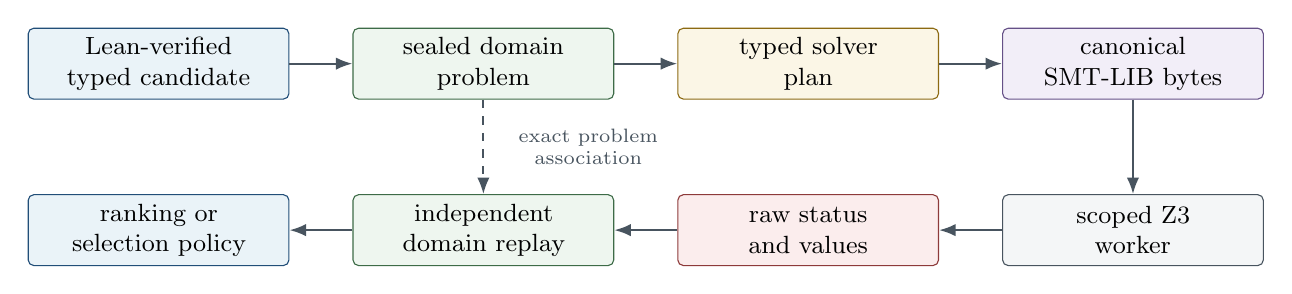
\begin{tikzpicture}[node distance=12mm and 8mm]
  \node[bluebox] (typed) {Lean-verified\\typed candidate};
  \node[greenbox,right=of typed] (sealed) {sealed domain\\problem};
  \node[goldbox,right=of sealed] (plan) {typed solver\\plan};
  \node[purplebox,right=of plan] (bytes) {canonical\\SMT-LIB bytes};
  \node[graybox,below=12mm of bytes] (z3) {scoped Z3\\worker};
  \node[redbox,left=of z3] (raw) {raw status\\and values};
  \node[greenbox,left=of raw] (replay) {independent\\domain replay};
  \node[bluebox,left=of replay] (policy) {ranking or\\selection policy};
  \draw[flow] (typed) -- (sealed);
  \draw[flow] (sealed) -- (plan);
  \draw[flow] (plan) -- (bytes);
  \draw[flow] (bytes) -- (z3);
  \draw[flow] (z3) -- (raw);
  \draw[flow] (raw) -- (replay);
  \draw[flow] (replay) -- (policy);
  \draw[dashflow] (sealed.south) --
    node[note,midway,right=1.5mm,text width=21mm]{exact problem\\association}
    (replay.north);
\end{tikzpicture}
\caption{The solver is one stage in a larger checked pipeline.}
\label{fig:semantic-pipeline}
\end{figure}

\section{Symbolic interpretation versus execution}

A symbolic interpreter does not run the candidate on concrete Lean values. It traverses the exact typed term graph and computes expressions in the domain algebra. For Length:

\begin{itemize}
\item an observed list input becomes a natural variable;
\item \code{nil} has length $0$;
\item \code{cons} adds $1$ to the tail length;
\item a supported exact spine case becomes an \code{ite};
\item a provider occurrence uses its explicit transfer law after occurrence-specific authority checks;
\item an opaque argument may be forwarded but cannot be inspected;
\item unsupported demand is a refusal.
\end{itemize}

The same checked problem also supports concrete replay. Given natural input lengths, the evaluator traverses the candidate graph and computes concrete result lengths. Symbolic and concrete semantics should be two views of one domain definition, tested against each other.

\section{Provider laws are assumptions with provenance}

A type signature rarely reveals behavior. The provider \code{List.reverse} has type \code{List a -> List a}, but length preservation is not derivable from that type alone. A domain may admit a law
\[
  \operatorname{len}(\operatorname{reverse}(xs))=\operatorname{len}(xs).
\]
The law must be explicit and associated with the exact provider declaration and occurrence.

The current Length source distinguishes exactly two trust classes for a provider law (\code{LengthProviderTrust} in Djex's private \code{Internal.Semantic.Length}): a context-free assumed law (\code{AssumedProviderLaw}), and a law on a class-constrained provider that becomes usable only after the occurrence's ground constraints have been discharged independently (\code{AssumedProviderLawConditionalOnConstraintDischarge}). Leant's handoff picks the class purely from the exact inventory scheme: an empty leading context yields the first, a nonempty one the second. A Lean-proved law is proposed, not implemented. The source never infers a transfer from a provider's name, and Z3 is never type-class or dictionary authority.

A result conditional on provider laws should say so. If a provider law is false, both symbolic Z3 reasoning and concrete domain replay can agree with each other while disagreeing with the actual Lean function. A future proof path should link provider laws to Lean theorems whenever possible.

\begin{trustbox}
Independent replay protects against solver and parser mistakes. It does not protect against a wrong domain semantics or false provider assumption shared by both translation and replay. Positive proof artifacts must ultimately connect those assumptions to Lean.
\end{trustbox}

\section{Exactness, over-approximation, and under-approximation}

A domain interpretation may be exact, over-approximate, or under-approximate.

\begin{description}
\item[Exact] Every modeled behavior corresponds to the source abstraction, and every source behavior in scope is represented.
\item[Over-approximation] The model admits all real behaviors and possibly extra behaviors. If no bad modeled behavior exists, no real bad behavior exists; spurious counterexamples are possible and must be replayed.
\item[Under-approximation] The model represents only some real behaviors. Found counterexamples can be real after replay; absence of a counterexample cannot justify pruning or proof.
\end{description}

Sound prefix pruning requires an over-approximation of all completions. Bounded testing and bounded unfolding are under-approximations and may only produce witnesses. These directions are easy to reverse accidentally.

\section{Contract roles}

A contract should not infer semantics from a type constructor's spelling. It supplies a source-ordered role vector, arity-checked against the exact target. (The implemented Length domain admits exactly two target roles, \code{observed-spine} and \code{unobserved-target}, and two provider-argument roles, \code{spine} and \code{unobserved}; richer vocabularies with callbacks or result components are design space, not current code.)

For example, a function may accept two lists but observe only the first, or return a pair of observed lists. The product Length domain has a distinct nominal contract and problem type for two result spines; it is not a cast of scalar evidence.

\section{Closed interpretation policies}

The set of supported cases is itself policy. A candidate that pattern-matches on a list may require exact authority that the matched datatype is the configured spine and that constructor fields are understood. A provider with a nonempty class context may require a restricted resolver and independent ground discharge. A callback may be opaque in one domain and an uninterpreted function in another.

Policy should be represented by closed constructors, not arbitrary callbacks that can smuggle untracked semantics into the interpreter. Changing policy changes the encoding identity.

\section{Failure is part of the semantics}

A refusal to model a candidate is not a counterexample and not evidence that the candidate is wrong. Typical refusals include:

\begin{itemize}
\item no exact typed origin;
\item unsupported target shape or role vector;
\item unresolved or ambiguous spine/provider identity;
\item unsupported term-graph node or demand on an opaque value;
\item provider certificate mismatch;
\item class-resolution authority unavailable;
\item graph, syntax, numeral, or evaluation-step limit exceeded;
\item fingerprint or rendering limit exceeded.
\end{itemize}

Ranking can retain the candidate in a neutral tier. Filtering must preserve it unless the explicit policy says inapplicability is fatal. The current Length filter retains preparation refusals.

\chapter{Typed plans, canonical bytes, and fingerprints}
\label{chap:canonical}

\section{Text must not become the semantic authority}

It is tempting to construct an SMT-LIB string and later treat that string as the meaning of the query. This creates several problems:

\begin{itemize}
\item equivalent formulas may have many textual spellings;
\item escaping and whitespace bugs can alter meaning;
\item string concatenation can bypass sort checks;
\item a renderer bug can make fingerprints identify the wrong plan;
\item later code may parse its own output to rediscover semantics.
\end{itemize}

Djex constructs a typed QF-LIA plan first. Rendering is a bounded projection. The complete fingerprint binds both the structural plan and the resulting command bytes, but replay retains the checked problem rather than reparsing SMT-LIB.

\section{A small typed command language}

The internal AST lives in the private module \code{Language.Haskell.Synthesis.Internal.SMTLib.QFLIA}. Its three types have exactly these constructors (strictness annotations omitted):

\begin{lstlisting}[language=HaskellX,caption={The typed QF-LIA plan, verbatim constructor names from the private Djex module Internal.SMTLib.QFLIA.}]
data QFLIAIntegerExpression
  = QFLIAIntegerSymbol [Word8]
  | QFLIANaturalNumeral Natural
  | QFLIAIntegerSum [QFLIAIntegerExpression]
  | QFLIAIntegerScale Natural QFLIAIntegerExpression
  | QFLIAIntegerDifference QFLIAIntegerExpression QFLIAIntegerExpression
  | QFLIAIntegerBinaryApplication [Word8]
      QFLIAIntegerExpression QFLIAIntegerExpression
  | QFLIAIntegerIf QFLIABooleanExpression
      QFLIAIntegerExpression QFLIAIntegerExpression

data QFLIABooleanExpression
  = QFLIABooleanTruth Bool
  | QFLIAIntegerEqual QFLIAIntegerExpression QFLIAIntegerExpression
  | QFLIAIntegerAtMost QFLIAIntegerExpression QFLIAIntegerExpression
  | QFLIABooleanNot QFLIABooleanExpression
  | QFLIABooleanAll [QFLIABooleanExpression]

data QFLIACommand
  = QFLIASetLogic [Word8]
  | QFLIASetOption [Word8] [Word8]
  | QFLIADefineBinaryInteger [Word8] [Word8] [Word8] QFLIAIntegerExpression
  | QFLIADeclareInteger [Word8]
  | QFLIAAssert QFLIABooleanExpression
  | QFLIACheckSatisfiable
  | QFLIAGetValues [QFLIAIntegerExpression]
\end{lstlisting}

Notice what is absent: there is no disjunction, no strict comparison, no negative literal, and no general multiplication. Strict comparison is written as the negation of an at-most; ``or'' never arises because the Length formula language itself has only truth, equality, at-most, negation, and finite conjunction; and the only subtraction is the one inside the monus helper's body. A constructor cannot accidentally place an integer expression where a Boolean formula is required, and the renderer (\code{renderQFLIACommand}) has one canonical spelling for each node: an empty sum renders as \code{0}, a one-term sum or one-clause conjunction renders as its only member, an empty conjunction renders as \code{true}, and every command ends with exactly one line feed.

\section{Canonicalization choices}

Canonical rendering should specify:

\begin{itemize}
\item declaration order;
\item input-symbol naming from source positions;
\item private-witness naming from deterministic traversal order;
\item helper-definition order;
\item operand order for associative forms;
\item decimal numeral spelling;
\item whitespace and line endings;
\item whether redundant assertions are retained;
\item exact status and value-request sequence.
\end{itemize}

Canonical does not mean mathematically simplest. It means one deterministic representation for one typed plan under one schema.

\section{The current Length preamble}

The scalar and binary-product translators emit an input-only \QFLIA{} program. The fixed preamble:

\begin{enumerate}
\item enables model production;
\item fixes the random seed to $1$;
\item sets logic \QFLIA;
\item defines natural monus as \code{djex_nat_monus};
\item defines binary minimum as \code{djex_nat_min};
\item defines binary maximum as \code{djex_nat_max}.
\end{enumerate}

The query then declares the source input symbols \code{djex_length_input_0}, \code{djex_length_input_1}, \ldots{} in source-position order, declares any private quotient/remainder witness pairs, asserts nonnegativity of every input, asserts the witness constraints, asserts the combined bad-state condition, and calls \code{check-sat} (see \code{sealLengthSMTLibQuery} in the private \code{Internal.Semantic.Length.SMTLib}). A separate optional command, \code{(get-value (djex_length_input_0 ...))}, requests values for all and only the source input symbols; a nullary problem has no such command.

The scalar translator schema is currently tagged \code{djex-length-z3-qf-lia-smtlib2/v2}; the binary-product sibling has a distinct schema. These tags identify translation formats, not the versionless Leant JSON configuration grammar.

\section{Why separate check bytes and value-request bytes}

The check program is valid regardless of status. The value request is sent only after \sat. Keeping the artifacts separate prevents a model request from being blindly issued after \unsat{} or \unknown{} and makes the protocol state explicit.

For a nullary problem there are no input values to request. A satisfiable nullary bad state is replayed without model bindings.

\section{Structural fingerprints}

A fingerprint is a complete, versioned canonical encoding of tagged structural fields---a structural key, not a digest, so equality never depends on accepting a hash collision (SHA-256 appears only inside a fingerprint as the value of an executable-image field). Different subject types prevent accidental comparison of, for example, an inventory fingerprint with a candidate fingerprint.

The Length problem and query bind identities for:

\begin{itemize}
\item semantic domain;
\item exact inventory and spine model;
\item provider-law inventory;
\item interpretation and encoding policy;
\item contract;
\item typed candidate graph;
\item complete behavioral problem;
\item typed query plan and schema;
\item rendered check and value-request bytes.
\end{itemize}

Live execution adds separate identity for the observed executable, protocol, options, and resource limits. This avoids pretending that the same mathematical query run by two different solver envelopes is the same execution artifact.

\section{Fingerprints are association, not proof}

A fingerprint can establish that an artifact belongs to the exact problem that produced it. It cannot establish that the problem encoding is sound, that a provider law is true, or that an \unsat{} response is trustworthy. This is why Djex's generic module says ``association is not certification.''

\section{Versioning strategy}

Every semantic change that can alter meaning or accepted artifacts must change a schema identity. Examples include:

\begin{itemize}
\item different input-symbol order;
\item a changed monus definition;
\item added or removed nonnegativity assumptions;
\item new provider-law interpretation;
\item a different sequence representation;
\item changed fixedpoint rule generation;
\item different objective priority;
\item changed incremental scope protocol.
\end{itemize}

Leant's current configuration files are deliberately versionless and experimental: superseded shapes live in Git history. That source-file policy is compatible with versioned internal semantic fingerprints. One governs user-facing decoder compatibility; the other prevents evidence reassociation.

\section{Bounds before fingerprints}

Fingerprint builders themselves consume resources. Djex bounds command bytes, fingerprint bytes, symbol bytes, syntax nodes, numeral bits, collection widths, and retained artifact payloads. A value too large to fingerprint safely is rejected before it enters an opaque checked object.

The default Length query limits in the inspected Djex tree admit $65{,}536$ bytes per command artifact, $262{,}144$ fingerprint-builder bytes, and $4{,}096$ bits per rendered natural numeral. These defaults are policy, not mathematical constants.

\begin{sourcebox}
See \dpath{synthesis/internal/Language/Haskell/Synthesis/Internal/Semantic/Length/SMTLib.hs} and \dpath{synthesis/internal/Language/Haskell/Synthesis/Internal/SMTLib/QFLIA.hs}.
\end{sourcebox}

\chapter{Owning the Z3 process}
\label{chap:process}

\section{The process lifecycle is a state machine}

A live solver integration is not merely \code{write}; \code{read}. It owns a sequence:

\begin{enumerate}
\item admit and validate pure execution policy;
\item resolve and inspect the executable;
\item create a fresh isolated workspace;
\item spawn with exact arguments and environment;
\item perform readiness/capability probes;
\item lend a scoped ready worker;
\item execute bounded serialized transactions;
\item close stdin or request exit;
\item wait, terminate, and escalate if necessary;
\item release descriptors and workspace;
\item report whether cleanup was incomplete.
\end{enumerate}

Every transition can fail. Failures during cleanup must not overwrite a more important callback exception, but incomplete cleanup should remain observable.

\section{No shell and no ambient environment}

The current execution profile uses a fixed direct argument prefix, policy-derived resource arguments, and an exact empty child environment. It does not invoke a shell or inherit ambient variables. A fresh empty working directory is selected instead of inheriting the caller's directory.

These choices reduce accidental dependence on locale, configuration files, path search, user startup scripts, and environment secrets. They also make the execution identity easier to describe.

\section{Executable admission and digest pinning}

A configuration can contain an expected SHA-256 digest. Activation policy separately decides whether an unpinned executable is allowed. This separation is important: successfully decoding a path and digest field does not grant permission to execute it.

The live opener must defend resolution, hashing, and spawn against path replacement races. Djex exposes four launch strategies (\code{LengthSMTLibExecutableLaunchStrategy}): a portable path-snapshot-then-spawn strategy, and three Linux descriptor-bound strategies that open the executable once, copy its bytes into a sealed anonymous memory image, compare the digest, and spawn from that descriptor, optionally after effective-ID or \code{AT_EXECVE_CHECK} access checks on the source and the staged image. The three descriptor-bound launches share one pipeline (\code{openDescriptorBoundProcessWith}, parameterized by a \code{DescriptorBoundLaunchPolicy} record, in the private \code{Internal.SMTLib.Z3.Process}) and one narrow C helper, \dpath{synthesis/cbits/z3_descriptor_spawn.c}, compiled only on Linux; elsewhere they fail closed before any spawn.

The public API reveals only closed classifications such as whether a digest expectation exists and which launch strategy was selected. It does not leak path or digest bytes through ordinary errors.

\section{Capability probing}

A process that launches successfully is not yet a ready Length solver. The readiness probe (private \code{Session/Capability.hs}) is a fixed four-write handshake; each write ends with a fresh positional \code{echo} barrier whose exact quoted string must come back before the next phase may begin:

\begin{enumerate}
\item the startup option \code{(set-option :print-success false)}: nothing but the barrier echo may come back;
\item a reset, the canonical Length preamble, one declared integer asserted equal to $0$, and \code{(check-sat)}: the solver must answer \sat;
\item \code{(get-value ...)} for that constant: the solver must answer exactly \code{((djex_capability_input 0))};
\item a reset, the preamble, the constant asserted equal to both $0$ and $1$, and \code{(check-sat)}: the solver must answer \unsat.
\end{enumerate}

Together these demonstrate acceptance of the startup options, \QFLIA{} status framing in both directions, value retrieval in the exact shape the decoder expects, reset behavior, whitespace and framing rules across write boundaries, and transport liveness. The probe establishes only this demonstrated profile. It does not certify arbitrary Z3 capabilities, resource-limit behavior, or semantic soundness.

\section{Causal framing}

A pipe is a byte stream, not a request/response message channel. Output may be chunked arbitrarily. Diagnostics can be delayed. A read can return half an S-expression or several responses at once.

Djex's internal causal driver uses barriers/markers and a bounded stream parser to associate complete responses with transaction order. Public callers cannot inspect or retain the process handle, transcript, barrier, ordinal, or decoded valuation. This prevents a later API layer from accidentally bypassing the transaction owner.

\section{One query transaction}

A scalar transaction conceptually proceeds as follows:

\begin{enumerate}
\item reset the solver to the probed clean state;
\item submit the sealed check bytes and a causal marker;
\item parse exactly one status response;
\item if \sat{} and inputs exist, submit the sealed value-request bytes and another marker;
\item parse exactly the expected input bindings;
\item validate and replay the assignment;
\item associate the observation with exact query and execution identities;
\item make the session ready for the next reset or close it on protocol failure.
\end{enumerate}

A malformed model, stale output, unexpected success token, extra payload, or replay failure is a transaction failure. The driver does not reinterpret it as \unknown{} or as a harmless non-counterexample.

\section{Budgets and deadlines}

Solver-side timeout/resource options and host-side deadlines solve different problems. A cooperative solver timeout may not fire if the process is stuck outside the relevant check. A host deadline can interrupt transport and initiate cleanup, but cannot prove the child honored internal resource limits.

The execution policy binds finite values for solver timeout, solver resource limit, host deadline, response limits, and optional shared usable-work budget. The host deadline must exceed the solver timeout by a minimum margin (currently $100$ ms, \code{z3SMTLibMinimumHostDeadlineMarginMilliseconds}) so there is time to receive and parse a cooperative response. The solver timeout and resource limit are passed on the command line as \code{timeout=} and \code{rlimit=} arguments, and both must be finite and nonzero.

A shared usable-work deadline can cover session opening and several queries. The newer scoped token checks owner thread and dynamic extent at runtime; rank-$N$ polymorphism alone cannot prevent a closure or forked thread from retaining a phantom token.

\section{Query leases and maximum transactions}

A live scope admits a bounded number of scalar-plus-product transactions in total; the current public default is $64$. The bound limits state growth and prevents an accidentally retained worker from becoming a general unbounded solver service.

A lease is spent even when a transaction fails after admission. Rolling back real solver work would make budgets dishonest and can enable retry amplification.

\section{Cancellation and cleanup}

Cancellation has at least three layers:

\begin{itemize}
\item stop admitting new transactions;
\item interrupt or terminate the child process;
\item reclaim pipes, descriptors, threads, and workspace.
\end{itemize}

Asynchronous exceptions complicate ownership. The scoped API begins durable cleanup before propagating callback exceptions across the boundary. Public errors expose a sanitized primary class and whether cleanup was incomplete, not child-controlled output or sensitive paths.

\begin{pitfall}
Killing a process is not the same as completing cancellation. If reader threads, descendants, descriptors, or temporary directories remain, later runs can observe interference or leak resources.
\end{pitfall}

\section{Concurrency}

One ready worker serializes its protocol. Parallel candidate checks should use independent workers or a higher-level scheduler, not interleave commands on one stdin stream. Z3 contexts in language bindings also have thread-affinity/thread-safety constraints; a subprocess does not eliminate the need for ownership discipline.

The planned sketch solver may benefit from long-lived incremental sessions, but parallelism should occur across independently scoped sessions or solver clones with explicit identities.

\begin{sourcebox}
See \dpath{synthesis/src/Language/Haskell/Synthesis/Semantic/Length/SMTLib/Execution.hs}, \dpath{synthesis/src/Language/Haskell/Synthesis/Semantic/Length/SMTLib/Live.hs}, and the private \dpath{synthesis/internal/Language/Haskell/Synthesis/Internal/SMTLib/Z3/Process.hs} and \dpath{synthesis/internal/Language/Haskell/Synthesis/Internal/Semantic/Length/SMTLib/Session/} modules.
\end{sourcebox}

\chapter{From observations to evidence}
\label{chap:evidence}

\section{A useful evidence ladder}

Results can be arranged by what they authorize, not by how impressive they sound:

\begin{longtable}{@{}L{0.22\textwidth}L{0.25\textwidth}L{0.47\textwidth}@{}}
\toprule
Artifact & What it supports & What it does not support \\
\midrule
\endhead
Raw \sat{} + values & Candidate input for decoding & Rejection before association and replay \\
Associated solver observation & Exact provenance of the run & Behavioral correctness or violation by itself \\
Replayed counterexample & Rejection of that exact candidate under the domain model & Positive correctness of another candidate \\
Finite-box positive receipt & Property on an explicitly enumerated finite box & Universal correctness outside the box \\
Complete applicable-domain receipt & Property over an exactly traversed finite applicable domain & Claims beyond the domain/model/provider assumptions \\
Raw \unsat{} & Useful heuristic that the encoded bad state has no model & Automatic proof authority in current Djex \\
Lean-checked theorem & Positive claim expressed and checked in Lean & Any stronger claim than the theorem states \\
\bottomrule
\end{longtable}

\section{Why counterexamples are easy to trust}

A universal property is refuted by one witness. The host can evaluate that witness directly. Even if Z3 reached it through complex heuristics, the final check is small:
\[
  P(x)=\text{true},\qquad Q(x,C(x))=\text{false}.
\]

This asymmetry lets an untrusted or merely heuristic solver be operationally useful. The solver is a witness generator; the domain evaluator is the authority.

\section{Why positive results are harder}

A universal positive claim requires excluding every counterexample. There are three main ways to earn that authority:

\begin{enumerate}
\item \term{Finite exhaustion}: the domain is finite and every applicable assignment is replayed.
\item \term{Trusted exact decision procedure}: the application explicitly places the exact solver/encoding in its trusted base.
\item \term{Proof production}: generate a theorem or certificate checked by a trusted proof checker such as Lean.
\end{enumerate}

The current architecture uses the first where bounded or complete finite domains are available and plans the third for proof-grade results. It deliberately does not silently choose the second.

\section{Behavioral statuses}

Djex's solver-neutral vocabulary distinguishes:

\begin{description}
\item[Behavior established] A domain-owned verifier has established the property under its declared scope.
\item[Behavior violated] A domain-owned counterexample has been reproduced.
\item[Behavior validated within] A bounded region has been exhaustively checked.
\item[Behavior unknown] No supported conclusion was reached.
\end{description}

These are report categories. Public construction of a raw observation is harmless because it carries no candidate and no authority. Opaque evidence requires private domain constructors and exact replay.

\section{Fail closed in semantics, preserve in policy}

Two superficially opposite rules coexist:

\begin{itemize}
\item The semantic adapter \term{fails closed}: it refuses to invent meaning for unsupported input.
\item Conservative ranking/filtering \term{preserves candidates}: a refusal or operational failure does not masquerade as a counterexample.
\end{itemize}

Failing closed means ``do not claim to understand.'' Preserving means ``do not punish the candidate for our lack of understanding.'' An explicitly strict user policy may decide otherwise, but the distinction must remain visible.

\section{Selection needs stronger association than ranking}

A ranking is a permutation. A sealing layer can verify that every input occurrence appears exactly once and in the chosen order. Hard filtering is a partition: each verified occurrence must appear exactly once in either retained or rejected output, and every rejection must carry domain-authorized evidence.

The generic \code{BehavioralSelection} boundary in Leant checks occurrence membership, totality, and original-order association. It does not establish behavior itself. Length-specific private builders decide that only an independently replayed counterexample authorizes rejection.

\section{Batch failures preserve the original batch}

If a selection operation encounters an operational or sealing failure, the current Length path preserves the complete original callback batch. This prevents partial solver progress from causing nondeterministic omission.

Candidate-local outcomes remain visible: a preparation refusal, unknown solver status, positive bounded receipt, or unassessed candidate is retained with an explicit retention class.

\section{Conditional claims}

A receipt may be conditional on:

\begin{itemize}
\item the configured finite-spine model;
\item provider laws and their ground discharges;
\item an exact interpretation policy;
\item finite input bounds;
\item an over-approximation profile;
\item a specific solver envelope if external trust is selected.
\end{itemize}

The user-facing presentation should carry these conditions instead of printing a context-free word such as ``verified.''

\begin{checkpoint}
Ask of every result: What exact action may this artifact authorize? Ranking? Rejection? A bounded badge? A theorem? If the answer is unclear, the type or presentation is too weak.
\end{checkpoint}

\chapter{Incrementality, determinism, and CEGIS-ready state}
\label{chap:incrementality}

\section{Two kinds of reuse}

A synthesis system can reuse work at two distinct levels:

\begin{description}
\item[Semantic reuse] Store concrete counterexample inputs and replay them against new candidates without a solver.
\item[Solver-state reuse] Keep declarations, sample constraints, learned clauses, and scopes inside a live incremental Z3 session.
\end{description}

Semantic reuse is simpler and already present in the Length counterexample bank. Solver-state reuse is more powerful for typed sketches but needs a new protocol.

\section{Counterexample-guided inductive synthesis}

A canonical CEGIS loop is:

\begin{enumerate}
\item choose a candidate satisfying all known samples;
\item ask whether the candidate has any counterexample;
\item if a replayed counterexample is found, add it to the sample bank;
\item repeat;
\item stop with a positive proof/claim, an exhausted finite grammar, or an explicit budget result.
\end{enumerate}

There are two solvers conceptually:

\begin{itemize}
\item the \term{synthesis solver} chooses candidate selectors consistent with samples;
\item the \term{verification solver} searches for a fresh input violating the chosen candidate.
\end{itemize}

They may both be Z3 sessions, but they have different variables, assertions, artifacts, and trust directions. The verification model proposes a counterexample; the synthesis model proposes a program completion.

\begin{figure}[htbp]
\centering
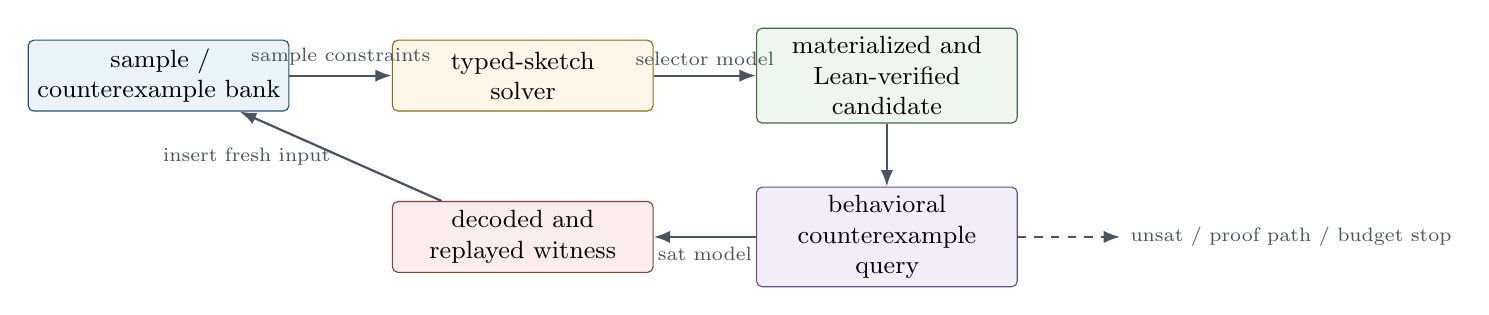
\begin{tikzpicture}[node distance=8mm and 13mm]
  \node[bluebox] (samples) {sample /\\counterexample bank};
  \node[goldbox,right=of samples] (synth) {typed-sketch\\solver};
  \node[greenbox,right=of synth] (candidate) {materialized and\\Lean-verified candidate};
  \node[purplebox,below=of candidate] (verify) {behavioral\\counterexample query};
  \node[redbox,left=of verify] (cex) {decoded and\\replayed witness};
  \draw[flow] (samples) -- node[note,above]{sample constraints} (synth);
  \draw[flow] (synth) -- node[note,above]{selector model} (candidate);
  \draw[flow] (candidate) -- (verify);
  \draw[flow] (verify) -- node[note,below]{sat model} (cex);
  \draw[flow] (cex) -- node[note,left]{insert fresh input} (samples);
  \draw[dashflow] (verify.east) -- ++(13mm,0) node[note,right]{unsat / proof path / budget stop};
\end{tikzpicture}
\caption{The planned CEGIS feedback loop.}
\label{fig:cegis}
\end{figure}

\section{Monotone sample growth}

If the grammar and semantics are fixed, adding counterexamples only strengthens synthesis constraints. Learned nogoods derived from unsatisfiable selector assumptions remain valid while the sample bank grows, but not after changing:

\begin{itemize}
\item provider inventory;
\item grammar productions or costs;
\item semantic domain or encoding profile;
\item type target or role vector;
\item candidate-size bound;
\item sample representation.
\end{itemize}

Nogoods and sample banks must therefore be scoped by exact fingerprints.

\section{Semantic signatures}

Before full solver-selected sketches, a smaller step is available in principle (it is not in the current tree): evaluate enumerated candidates on the current sample bank and compute a semantic signature:
\[
  \sigma(C)=\bigl(C(x_1),\ldots,C(x_k)\bigr)
\]
under the chosen observation domain. Candidates with the same signature are indistinguishable on known samples.

The search can keep one representative per signature, postpone duplicate classes, or prioritize classes not yet explored. A new counterexample refines the partition. This is a low-risk bridge from post-verification filtering to CEGIS-aware enumeration.

\section{Determinism}

Reproducibility requires more than a fixed random seed. It includes:

\begin{itemize}
\item stable provider and production order;
\item canonical symbol allocation;
\item stable sample order and bank replacement policy;
\item deterministic objective priority;
\item fixed timeout/resource configuration;
\item pinned or observed solver build;
\item stable response normalization;
\item deterministic counterexample simplification;
\item stable tie-breaking after ranking.
\end{itemize}

A solver can still choose a different model after an implementation upgrade. Independent replay protects correctness; reproducibility tests detect presentation and search-order drift.

\section{Incremental state fingerprints}

A future incremental session should bind:

\begin{itemize}
\item base declarations and grammar fingerprint;
\item every asserted sample in order;
\item push/pop or assumption discipline;
\item active selector assumptions;
\item core-production settings;
\item objective order and optimization mode;
\item solver parameters and observed capabilities;
\item transaction ordinal and reset generation.
\end{itemize}

It should expose a typed state transition API rather than generic ``send SMT-LIB'' access.

\section{Recovery}

Once an incremental protocol becomes desynchronized, continuing may produce plausible but stale answers. Conservative recovery is to discard the worker and rebuild from the canonical base plus retained sample bank. Rebuilding is slower but restores a known state.

The sample bank belongs outside the process and survives worker replacement. Learned clauses retained only inside Z3 are an optimization, not semantic authority.


% =============================================================================
\part{Z3 in the Current Leant/Djex System}

\chapter{The four-layer architecture}
\label{chap:current-architecture}

\section{One pipeline, four different kinds of authority}

The current system is easiest to understand as four cooperating components with deliberately noninterchangeable responsibilities:

\begin{description}
\item[Djex search.] Construct type-correct candidate graphs inside a checked synthesis inventory. Djinn searches a logical fragment; Exference searches a richer provider-oriented structural fragment. Djex owns the private names, schemes, term graphs, occurrence certificates, and completeness information needed to explain how a candidate was built.

\item[Lean verification.] Re-elaborate a rendered candidate against the exact requested Lean type in the active project environment. This decides whether the spelling has the intended Lean meaning, resolves implicit arguments and type classes, checks universes and elaboration constraints, and ultimately relies on Lean's kernel for type correctness.

\item[Djex semantic interpretation.] Starting from the exact typed origin of a Lean-accepted candidate, seal a domain-specific behavioral problem. For the implemented Length domain, this means interpreting the candidate as a symbolic transformation of finite spine lengths under an explicit contract and explicit provider laws.

\item[Z3 search.] Determine whether the sealed counterexample condition has a satisfying assignment in the selected SMT theory. In the current domain, the theory is quantifier-free linear integer arithmetic. A returned assignment is decoded and independently replayed by Djex before it can become counterexample evidence.
\end{description}

These responsibilities form a chain, but no component silently inherits the authority of the next one.

\begin{figure}[htbp]
\centering
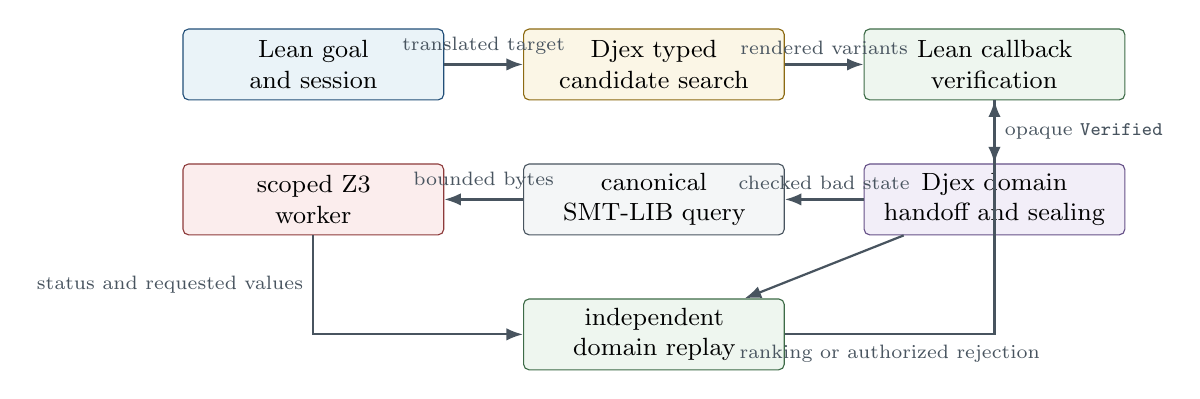
\begin{tikzpicture}[node distance=8mm and 10mm]
  \node[bluebox] (goal) {Lean goal\\and session};
  \node[goldbox,right=of goal] (search) {Djex typed\\candidate search};
  \node[greenbox,right=of search] (lean) {Lean callback\\verification};
  \node[purplebox,below=of lean] (seal) {Djex domain\\handoff and sealing};
  \node[graybox,left=of seal] (query) {canonical\\SMT-LIB query};
  \node[redbox,left=of query] (z3) {scoped Z3\\worker};
  \node[greenbox,below=of query] (replay) {independent\\domain replay};
  \draw[flow] (goal) -- node[note,above]{translated target} (search);
  \draw[flow] (search) -- node[note,above]{rendered variants} (lean);
  \draw[flow] (lean) -- node[note,right]{opaque \code{Verified}} (seal);
  \draw[flow] (seal) -- node[note,above]{checked bad state} (query);
  \draw[flow] (query) -- node[note,above]{bounded bytes} (z3);
  \draw[flow] (z3) |- node[note,left,pos=0.25]{status and requested values} (replay);
  \draw[flow] (seal) -- (replay);
  \draw[flow] (replay) -| node[note,below,pos=0.25]{ranking or authorized rejection} (lean.south);
\end{tikzpicture}
\caption{Current Leant/Djex behavioral-assessment pipeline. The return arrow does not alter Lean's verification receipt; it associates a separate behavioral assessment with that exact occurrence.}
\label{fig:current-pipeline}
\end{figure}

\begin{mentalmodel}
Lean answers ``does this term have the requested type?'' Djex answers ``what checked candidate did that spelling come from, and what does it mean in this observation domain?'' Z3 answers ``is there a mathematical assignment satisfying the encoded bad state?'' Independent replay answers ``does that assignment really violate this exact sealed problem?''
\end{mentalmodel}

\section{Why type correctness is not behavioral correctness}

A type can admit many inhabitants with very different behavior. For example,
\[
  \operatorname{List}\alpha \to \operatorname{List}\alpha
\]
contains, among many others:

\begin{lstlisting}[language=LeanX,caption={Four well-typed inhabitants with different behavior.}]
fun xs => xs
fun xs => xs.reverse
fun _  => []
fun xs => xs ++ xs
\end{lstlisting}

Lean correctly accepts all four at the same type. A type-directed synthesizer may therefore return all four unless additional intent is supplied. A length-preservation contract distinguishes the last two from the first two, but it still does not distinguish identity from reverse. A pointwise sequence contract could distinguish those. This is the central motivation for behavioral synthesis: a type determines the admissible interface; a contract describes some intended semantics within that interface.

The current implementation deliberately applies behavioral reasoning \emph{after} Lean callback verification. Thus Z3 never repairs a type error and never makes an unelaborated candidate acceptable. It only assesses candidates that already crossed the exact Lean boundary.

\section{Candidate groups, variants, and callback verification}

A single semantic candidate graph can have several possible Lean spellings. Implicit arguments, qualification, coercions, constructor syntax, generated lets, and renderer alternatives may cause one spelling to elaborate while another does not. Leant therefore works with candidate groups and verification variants rather than assuming that one pretty-printer output is authoritative.

The callback tries variants in a controlled order. The first accepted variant produces an opaque \code{Verified DetailedVerificationVariant} receipt. A caller can inspect presentation information, but it cannot manufacture a receipt merely by holding the same text.

\begin{trustbox}
A \code{Verified} receipt records callback acceptance of one occurrence. It is not a behavioral certificate, a proof that a provider law is true, or a solver result. Conversely, a behavioral counterexample does not invalidate Lean's type-checking judgment. It says that a well-typed term violates an additional contract.
\end{trustbox}

\section{The exact typed origin}

Behavioral interpretation must not reverse-engineer a term graph from rendered Lean text. The same text can elaborate differently in different environments, and pretty-printing can erase distinctions that matter to the synthesis engine. For typed Exference routes, Leant therefore retains an opaque \code{ExactTypedVariantOrigin} sidecar. It ties the accepted spelling to such facts as:

\begin{itemize}
\item the exact typed candidate graph;
\item the checked synthesis inventory;
\item source and search goals;
\item provider bindings and nominal family identities;
\item renderer ordinal and rendering route;
\item premise layout and request context;
\item the semantic-family provenance discovered during translation.
\end{itemize}

The Length handoff obtains that origin from the \code{Verified} receipt and rerenders it internally. The caller does not separately submit a graph and claim that it corresponds to the accepted text.

\begin{projectnote}
This is why the behavioral layer is currently available only for candidate routes carrying sufficient typed provenance. A text-only candidate may be perfectly good Lean, but the Length interpreter refuses to guess which Djex graph or provider occurrences produced it. In practice this means selecting the Exference engine: Leant's default \code{synth-engine} is \code{djinn}, which supplies no typed graph, so under the default engine every candidate is retained with the payload-free refusal code \code{unsupported-route} and no worker is opened. Use \code{:set synth-engine exference} (or \code{both}) to produce assessable candidates; Leant prints a reminder to that effect when a configuration is activated at startup.
\end{projectnote}

\section{What each repository contributes}

At the inspected snapshots, the source ownership is roughly as follows.

\begin{longtable}{@{}L{0.20\textwidth}L{0.31\textwidth}L{0.43\textwidth}@{}}
\toprule
Layer & Primary repository area & Responsibility \\
\midrule
\endfirsthead
\toprule
Layer & Primary repository area & Responsibility \\
\midrule
\endhead
\bottomrule
\endfoot
Leant REPL and orchestration & \lpath{src/Main.hs}, \lpath{src/Leant/Options.hs} & Session state, commands, candidate scheduling, callback verification, optional Length configuration, result presentation. \\
Leant synthesis bridge & \lpath{src/Leant/Synth/Engine.hs}, \lpath{src/Leant/Synth/Verification.hs} & Candidate groups, exact typed sidecars, rendering, opaque verification receipts. \\
Leant Length adapter & \lpath{src/Leant/Synth/Length/} & Passive Lean-named contracts, exact handoff, startup/request policy, post-verification ranking, hard selection, counterexample-bank ownership, diagnostics. \\
Djex checked synthesis foundation & \dpath{synthesis/src/Language/Haskell/Synthesis/} and private counterparts & Inventories, names, schemes, typed candidates, occurrence certificates, fingerprints, search products. \\
Djex Length semantics & \dpath{synthesis/src/Language/Haskell/Synthesis/Semantic/Length.hs} and \dpath{synthesis/src/Language/Haskell/Synthesis/Semantic/Length/} & Checked finite-spine contracts, symbolic interpretation, concrete evaluation, counterexample evidence, canonical queries. \\
Djex solver boundary & \dpath{synthesis/src/Language/Haskell/Synthesis/Semantic/Length/SMTLib/} and private \filepath{Internal/SMTLib} modules & QF-LIA rendering, bounded parsing, protocol framing, live Z3 process ownership, replay association. \\
Z3 & \zpath{src/} plus the public executable/API & SMT solving, model construction, fixedpoint reasoning, optimization and other solver capabilities. \\
Lean project backend & External Lean project/toolchain driven by Leant & Elaboration, name resolution, type-class synthesis, generated declaration checking, kernel authority. \\
\end{longtable}

\begin{sourcebox}
For the broad architecture, compare the existing \lpath{docs/Leant_Overview/Leant_Overview.tex}, \lpath{docs/Djex_Leant_Codebase_Walkthrough/Djex_Leant_Codebase_Walkthrough.tex}, and \lpath{docs/Z3_Behavioral_Synthesis_Proposal/Z3_Behavioral_Synthesis_Proposal.tex}. The current narrow behavioral entrances are concentrated in \lpath{src/Leant/Synth/Length/Handoff.hs}, \lpath{src/Leant/Synth/Length/Integration.hs}, \lpath{src/Leant/Synth/Length/Ranking.hs}, and \lpath{src/Leant/Synth/Length/Selection.hs}.
\end{sourcebox}

\chapter{The implemented finite-spine Length domain}
\label{chap:length-domain}

\section{Why start with length?}

List length is a useful first behavioral observation because it is simple enough for exact arithmetic reasoning yet discriminating enough to improve synthesis. It has several engineering advantages:

\begin{itemize}
\item element values can remain completely opaque;
\item finite lists are summarized by natural numbers;
\item constructors have simple transfers: zero contributes $0$ and a step contributes $n+1$;
\item many library functions have affine or piecewise-linear length behavior;
\item contract violation becomes a quantifier-free linear-integer formula;
\item counterexamples are small vectors of natural numbers that are easy to replay and display.
\end{itemize}

It also exposes the hard parts that future domains share: exact datatype identity, provider-law assumptions, symbolic case analysis, typed candidate provenance, canonical translation, model replay, evidence association, and process isolation.

\section{A spine rather than a built-in-name convention}

The semantic object is a unary finite recursive \emph{spine}, not necessarily Lean's built-in \code{List}. A contract names:

\begin{itemize}
\item the family;
\item its zero constructor;
\item its step constructor;
\item the structurally recursive field of the step constructor, validated by Djex;
\item the roles of the target's source-ordered arguments.
\end{itemize}

For ordinary lists, the intended pattern is morally
\[
  \operatorname{nil}:F\alpha,
  \qquad
  \operatorname{cons}:\alpha\to F\alpha\to F\alpha.
\]
The Length model observes only how many step constructors occur. Payload fields are opaque and cannot be inspected merely because the solver would find it convenient.

\begin{pitfall}
The spelling \code{List} does not grant list semantics. The contract's Lean names are matched against the exact nominal family and constructor provenance retained from translation. A different declaration with a similar shape or name is not silently coerced into the model.
\end{pitfall}

\section{Scalar and binary-product domains}

The current code has two nominally distinct domains.

\begin{description}
\item[Scalar finite-spine length.] The modeled result is one finite spine. A contract can relate its length to the modeled input lengths.

\item[Binary-product finite-spine lengths.] The normalized result root must be canonical Lean \code{Prod}, and both source-ordered fields must be the configured spine family. The contract may relate both output lengths to the inputs, for example
\[
  r_0+r_1=n.
\]
This supports early reasoning about functions such as partitioning or splitting even though element membership and order are not yet modeled.
\end{description}

The two domains reuse arithmetic machinery but retain different problem, query, evidence, bank, protocol, and fingerprint types. Identical rendered SMT-LIB bytes do not make scalar evidence valid for the product domain.

\section{The passive contract}

A Leant Length contract is a passive source value. It contains no process handle and grants no permission to run Z3. Its major fields are:

\begin{longtable}{@{}L{0.25\textwidth}L{0.69\textwidth}@{}}
\toprule
Field & Meaning \\
\midrule
\endfirsthead
\toprule
Field & Meaning \\
\midrule
\endhead
\bottomrule
\endfoot
Spine identity & Exact Lean family, zero-constructor, and step-constructor names. \\
Target argument roles & A source-ordered vector with one entry per physical target argument, each either \code{observed-spine} (a modeled spine of the configured family; observed positions are numbered compactly from zero) or \code{unobserved-target} (an opaque token that may be forwarded but never inspected, called, or destructured). Roles are not guessed from types. \\
Candidate case policy & Either reject candidate case analysis or admit the exact finite-spine zero/step case semantics supported by the current interpreter. \\
Precondition & A solver-neutral Length formula describing when the contract applies. \\
Postcondition & A solver-neutral Length formula relating modeled inputs and result length or result pair. \\
Provider laws & Explicit assumptions for exact provider names, each with argument roles and a transfer expression. \\
\end{longtable}

A scalar contract with one modeled input can express length preservation as
\[
  P(n)=\top,
  \qquad
  Q(n,r)\equiv r=n.
\]
A nonempty-only contract can use
\[
  P(n)\equiv n>0.
\]
A binary-product split contract might say
\[
  P(n)=\top,
  \qquad
  Q(n,r_0,r_1)\equiv r_0+r_1=n.
\]

\begin{trustbox}
A contract is an assertion of intended semantics, not evidence that the named declarations really have those semantics. Exact names and schemes are checked at handoff. Provider transfer laws remain explicit assumptions unless separately connected to Lean proofs.
\end{trustbox}

\section{Provider laws}

A synthesized candidate often calls an existing function whose source is not symbolically expanded. To reason about such a call, the domain needs a transfer law. For example:

\begin{align*}
  \operatorname{len}(\operatorname{reverse}(xs)) &= \operatorname{len}(xs),\\
  \operatorname{len}(\operatorname{append}(xs,ys)) &=
    \operatorname{len}(xs)+\operatorname{len}(ys),\\
  \operatorname{len}(\operatorname{drop}(k,xs)) &=
    \operatorname{len}(xs)\mathbin{\dot{-}}k.
\end{align*}

Leant does not infer these laws from names, documentation, source text, or testing. A law identifies an exact provider occurrence through the checked inventory and supplies source-ordered argument roles plus a transfer expression. Djex verifies that the provider's scheme and occurrence certificate are compatible with use of the law.

Some providers have class constraints. The current associated-provider path may use one restricted closed scheme only after its ground obligations are discharged against the exact inventory and occurrence-specific certificate chain. Z3 is never asked to decide whether a Lean type-class instance exists.

\begin{projectnote}
This separation is crucial. Arithmetic reasoning may depend on the assumption that an exact provider preserves length; dictionary resolution and occurrence identity remain Djex/Lean facts. ``Z3 found a model'' cannot authorize a type-class dictionary or retroactively validate a provider binding.
\end{projectnote}

\section{Symbolic values in the Length interpreter}

For a target with modeled input lengths $n_0,\ldots,n_{k-1}$, the interpreter evaluates the exact typed candidate graph to a symbolic result expression. Relevant nodes include:

\begin{itemize}
\item locals and lambda-bound variables;
\item applications and explicit type applications;
\item lets and supported tuple forms;
\item zero and step constructors of the configured spine;
\item exact spine case analysis under the selected case policy;
\item calls to providers with admitted occurrence-specific laws;
\item opaque tokens that may be transported but not inspected.
\end{itemize}

A zero constructor denotes $0$. A step constructor whose recursive field has length $e$ denotes $e+1$. A supported exact case on a spine of symbolic length $n$ has the essential form
\[
  \operatorname{caseLen}(n,z,s)
  =\operatorname{ite}\bigl(n=0,\ z,\ s(n\mathbin{\dot{-}}1)\bigr),
\]
where
\[
  a\mathbin{\dot{-}}b=\max(a-b,0)
\]
is natural monus. Both branches are interpreted. The set of provider-law assumptions used by the candidate is conservatively retained even if arithmetic simplification later removes a branch.

Unsupported demand is a refusal. For example, if the candidate attempts to inspect an opaque element payload, call an unmodeled callback, open an unsupported recursive structure, or use an unrecognized provider occurrence, the interpreter does not invent an unconstrained arithmetic result and call it sound.

\section{Sealing order}

The checked values form a one-way chain:

\begin{enumerate}
\item seal an exact synthesis inventory and spine model;
\item seal an interpretation policy;
\item seal a Length session associating inventory, spine, provider-law table, and policy;
\item revalidate the passive contract inside that session;
\item seal the exact typed candidate against that contract;
\item derive the substituted counterexample condition;
\item seal a canonical query and its complete structural fingerprint.
\end{enumerate}

Each opaque value is constructible only after the checks for that stage succeed. A downstream caller cannot take a checked candidate from one inventory, a contract from another session, and bytes from a third query and associate them by record construction.

\begin{figure}[htbp]
\centering
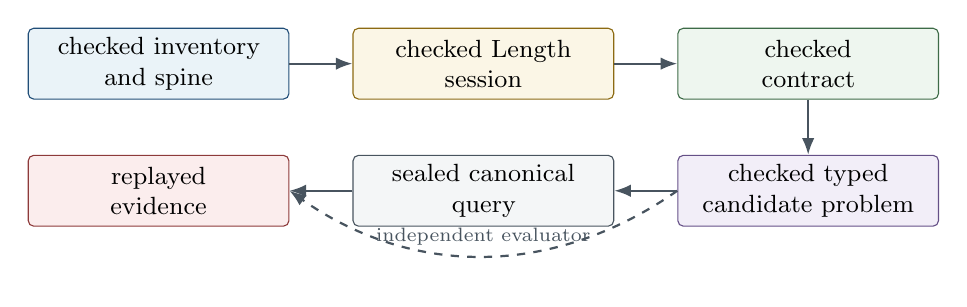
\begin{tikzpicture}[node distance=7mm and 8mm]
  \node[bluebox] (inv) {checked inventory\\and spine};
  \node[goldbox,right=of inv] (session) {checked Length\\session};
  \node[greenbox,right=of session] (contract) {checked\\contract};
  \node[purplebox,below=of contract] (candidate) {checked typed\\candidate problem};
  \node[graybox,left=of candidate] (query) {sealed canonical\\query};
  \node[redbox,left=of query] (evidence) {replayed\\evidence};
  \draw[flow] (inv) -- (session);
  \draw[flow] (session) -- (contract);
  \draw[flow] (contract) -- (candidate);
  \draw[flow] (candidate) -- (query);
  \draw[flow] (query) -- (evidence);
  \draw[dashflow] (candidate.west) to[bend left=35] node[note,above]{independent evaluator} (evidence.east);
\end{tikzpicture}
\caption{The current Length authority chain. Every arrow is a validating constructor or replay gate, not a cast.}
\label{fig:length-sealing}
\end{figure}

\section{The Leant handoff in detail}

The public scalar entrance \code{prepareCheckedLengthProblem} takes a passive \code{LeanLengthContract} and an opaque callback-accepted receipt. Its fail-closed sequence is approximately:

\begin{enumerate}
\item require the typed candidate route and exact semantic sidecar;
\item require the source, fit, engine, and search fragments to retain the expected correspondence;
\item reject caller or constructor premises outside the current modeled entrance;
\item require the request context and goal to match the translated source goal;
\item rerender the opaque exact origin, require a unique expected rendering, and require the accepted text and renderer ordinal to match;
\item resolve the configured spine family and constructors against retained semantic-family provenance;
\item resolve every provider law against exact provider bindings, rejecting missing or ambiguous names;
\item seal the Djex session with the selected case and role policy;
\item seal the contract inside that session;
\item seal the typed candidate-specific problem.
\end{enumerate}

The product entrance performs the shared checks and additionally requires a canonical Lean \code{Prod} result whose two fields are exact applications of the configured spine. It does not mistake \code{And}, \code{PProd}, a nested product, or a scalar spine for product-domain authority merely because synthesis used a structurally similar intermediate representation.

\begin{pitfall}
A handoff refusal is not evidence that the candidate violates the contract. It means the adapter could not soundly construct the exact modeled problem. Ranking preserves such candidates, and filtering retains them unless a separate explicit policy says that domain applicability itself is mandatory. The current public filtering path is deliberately conservative.
\end{pitfall}

\begin{sourcebox}
Contract source vocabulary: \lpath{src/Leant/Synth/Length/Contract.hs}. Exact origin-to-problem correspondence: \lpath{src/Leant/Synth/Length/Handoff.hs}. Checked domain/session/problem interfaces: \dpath{synthesis/src/Language/Haskell/Synthesis/Semantic/Length.hs} and \dpath{synthesis/src/Language/Haskell/Synthesis/Semantic/Length/Problem.hs}. The substantial private evaluator is under \dpath{synthesis/internal/Language/Haskell/Synthesis/Internal/Semantic/Length/Problem/Candidate.hs}.
\end{sourcebox}

\chapter{From a checked Length problem to QF\_LIA}
\label{chap:length-query}

\section{The bad-state formula after symbolic interpretation}

Once the candidate has been interpreted, its result is an arithmetic expression $R(\vec n)$ over the modeled input lengths. The contract supplies $P(\vec n)$ and $Q(\vec n,R(\vec n))$. Djex constructs the candidate-specific counterexample condition
\[
  \bad_C(\vec n)
  =P(\vec n)\land\neg Q\bigl(\vec n,R_C(\vec n)\bigr).
\]
The result variable is substituted away before SMT-LIB translation. Z3 sees only the compact modeled inputs and private arithmetic witnesses introduced by the translator.

For example, consider a one-input length-preservation contract and four symbolic candidate results:

\begin{longtable}{@{}L{0.22\textwidth}L{0.24\textwidth}L{0.48\textwidth}@{}}
\toprule
Candidate behavior & $R(n)$ & Bad state $R(n)\ne n$ \\
\midrule
\endfirsthead
\toprule
Candidate behavior & $R(n)$ & Bad state $R(n)\ne n$ \\
\midrule
\endhead
\bottomrule
\endfoot
Identity & $n$ & $n\ne n$, impossible \\
Reverse with admitted law & $n$ & $n\ne n$, impossible under that law \\
Constant empty & $0$ & $0\ne n$, satisfiable at $n=1$ \\
Duplicate & $2n$ & $2n\ne n$, satisfiable at $n=1$ \\
Tail under exact spine case & $\operatorname{ite}(n=0,0,n\mathbin{\dot{-}}1)$ & satisfiable at $n=1$ \\
\end{longtable}

This table also illustrates the model's scope. Length preservation does not establish that identity and reverse return the same elements in the same order. The domain has intentionally forgotten that information.

\section{Why QF\_LIA is sufficient}

The current translator emits exactly \QFLIA: quantifier-free linear integer arithmetic. The Length expression language (\code{LengthExpression}) has natural literals, input variables, sums, scaling by a literal, monus, minimum, maximum, conditionals, and positive-literal quotient and modulo; the formula language (\code{LengthFormula}) has only truth constants, equality, at-most, negation, and finite conjunction. Strict comparison is spelled as a negated at-most and there is no disjunction. Each of these has a direct \QFLIA{} lowering, with quotient and modulo handled by the witness scheme below.

Natural inputs are represented as SMT integers plus assertions
\[
  0\le n_i.
\]
This avoids requiring a separate natural-number sort while preserving the intended domain.

The expression remains linear because variable-by-variable multiplication is not admitted. Multiplication by a literal is linear. Piecewise-linear operations are lowered with \code{ite} and comparisons.

\section{Canonical preamble and commands}

Every scalar and every product query begins with the same six-line preamble, rendered byte for byte as:

\begin{lstlisting}[language=SMTLib,caption={The fixed preamble exactly as the current translator renders it (one command per line).}]
(set-option :produce-models true)
(set-option :random-seed 1)
(set-logic QF_LIA)
(define-fun djex_nat_monus ((x Int) (y Int)) Int (ite (<= y x) (- x y) 0))
(define-fun djex_nat_min ((x Int) (y Int)) Int (ite (<= x y) x y))
(define-fun djex_nat_max ((x Int) (y Int)) Int (ite (<= x y) y x))
\end{lstlisting}

The symbol bytes (\code{djex_nat_monus}, \code{djex_length_input_0}, \code{djex_length_modulo_quotient_0}, \ldots) are chosen by the Length translator in the private \code{Internal.Semantic.Length.SMTLib}, not by the QF-LIA renderer, and are internal spellings rather than a stable public API. After the preamble, the query declares each input, declares any private Euclidean witnesses, asserts input nonnegativity and witness constraints, asserts the bad state, and calls \code{check-sat}.

The complete check program for the constant-empty candidate under unconditional length preservation ($P=\top$, $Q\equiv r=n$) is, byte for byte (this exact text is frozen by a Djex regression test in \dpath{synthesis/test-length/Spec.hs}):

\begin{lstlisting}[language=SMTLib,caption={Exact scalar Length counterexample query for the constant-empty candidate.}]
(set-option :produce-models true)
(set-option :random-seed 1)
(set-logic QF_LIA)
(define-fun djex_nat_monus ((x Int) (y Int)) Int (ite (<= y x) (- x y) 0))
(define-fun djex_nat_min ((x Int) (y Int)) Int (ite (<= x y) x y))
(define-fun djex_nat_max ((x Int) (y Int)) Int (ite (<= x y) y x))
(declare-const djex_length_input_0 Int)
(assert (<= 0 djex_length_input_0))
(assert (not (= djex_length_input_0 0)))
(check-sat)
\end{lstlisting}

The bad-state line is the whole of $P\land\neg Q$ after substitution and normalization: the precondition $\top$ has been dropped from the conjunction, and the equation is oriented input-before-literal by the normalizer's fixed term ordering. Z3 returns \sat. Djex then sends the separate input-value request

\begin{lstlisting}[language=SMTLib]
(get-value (djex_length_input_0))
\end{lstlisting}

and receives a valuation such as \code{((djex_length_input_0 1))}.

\begin{projectnote}
Although the listing above is the exact rendered text, Djex does not assemble it from free-form strings. It constructs a typed QF-LIA plan, renders canonical bytes under limits, fingerprints the plan and bytes together, and retains the checked problem needed for replay.
\end{projectnote}

\section{Positive-literal quotient and modulo without SMT \code{div} or \code{mod}}

Natural quotient and remainder by a positive literal $k$ are lowered to the unique Euclidean pair $(q,r)$ satisfying
\[
  e=kq+r,
  \qquad q\ge 0,
  \qquad 0\le r<k.
\]
The requested projection is $q$ for quotient or $r$ for modulo. The translator allocates deterministic private witness symbols in expression preorder. It deliberately does not emit SMT-LIB \code{div} or \code{mod}; this keeps the supported semantics and arithmetic fragment explicit.

For example, when $e\bmod 3$ is the first Euclidean operation met in expression preorder, the translator declares the pair \code{djex_length_modulo_quotient_0} and \code{djex_length_modulo_remainder_0} (a quotient operation uses the \code{djex_length_quotient_...} spellings; the ordinal counter is shared by both kinds) and, after the input-nonnegativity assertions, asserts

\begin{lstlisting}[language=SMTLib]
(assert (<= 0 djex_length_modulo_quotient_0))
(assert (<= 0 djex_length_modulo_remainder_0))
(assert (<= djex_length_modulo_remainder_0 2))
(assert (= E (+ (* 3 djex_length_modulo_quotient_0) djex_length_modulo_remainder_0)))
\end{lstlisting}

where \code{E} stands for the rendering of $e$. Note that $r<3$ is spelled $r\le 2$: the typed plan has no strict comparison, so the bound is the literal $k-1$. Inside the bad-state formula the operation itself is replaced by the remainder symbol. Only original input symbols are requested from Z3. Private witnesses are part of the canonical encoding, not part of the counterexample exposed to the evaluator; the query fingerprint records which lowering schemas were used (\code{djex-length-z3-qf-lia-positive-literal-modulo-witness/v1} and its quotient sibling).

\section{Input-only models}

The candidate result is not requested from Z3. Djex asks only for the modeled source inputs. This design has several benefits:

\begin{itemize}
\item the model artifact is smaller and structurally predictable;
\item no solver-chosen result value can masquerade as the candidate's semantics;
\item private lowering witnesses remain private;
\item the independent evaluator must recompute the result from the exact candidate graph;
\item replay tests the complete translation boundary rather than merely checking a copied Boolean flag.
\end{itemize}

The response decoder requires the exact expected symbol set. It rejects wrong arity, unknown symbols, duplicates, missing symbols, oversized names, negative values, oversized numerals, malformed S-expressions, and protocol-inconsistent responses.

\section{Replay turns an assignment into a counterexample}

Suppose Z3 reports \sat{} and returns
\[
  n_0=1.
\]
The current scalar replay path:

\begin{enumerate}
\item checks that the binding belongs to the exact sealed query;
\item restores source order from exact generated symbols;
\item converts nonnegative integers to naturals;
\item evaluates the exact retained candidate problem under $n_0=1$;
\item evaluates the precondition and postcondition independently;
\item requires the precondition to hold and the postcondition to fail;
\item constructs opaque domain evidence;
\item re-associates that evidence with the same behavioral-problem fingerprint.
\end{enumerate}

If replay finds no violation, the model is stale, spurious, mistranslated, or otherwise unusable. It does not become a ``weak counterexample.'' The query transaction fails closed.

\begin{trustbox}
The replayed fact is still relative to the finite-spine Length model and to the provider laws recorded by the problem. It is excellent evidence that the candidate violates that modeled contract. It is not a theorem about every aspect of the Lean function.
\end{trustbox}

\section{What \unsat{} means in the current system}

If Z3 reports \unsat, then the emitted QF-LIA formula had no model according to that solver run. This is powerful information: no counterexample exists in the encoded arithmetic problem. Nevertheless, the public generic observation remains \code{HeuristicRankingOnly}. The system does not convert raw \unsat{} into an opaque proof of the Lean behavioral theorem.

The distinction protects against:

\begin{itemize}
\item an unsound or stale translation;
\item a contract or provider assumption attached to the wrong candidate;
\item protocol desynchronization;
\item a solver defect or unexpected executable;
\item accidental reuse under a different inventory or encoding;
\item the difference between model-relative correctness and a theorem in Lean.
\end{itemize}

A current policy may use \unsat{} as a trigger for independent finite-domain validation, as a ranking signal, or as an indication that no live counterexample was found. Hard filtering does not reject on \unsat{}, and it does not need to: filtering rejects violators, not candidates that survived a heuristic proof attempt.

\section{Solver-independent checks before and after Z3}

The Length stack has several useful operations that do not trust a solver status.

\begin{description}
\item[Counterexample-bank replay.] Re-evaluate stored input vectors against the new candidate. A hit produces fresh candidate-specific evidence without opening Z3.

\item[Origin probe.] Test the all-zero input vector derived from the sealed problem arity. This cheaply catches many constant or malformed behaviors.

\item[Finite input-box validation.] Exhaustively enumerate a caller-configured Cartesian box such as $0\le n_i\le b_i$. Return either the first independently replayed counterexample or a bounded-positive receipt recording what was checked.

\item[Applicable-domain validation.] Enumerate a bounded finite union describing the complete currently expressible applicable domain when that representation is admitted. Distinguish an inapplicable/vacuous contract from a nonvacuously established one.

\item[Counterexample simplification.] Search a deterministic dominated box for a strictly smaller counterexample, preserving exact query association.
\end{description}

These operations explain why the live solver can be opened lazily. A batch may be fully assessed from existing samples and pure bounded evaluation.

\section{Counterexample banks}

A bank stores replay inputs, not verdicts. It is scoped by candidate-independent identities such as domain, exact inventory, contract, and interpretation/encoding policy. For each candidate, a stored sample must be replayed through the current query before it can reject that candidate.

This is an important CEGIS-ready distinction. The same input $n=1$ may refute constant-empty and duplicate candidates but not identity. The bank says ``this input has been useful in this exact problem family,'' not ``every future candidate is wrong at this input.''

The current Leant filtering context owns one nominal mutable bank for the dynamic lifetime of a command-local request. Progressive same-run batches can therefore learn from earlier rejected candidates. Ranking is different: the rank runners keep only a batch-local, newest-first raw store of at most four input vectors (the ``MRU'' described in \lpath{src/Leant/Synth/Length/Ranking.hs}), tried against later candidates of the same batch and discarded with it; the integration owner's rank context carries no bank across batches.

\section{Canonical query identities and limits}

The scalar translator schema is currently

\begin{lstlisting}[language={}]
djex-length-z3-qf-lia-smtlib2/v2
\end{lstlisting}

and the product schema is

\begin{lstlisting}[language={}]
djex-length-spine-pair-z3-qf-lia-smtlib2/v1
\end{lstlisting}

The query fingerprint binds the exact checked problem, translator schema, typed plan, symbol order, helper and witness structure, command sequence, and rendered bytes. Execution identity is layered on top because the executable, observed digest, protocol profile, limits, and runtime options are not properties of the pure formula.
Concretely, \code{buildQueryFingerprint} in the private \code{Internal.Semantic.Length.SMTLib} builds a version-1 fingerprint with role \code{finite-list-spine-length/z3-qf-lia-query} (the product translator uses \code{finite-binary-product-spine-lengths/z3-qf-lia-query}) whose tagged fields are, in order:

\begin{itemize}
\item \code{schema}: the translator schema tag above;
\item \code{logic}: \code{QF_LIA};
\item \code{fixed-options}: \code{:produce-models=true} and \code{:random-seed=1};
\item \code{problem-domain}, \code{problem-inventory}, \code{problem-encoding}, \code{problem-candidate}, \code{complete-problem}: the domain tag and the four canonical fingerprints of the checked problem's generic behavioral envelope;
\item \code{typed-plan}: the input-symbol list, the translated bad-state condition, every check command, the value-request command or an explicit \code{absent} marker, and, when a quotient or modulo was lowered, an \code{expression-lowering} list naming the witness schemas used---all projected structurally from the typed AST, not from text;
\item \code{check-command}: the rendered check bytes;
\item \code{input-value-request}: the rendered value-request bytes, or \code{absent}.
\end{itemize}

The \code{problem-encoding} field is itself a fingerprint (role \code{finite-list-spine-length/concrete-encoding}) built one stage earlier from the session's encoding policy, the contract fingerprint, a list of interpreter policy tags such as \code{lazy-symbolic-interpreter/v1} and \code{exact-zero-step-spine-case/v1}, the provider laws the candidate actually used, the normalized candidate result, and the normalized bad-state formula. Two candidates with the same rendered bytes but different used provider laws therefore have different query fingerprints; the same bytes translated for the scalar and the product domain do too.


The current default pure-query limits include:

\begin{itemize}
\item $65{,}536$ bytes for each rendered command artifact;
\item $262{,}144$ bytes for the complete query fingerprint builder;
\item $4{,}096$ bits for a rendered natural numeral.
\end{itemize}

Other layers independently bound problem graphs, syntax, formula clauses, response bytes, nesting, nodes, tokens, integer widths, evaluation steps, finite-domain assignments, process queries, and wall/resource budgets.
\section{An end-to-end example: one contract, four candidates}
\label{sec:length-worked-example}

This section follows one small goal through the whole stage list of Chapter~\ref{chap:compile-behavior}, with every emitted line derived from the translation code rather than sketched. Take the goal \code{List a -> List a}, the Exference engine (\code{:set synth-engine exference}), and the following contract-only document, which says ``the result has the same length as the input'' and admits two provider laws:

\begin{lstlisting}[language={},caption={A scalar length-preservation contract with two provider laws.}]
{
  "format": "leant-finite-list-spine-length-contract",
  "rankingDomain": "scalar",
  "contract": {
    "spine": {"family": "List", "zero": "List.nil", "step": "List.cons"},
    "targetArgumentRoles": ["observed-spine"],
    "candidateCasePolicy": "cases-rejected",
    "precondition": ["truth", true],
    "postcondition": ["equal", ["result"], ["input", 0]],
    "providerLaws": [
      {"name": "List.reverse", "argumentRoles": ["spine"],
       "transfer": ["argument", 0]},
      {"name": "List.append", "argumentRoles": ["spine", "spine"],
       "transfer": ["sum", [["argument", 0], ["argument", 1]]]}
    ]
  }
}
\end{lstlisting}

Suppose the callback has verified four occurrences (their exact rendered spellings may differ from these Lean forms):
\code{fun xs => xs},
\code{fun xs => List.reverse xs},
\code{fun _ => List.nil}, and
\code{fun xs => List.append xs xs}.

\paragraph{Symbolic interpretation.} With one observed spine of symbolic length $n$ (\code{LengthInput 0}), the interpreter returns $R=n$ for the identity; $R=n$ for the reverse candidate through the admitted law (and records \code{List.reverse} as a used provider law); $R=0$ for the zero constructor; and $R=n+n$ for the append candidate through its law. Nothing else about the candidates survives.

\paragraph{Contract substitution and normalization.} The raw bad state is $\top\land\neg(R=n)$ for each candidate. Djex normalizes it before translation (\code{normalizeLengthFormula}): a true clause is dropped from a conjunction, an equation between syntactically equal sides folds to $\top$, and negation of a constant folds. So the identity and reverse candidates have the bad state $\bot$, the zero constructor has $\neg(n=0)$, and the append candidate has $\neg(n=n+n)$; equations are oriented by a fixed term ordering (variables before literals before sums), which is why the input appears on the left.

\paragraph{Emitted queries.} All four check programs share the six-line preamble, \code{(declare-const djex_length_input_0 Int)}, and \code{(assert (<= 0 djex_length_input_0))}; they differ only in the bad-state assertion before \code{(check-sat)}:

\begin{lstlisting}[language=SMTLib,caption={The bad-state assertion emitted for each of the four candidates.}]
(assert false)                                     ; fun xs => xs
(assert false)                                     ; fun xs => List.reverse xs
(assert (not (= djex_length_input_0 0)))           ; fun _  => List.nil
(assert (not (= djex_length_input_0
               (+ djex_length_input_0 djex_length_input_0))))
                                                   ; fun xs => List.append xs xs
\end{lstlisting}

The two \code{(assert false)} programs are byte-identical, yet their query fingerprints differ, because the encoding fingerprint records that the second one used the \code{List.reverse} law. The doubled sum is not folded to \code{(* 2 ...)}: the normalizer sorts and flattens sums but does not collect like terms.

\paragraph{Solver-independent stages first.} Under the current startup policy each candidate is tried against the bank (empty at the start of the command), then against the applicable-domain traversal (a miss here, since $P=\top$ bounds nothing), then at the origin $n=0$: all four satisfy $R(0)=0$, so none is refuted there.

\paragraph{Live queries and replay.} The first candidate that reaches this stage opens the one lexical worker. Z3 answers \unsat{} for the two \code{(assert false)} programs; the assessment is \code{Heuristic SolverUnsatisfiable}, and because a post-\unsat{} input box is configured (say maxima \code{[5]}), Djex then enumerates $n=0,\ldots,5$ itself, finds no violation, and upgrades the assessment to a nonvacuous \code{BoundedPositive} receipt (six checked, six applicable). For the zero constructor Z3 answers \sat{}; \code{(get-value (djex_length_input_0))} returns, say, \code{((djex_length_input_0 1))}; the decoder checks the exact symbol set; the evaluator recomputes $R(1)=0$, confirms $P(1)$ and $\neg Q(1,0)$; and only then does the candidate carry a \code{Counterexample} receipt. In filter mode that vector $[1]$ is recorded in the command's bank, so if the append candidate is assessed afterwards it is refuted by bank replay ($R(1)=2\ne1$) without a second solver transaction; in rank mode the same effect comes from the batch-local four-entry store.

\paragraph{Outcomes.} The two modes read the same assessments differently:

\begin{longtable}{@{}L{0.30\textwidth}L{0.30\textwidth}L{0.14\textwidth}L{0.16\textwidth}@{}}
\toprule
Candidate & Assessment & Rank & Filter \\
\midrule
\endfirsthead
\toprule
Candidate & Assessment & Rank & Filter \\
\midrule
\endhead
\bottomrule
\endfoot
\code{fun xs => xs} & nonvacuous \code{BoundedPositive} & preferred tier & retained \\
\code{fun xs => List.reverse xs} & nonvacuous \code{BoundedPositive} (law assumed) & preferred tier & retained \\
\code{fun _ => List.nil} & \code{Counterexample} at $[1]$ & demoted tier & rejected \\
\code{fun xs => List.append xs xs} & \code{Counterexample} at $[1]$ & demoted tier & rejected \\
\end{longtable}

Ranking prints all four, the last two after the first two, each demoted one with a note of the form ``replayed finite-list-spine Length counterexample (model-relative; \ldots): observed input spine lengths = [1] \ldots''. Filtering binds only the first two as \code{it1} and \code{it2} and prints the other two as \code{rejected} rows with the same note. Had the worker failed to open, or a transaction failed, both modes would have shown all four in callback order with a mode-neutral warning: no verdict is invented from an operational failure.


\begin{sourcebox}
Public query and replay API: \dpath{synthesis/src/Language/Haskell/Synthesis/Semantic/Length/SMTLib.hs}. Canonical translation and model checking: \dpath{synthesis/internal/Language/Haskell/Synthesis/Internal/Semantic/Length/SMTLib.hs}. Typed QF-LIA command AST and renderer: \dpath{synthesis/internal/Language/Haskell/Synthesis/Internal/SMTLib/QFLIA.hs}. Concrete evaluator and finite validations: \dpath{synthesis/src/Language/Haskell/Synthesis/Semantic/Length/Evaluate.hs} and its private implementation.
\end{sourcebox}

\chapter{The live Z3 worker}
\label{chap:live-worker}

\section{Configuration is not execution}

A \code{LengthSMTLibExecutionConfig} is a pure sealed policy. It describes such things as:

\begin{itemize}
\item the executable path and launch strategy;
\item optional expected SHA-256 digest;
\item direct argument prefix and policy-derived timeout/resource arguments;
\item solver timeout and resource limit;
\item host deadline;
\item artifact policy (\code{LengthSMTLibArtifactPolicy}): either stop at the status, or request input values after \sat; the current startup file always selects the latter (\code{"artifactPolicy": "input-values-after-satisfiable"});
\item bounded response-decoder policy.
\end{itemize}

Constructing this value does not prove that the executable exists, is accessible, matches the pin, is Z3, speaks the expected protocol, or can solve QF-LIA. Those are live observations made inside a scoped session.

\section{No shell, ambient environment, or inherited working directory}

The current execution profile launches Z3 directly with the fixed argument vector \code{-in -smt2 smtlib2_compliant=true timeout=<ms> rlimit=<n>}, where the last two values come from the sealed policy. It does not invoke a shell. The child receives an exact empty environment (\code{env = Just []}) rather than inherited variables, and it runs in a newly created empty working directory rather than the caller's directory. The first command written is \code{(set-option :print-success false)}, and every query is preceded by \code{(reset)} followed by that same option again.

These choices reduce ambiguity and attack surface:

\begin{itemize}
\item shell metacharacters cannot reinterpret a path or argument;
\item environment variables cannot silently change library loading, locale, or solver behavior;
\item project files cannot be discovered through the inherited current directory;
\item command identity is easier to fingerprint and audit.
\end{itemize}

The three Linux descriptor-bound strategies bind execution to an already inspected and sealed image and perform progressively stronger executable-access checks; the current Leant startup decoder always selects the strongest one, \code{LengthSMTLibDescriptorBoundExecveCheckExecutableAccessLaunch}. On a build without the native launcher (any non-Linux host) the live opener fails closed with the sanitized class \code{LengthSMTLibLiveSessionLaunchFailed}, and Leant preserves the batch in callback order. The optional digest pin is checked against the staged image bytes. Even when no expected digest is configured, the live identity binds the observed digest.

\begin{pitfall}
A path string is not a stable executable identity. The file at that path can change between inspection and spawn. That time-of-check/time-of-use problem is why the implementation has descriptor-bound launch profiles rather than relying only on ``hash path, then run path.''
\end{pitfall}

\section{Lexically scoped ownership}

The public API lends a capability-probed worker only inside a rank-2 scoped callback. Callers cannot inspect or retain:

\begin{itemize}
\item a process handle;
\item the workspace or executable path;
\item the raw transcript;
\item cancellation or cleanup internals;
\item decoded valuations before replay;
\item run ordinals or reversible process identities;
\item causal framing markers.
\end{itemize}

The newer scoped usable-work token adds runtime owner-thread and dynamic-extent checks. A Haskell closure may retain the opaque token syntactically, but public operations reject it after the owning callback exits or from another thread.

\section{Readiness probing}

Opening a process is not enough. The session performs a readiness/capability probe for the exact operational profile needed by Length. It consists of four writes; each ends with an \code{echo} of a fresh 256-bit nonce, spelled \code{(echo "djex-smtlib-frame/v1/<64 hex digits>")}, and the phase machine advances only when that exact quoted string is the next complete frame:

\begin{lstlisting}[language=SMTLib,caption={The four readiness writes and the responses they require (barrier nonces abbreviated).}]
; write 1                                    ; expected: only the echo
(set-option :print-success false)
(echo "djex-smtlib-frame/v1/...")
; write 2                                    ; expected: sat, then the echo
(reset)
(set-option :print-success false)
<the six-line canonical preamble>
(declare-const djex_capability_input Int)
(assert (= djex_capability_input 0))
(check-sat)
(echo "djex-smtlib-frame/v1/...")
; write 3                    ; expected: ((djex_capability_input 0)), then the echo
(get-value (djex_capability_input))
(echo "djex-smtlib-frame/v1/...")
; write 4                                    ; expected: unsat, then the echo
(reset)
(set-option :print-success false)
<the six-line canonical preamble>
(declare-const djex_capability_input Int)
(assert (= djex_capability_input 0))
(assert (= djex_capability_input 1))
(check-sat)
(echo "djex-smtlib-frame/v1/...")
\end{lstlisting}

Between phases only SMT-LIB whitespace may cross a write boundary, so a value or status emitted early can never satisfy a later phase. This checks QF-LIA acceptance, reset behavior, \sat/\unsat{} framing, the exact input-value response shape, causality under chunked streams, bounded-parser compatibility, and transport liveness. The plan, its four writes, and the expected responses are sealed into a capability fingerprint that becomes part of the ready-worker identity.

This is a protocol capability, not a theorem-proving certificate. A malicious process could mimic the probe and later lie. Independent replay limits the damage of false satisfying models; raw \unsat{} remains nonauthoritative.

\section{One query transaction}

A simplified successful scalar transaction is:

\begin{enumerate}
\item establish that the session is ready and has remaining query budget;
\item reset to the known base state;
\item send the canonical check bytes under causal framing;
\item decode exactly one status response;
\item if \sat{} and the query has inputs, send the canonical input-value request;
\item decode the exact binding set under response limits;
\item replay the assignment against the retained checked problem;
\item return a query-associated observation and optional replayed evidence;
\item restore or close the worker according to transaction outcome.
\end{enumerate}

A protocol error, malformed response, timeout, resource limit, stale marker, unexpected EOF, failed replay, or cleanup problem is not silently converted to \unknown. It is represented by a sanitized failure class and the batch-level policy decides how conservatively to continue.
On the wire, one scalar transaction is at most two writes. The first is the reset prefix, the sealed check bytes, and a fresh echo barrier; the second, sent only after \sat{} when the query has inputs and the artifact policy asks for values, is the sealed value request and another barrier:

\begin{lstlisting}[language=SMTLib,caption={The two writes of one query transaction (barrier nonces abbreviated).}]
; write 1: (reset), print-success off, the sealed check bytes, barrier
(reset)
(set-option :print-success false)
<the sealed check program, ending in (check-sat)>
(echo "djex-smtlib-frame/v1/...")
; expected: exactly one status frame (sat | unsat | unknown), then the echo

; write 2 (only after sat, only if the query has inputs)
(get-value (djex_length_input_0 ...))
(echo "djex-smtlib-frame/v1/...")
; expected: exactly one valuation frame, then the echo
\end{lstlisting}

The 256-bit nonce in each barrier is fresh for that barrier (derived from a per-session seed, with the spent check and value roles recorded in the run identity), so a frame answering an earlier command cannot be mistaken for the answer to this one even if it was buffered late.


\section{Budgets and cleanup}

The execution layer distinguishes solver-local limits from host ownership limits. A solver timeout requests that Z3 stop work; a host deadline prevents the parent from waiting indefinitely if the child ignores it. Resource limits bound solver work. Response limits bound what the parent will parse. Shared usable-work budgets can cover opening and several candidate queries under one absolute deadline while reserving separate cleanup windows.

The current public default maximum is $64$ scalar-plus-product transactions per live scope, not $64$ for each domain. Cleanup remains owned even when the callback throws, receives an asynchronous exception, or exhausts its usable-work window. The result records whether cleanup was incomplete without exposing child-controlled diagnostic bytes at the public boundary.

\section{Causal parsing}

Operating-system reads do not preserve SMT-LIB response boundaries. One read may contain half a response, several responses, or a marker split across chunks. The private stream and causal driver therefore tokenize bounded S-expressions incrementally and associate responses with explicit transaction framing.

The parser must also tolerate legal SMT-LIB whitespace and comments without accepting arbitrary trailing payloads. A status response and a value response are different protocol states. The code does not call a generic ``parse some S-expression'' function and hope that the next object belongs to the current command.

\section{Artifact policy}

Raw child output is useful for debugging but can be large, malformed, sensitive, or attacker-controlled. The execution configuration therefore has an explicit artifact policy. Public errors are sanitized into stable byte-free classes. Internal bounded artifacts can be retained under policy for diagnostics and exact observation association, but they do not automatically cross every API layer.

\begin{trustbox}
Process hardening and replay solve different problems. Hardening limits substitution, injection, desynchronization, denial of service, and ownership bugs. Replay limits semantic dependence on a returned satisfying model. Neither by itself proves that a raw \unsat{} reply is correct.
\end{trustbox}

\begin{sourcebox}
Pure execution policy: \dpath{synthesis/src/Language/Haskell/Synthesis/Semantic/Length/SMTLib/Execution.hs}. Public scoped live facade: \dpath{synthesis/src/Language/Haskell/Synthesis/Semantic/Length/SMTLib/Live.hs}. Private process/session/protocol stack: \dpath{synthesis/internal/Language/Haskell/Synthesis/Internal/Semantic/Length/SMTLib/Session.hs}, the sibling \filepath{Session/} modules, \dpath{synthesis/internal/Language/Haskell/Synthesis/Internal/SMTLib/Z3/Process.hs}, and \dpath{synthesis/internal/Language/Haskell/Synthesis/Internal/SMTLib/Causal/Driver.hs}.
\end{sourcebox}

\chapter{Leant's rank and filter modes}
\label{chap:leant-modes}

\section{Behavioral assessment is disabled by default}

A normal Leant process starts without Length assessment authority. In that state:

\begin{itemize}
\item ordinary \code{:synth TYPE} behaves as before;
\item the disabled ranking path is a lazy identity and performs no Z3-related IO;
\item a request for hard filtering is refused before any contract file is admitted or read;
\item a request-scoped Length contract cannot borrow a nonexistent execution policy.
\end{itemize}

This is not automatic solver discovery. Leant does not search \code{PATH}, infer a Z3 installation, normalize a caller path, or silently accept an unpinned executable. The complete policy enters through an explicit startup configuration.

\section{Startup activation}

The current command-line options are:

\begin{lstlisting}[language=ShellX,caption={Current Leant Length-assessment startup options.}]
leant --length-ranking-config /absolute/path/config.json [other options]

# Optional: bounded file-load timeout in milliseconds
leant --length-ranking-config /absolute/path/config.json \
      --length-ranking-config-timeout 5000

# Explicitly permit a configuration without an executable SHA-256 pin
leant --length-ranking-config /absolute/path/config.json \
      --length-ranking-allow-unpinned
\end{lstlisting}

The default load timeout is $5000$ milliseconds and the maximum is $60{,}000$. The current acquisition entrance is POSIX-only (Windows fails closed before reading) and requires an admitted absolute path. Unless \code{--length-ranking-allow-unpinned} is present, activation rejects a policy with no expected executable digest.

The startup file is bounded JSON (at most $256$~KiB) with one versionless current grammar. Its root has exactly ten required members, validated in this order: the fixed \code{format} literal \code{leant-live-length-ranking-configuration}; \code{rankingDomain}, selecting \code{scalar} or \code{binary-product}; and then

\begin{itemize}
\item \code{executionAdmission}: the executable-path character bound and the policy-fingerprint byte bound;
\item \code{execution}: absolute \code{executablePath}, optional \code{expectedExecutableSha256}, solver timeout, solver resource limit, host deadline, \code{artifactPolicy}, and response byte/depth/node/token/integer bounds;
\item \code{evaluation}: concrete-replay value-width limits;
\item \code{inputBoxValidation}: the post-\unsat{} finite input box (inclusive per-input maxima and an assignment cap);
\item \code{applicableDomainValidation}: the caps of the guarded recursive applicable-domain traversal;
\item \code{counterexampleSimplification}: input-count and assignment caps for counterexample simplification;
\item \code{usableWorkBudget}: one shared usable-work duration in milliseconds (at most $65{,}000$);
\item \code{contract}: one fixed scalar or binary-product contract in the selected grammar.
\end{itemize}

There are no strategy switches. Every accepted file selects the same policy bundle: the descriptor-bound execve-check launch strategy, the all-zero origin probe, both non-vacuous positive-receipt preferences, deferred live-session opening, and the scoped (v2) usable-work owner. Decoding is pure and grants no execution authority. Activation separately decides whether an absent digest pin is acceptable. Loading and activation do not launch Z3; an enabled deferred policy may still complete an all-pure batch without starting a process.

\begin{checkpoint}
There are three distinct moments: \emph{decode the file}, \emph{authorize its executable policy}, and \emph{open a live worker}. Keeping them separate makes it possible to reject malformed or insufficiently pinned configuration before any child process exists.
\end{checkpoint}

\section{Request syntax}

The current command parser recognizes two request-scoped options in a fixed order:

\begin{lstlisting}[language={},caption={Current Length-aware \code{:synth} forms.}]
:synth --length-contract /absolute/path/contract.json -- TYPE

:synth --behavior-mode rank \
       --length-contract /absolute/path/contract.json -- TYPE

:synth --behavior-mode filter \
       --length-contract /absolute/path/contract.json -- TYPE
\end{lstlisting}

The \code{--behavior-mode} option, when present, must precede \code{--length-contract}. Once either option is recognized, the standalone \code{--} delimiter is mandatory. Without an explicit mode, a contract request uses \code{rank}. A configured startup contract can be used without naming another contract:

\begin{lstlisting}[language={}]
:synth --behavior-mode filter -- TYPE
\end{lstlisting}

A request-scoped contract is passive. It reuses the already activated startup execution/replay policy. It cannot introduce a second executable policy or activate a disabled process.

\section{Ranking mode}

Ranking is the conservative default. It retains every callback-verified occurrence and seals a permutation of the original batch. Candidate assessments include:

\begin{description}
\item[\code{Unassessed}.] No usable semantic assessment was obtained.
\item[\code{Heuristic}.] Carries the raw \code{SolverStatus} (\code{SolverSatisfiable}, \code{SolverUnsatisfiable}, or \code{SolverUnknown}); no independently replayed counterexample or positive finite receipt was attached.
\item[\code{Counterexample}.] An input vector independently reproduced the contract violation.
\item[\code{BoundedPositive}.] Exhaustive finite-box validation completed without a counterexample; the receipt records the applicable-assignment count.
\item[\code{ApplicableDomainEstablished}.] The current finite representation of the complete applicable domain was independently traversed and established.
\end{description}

The historical stable ranking moves replayed counterexamples after all other candidates, preserving source order within both partitions. Two additive preferences, both enabled by the current startup decoder, move nonvacuous applicable-domain receipts first and nonvacuous bounded-positive receipts next, while vacuous receipts (no assignment met the precondition) stay neutral. The resulting stable order is: nonvacuous applicable-domain receipts, then nonvacuous input-box receipts, then everything neutral (\code{Unassessed}, \code{Heuristic}, preparation refusals, vacuous receipts), then replayed counterexamples; original order is kept inside each partition. Raw status alone is neutral.

If any batch-wide operational or sealing failure occurs, the ranking result preserves callback order. Candidate-local preparation refusals are diagnostic and do not become negative behavioral evidence.

\section{Filter mode}

Filter mode is an explicit hard-selection boundary. It partitions the exact verified occurrences into selected and rejected collections, preserving occurrence association and original-order semantics. The decisive current rule is narrow:

\begin{center}
\fbox{\parbox{0.88\textwidth}{
A candidate may be rejected only when the Length adapter has independently replayed a counterexample against that exact candidate-specific checked problem.
}}
\end{center}

The following do \emph{not} reject a candidate:

\begin{itemize}
\item raw \sat, \unsat, or \unknown{} status;
\item a positive finite-box receipt;
\item applicable-domain establishment or inapplicability;
\item a handoff or query-preparation refusal;
\item inability to open or use Z3;
\item timeout or resource exhaustion;
\item an unassessed candidate;
\item a batch sealing failure.
\end{itemize}

Instead, these candidates are retained with an explicit retention class. Every operational or selection-seal failure returns the complete original callback batch. This makes hard filtering fail open with respect to availability while remaining fail closed with respect to evidence: it may miss a rejection, but it does not invent one.

\begin{trustbox}
The selection seal proves only that the output is a total occurrence-respecting partition of the supplied verified batch. Domain-specific private builders decide which occurrences may enter the rejected side. The generic seal itself does not know what a counterexample means.
\end{trustbox}

\section{Same-run progressive filtering}

A filter request introduces one nominal command-local counterexample-bank context. Leant can feed several synthesis batches through that same context. When an early candidate yields a replayed counterexample, its input vector is recorded and tried against later candidates before another live query.

This produces an elementary CEGIS-like feedback effect inside one command even though the candidate generator itself is not yet solver-guided:

\begin{enumerate}
\item Djex enumerates a bounded candidate prefix (Main consumes an opaque engine cursor in batches of at most 12 candidate groups, or 24 when both engines run);
\item Lean verifies the batch of occurrences;
\item Length filtering rejects replayed violators and records their input vectors in the bank;
\item only if the batch had no verified candidate at all, or every verified candidate was rejected, does Main request at most one same-width successor batch; a batch with even one survivor, or a preserve-all fallback, is terminal (this is not survivor-quota filling);
\item the successor batch first replays the retained inputs against each new candidate;
\item Z3 is opened only for candidates that survive pure replay and the other enabled solver-independent checks.
\end{enumerate}

The bank does not outlive its nominal request context, and it stores only bounded input vectors. It does not cache verdicts, opaque evidence receipts, or raw solver observations.

\section{A worked conceptual session}

The following transcript is illustrative rather than a promise of exact current presentation text (Section~\ref{sec:length-worked-example} derives the exact queries and verdicts behind it). Assume startup configuration enables the scalar List spine, a pinned Z3 worker, and a length-preservation contract, and that \code{:set synth-engine exference} has been issued: under the default \code{djinn} engine no candidate carries a typed graph, so every one is retained with the refusal code \code{unsupported-route} and no worker is opened. In filter mode the omitted occurrences are printed as separate \code{rejected} rows carrying the counterexample note; only survivors are bound as \code{it1}, \code{it2}, \ldots

\begin{lstlisting}[language={},caption={Conceptual ranking and filtering outcomes.}]
-- Every shown term has already been accepted by Lean at List a -> List a.

:synth List a -> List a
fun xs => xs
fun xs => xs.reverse
fun _  => []
fun xs => xs ++ xs

-- Explicit Length assessment in ranking mode.
:synth --behavior-mode rank -- List a -> List a
fun xs => xs                 -- no replayed length counterexample
fun xs => xs.reverse         -- no replayed length counterexample
fun _  => []                 -- counterexample, e.g. input length 1
fun xs => xs ++ xs           -- counterexample, e.g. input length 1

-- Explicit hard selection.
:synth --behavior-mode filter -- List a -> List a
fun xs => xs
fun xs => xs.reverse
-- the two replayed violators are omitted and reported as rejections
\end{lstlisting}

Identity and reverse both survive because length is only one observation. That is correct behavior for this contract, not a solver limitation.

\section{Failures are classified, not flattened}

The public layers preserve distinctions such as:

\begin{itemize}
\item unsupported candidate route;
\item typed authority unavailable;
\item candidate or rendering association rejected;
\item spine or provider binding unavailable;
\item session, contract, candidate semantics, or query construction rejected;
\item live session unavailable or capability rejected;
\item query deadline/resource/transport/protocol failure;
\item counterexample replay rejected;
\item batch input limit exceeded;
\item cleanup incomplete.
\end{itemize}

Stable presentation codes omit source snippets, private graph coordinates, executable paths, digests, and child-controlled output. The original verified occurrence remains attached internally so association is not reduced to matching a diagnostic string.

\section{Current feature status}

\begin{longtable}{@{}L{0.34\textwidth}C{0.16\textwidth}L{0.44\textwidth}@{}}
\toprule
Capability & Status & Meaning \\
\midrule
\endfirsthead
\toprule
Capability & Status & Meaning \\
\midrule
\endhead
\bottomrule
\endfoot
Lean callback verification & Implemented & Every displayed synthesis candidate is re-elaborated against the exact goal. \\
Scalar finite-spine Length interpretation & Implemented & Exact checked fragment with explicit roles, cases, and provider laws. \\
Binary-product spine lengths & Implemented & Canonical Lean \code{Prod} with two configured spine fields. \\
Canonical QF-LIA SMT-LIB & Implemented & Typed plan, canonical bytes, structural fingerprint, input-only model request. \\
Hardened scoped Z3 execution & Implemented & Bounded, capability-probed subprocess and protocol ownership. \\
Independent model replay & Implemented & Required before a satisfying assignment becomes counterexample evidence. \\
Post-verification ranking & Implemented & Stable permutation; no pruning. \\
Opt-in hard filtering & Implemented, narrow & Rejects only exact replayed Length counterexamples. \\
Same-request counterexample bank & Implemented & Progressive batches can reuse validated input vectors. \\
Solver-guided candidate generation & Not yet & Z3 does not currently choose Djex productions. \\
General CEGIS loop & Not yet & Enumeration is not yet driven by accumulated behavioral samples. \\
Richer semantic domains & Proposed & Sequence, bag, scalar, bit-vector, state, cost, and others. \\
Positive Lean proof artifacts & Proposed & Raw \unsat{} is not yet upgraded to a checked contract theorem. \\
CHC/Spacer recursion path & Proposed & Intended for recursive relational semantics and invariant discovery. \\
\end{longtable}

\begin{sourcebox}
Request parser: \lpath{src/Leant/Synth/Length/Command.hs}. Startup options: \lpath{src/Leant/Options.hs}. Configuration decoding and activation: \lpath{src/Leant/Synth/Length/Configuration/File.hs} and \lpath{src/Leant/Synth/Length/Integration.hs}. Ranking: \lpath{src/Leant/Synth/Length/Ranking.hs}. Generic occurrence-sealed selection: \lpath{src/Leant/Synth/BehavioralSelection.hs}. Scalar filter policy: \lpath{src/Leant/Synth/Length/Selection.hs}; the binary-product sibling is under \filepath{SpinePair/Selection.hs}. Main's progressive scheduler and presentation are in \lpath{src/Main.hs}.
\end{sourcebox}

\chapter{A maintainer's source map for one assessment}
\label{chap:current-source-map}

\section{Trace from command line to verified batch}

When debugging a Length-aware synthesis command, follow this order:

\begin{enumerate}
\item \lpath{src/Leant/Options.hs}: did startup parse and authorize a configuration source?
\item \lpath{src/Leant/Synth/Length/Configuration/File/Acquire.hs}: was the file admitted and acquired under its bounded path/timeout policy?
\item \lpath{src/Leant/Synth/Length/Configuration/File.hs}: did bounded JSON decoding and pure policy construction succeed?
\item \lpath{src/Leant/Synth/Length/Integration.hs}: did pin activation succeed, and what request/context was introduced?
\item \lpath{src/Leant/Synth/Length/Command.hs}: how were command-local mode, contract path, delimiter, and goal parsed?
\item \lpath{src/Main.hs}: which synthesis lane and batches were generated, verified, assessed, and displayed?
\item \lpath{src/Leant/Synth/Verification.hs}: which candidate variants did the callback actually attempt, and which occurrence received a \code{Verified} receipt?
\end{enumerate}

Do not begin by inspecting Z3 output. Many candidates never become eligible for a Length query, and many eligible candidates can be classified from pure replay.

\section{Trace from a verified occurrence to a query}

For one eligible occurrence:

\begin{enumerate}
\item \lpath{src/Leant/Synth/Length/Handoff.hs} recovers and validates exact typed provenance.
\item \lpath{src/Leant/Synth/Length/Adapter.hs} seals the checked query wrapper and maps detailed domain/query refusals.
\item \dpath{synthesis/src/Language/Haskell/Synthesis/Semantic/Length/Problem.hs} exposes the opaque checked candidate problem.
\item \dpath{synthesis/internal/Language/Haskell/Synthesis/Internal/Semantic/Length/Problem/Candidate.hs} performs graph interpretation and problem sealing.
\item \dpath{synthesis/internal/Language/Haskell/Synthesis/Internal/Semantic/Length/SMTLib.hs} translates the substituted bad state and seals canonical bytes.
\item \dpath{synthesis/internal/Language/Haskell/Synthesis/Internal/SMTLib/QFLIA.hs} renders the restricted command AST.
\end{enumerate}

A failure at any of these stages is a pure preparation refusal. No live worker is required to discover it.

\section{Trace through live execution}

For a live miss:

\begin{enumerate}
\item \lpath{src/Leant/Synth/Length/Ranking/Internal.hs} (or its nominal twin \lpath{src/Leant/Synth/Length/SpinePair/Ranking/Internal.hs}) runs the per-candidate source order---bank replay, applicable-domain traversal, origin probe, live query, post-\unsat{} input box---and decides when to open the one lexical worker under the configured policy. The selection adapters in \lpath{src/Leant/Synth/Length/Selection/Internal.hs} run no queries; they consume the finished ranking assessment.
\item \dpath{synthesis/src/Language/Haskell/Synthesis/Semantic/Length/SMTLib/Live.hs} exposes the public scoped capability (\code{withLengthSMTLibLiveSession...}, \code{runLengthSMTLibLiveQuery}, \code{replayLengthSMTLibLiveQueryObservation}).
\item The private \dpath{synthesis/internal/Language/Haskell/Synthesis/Internal/Semantic/Length/SMTLib/Session.hs} owns the ready worker: workspace, launch, the four-write readiness probe from \dpath{synthesis/internal/Language/Haskell/Synthesis/Internal/Semantic/Length/SMTLib/Session/Capability.hs}, query leases, and run identities.
\item The private \dpath{synthesis/internal/Language/Haskell/Synthesis/Internal/Semantic/Length/SMTLib/Protocol.hs} is the pure per-query phase machine (reset + check bytes + barrier, one status frame, optional value request + barrier).
\item The private \dpath{synthesis/internal/Language/Haskell/Synthesis/Internal/SMTLib/Causal/Driver.hs} and the stream/response modules perform the writes and maintain framing over chunked stdout.
\item The private \dpath{synthesis/internal/Language/Haskell/Synthesis/Internal/SMTLib/Z3/Process.hs} owns process launch (including the descriptor-bound pipeline), pipes, cancellation, and cleanup.
\item The public replay gate returns a status plus optional independently validated evidence.
\end{enumerate}

When diagnosing a reported \unknown{}, distinguish a genuine solver \unknown{} from host timeout, resource exhaustion, transport failure, malformed response, capability rejection, and an application-level refusal. They have different remediation and trust implications.
\section{Stage by stage: owning module and failure class}

The following table lists, for one Length-aware \code{:synth}, each stage in execution order, the module that owns it, the closed failure vocabulary it can raise, and what that failure does to the batch. ``Candidate-local'' means the occurrence stays in place with a payload-free refusal code and the rest of the batch proceeds; ``batch'' means every verified occurrence is preserved in callback order as \code{Unassessed} and Main prints a mode-neutral warning.

\begin{longtable}{@{}L{0.16\textwidth}L{0.26\textwidth}L{0.41\textwidth}L{0.09\textwidth}@{}}
\toprule
Stage & Module & Failure vocabulary & Effect \\
\midrule
\endfirsthead
\toprule
Stage & Module & Failure vocabulary & Effect \\
\midrule
\endhead
\bottomrule
\endfoot
Option parsing & \lpath{src/Leant/Options.hs} & usage error (\code{--length-ranking-config-timeout} and \code{--length-ranking-allow-unpinned} require \code{--length-ranking-config}) & startup refused \\
File acquisition & \lpath{src/Leant/Synth/Length/Configuration/File/Acquire.hs} over the shared \lpath{src/Leant/Synth/Length/File/Acquire.hs} & \code{LengthFileAdmissionError}, sanitized load-error class; \code{LengthFilePlatformUnsupported} on Windows & startup refused \\
Decoding & \lpath{src/Leant/Synth/Length/Configuration/File.hs} & \code{LengthRankingConfigurationFileError}: bounded-JSON, format, \code{rankingDomain}, exact ten-member root, then per-section field errors & startup refused \\
Activation & \lpath{src/Leant/Synth/Length/Integration.hs} & \code{LengthAssessmentActivationRejected} (no digest pin without \code{--length-ranking-allow-unpinned}) & startup refused \\
Command syntax & \lpath{src/Leant/Synth/Length/Command.hs} & \code{LengthSynthCommandError}: mode missing/invalid, delimiter missing, contract path missing, mode after contract & command refused \\
Request admission & \lpath{src/Leant/Synth/Length/Integration.hs} & \code{LengthAssessmentRequestError}: an explicit contract path or a filter request without an activated startup policy & command refused before file IO \\
Batch admission & \lpath{src/Leant/Synth/Length/Ranking/Internal.hs} & \code{LengthRankingInputLimitExceeded} (more than 64 candidates) & batch \\
Handoff & \lpath{src/Leant/Synth/Length/Handoff.hs} & \code{LengthHandoffRefusal}, surfaced as the codes \code{unsupported-route}, \code{typed-authority-unavailable}, \code{candidate-association-rejected}, \code{rendering-association-rejected}, \code{spine-binding-unavailable}, \code{provider-binding-unavailable}, \code{session-rejected}, \code{contract-rejected}, \code{candidate-semantics-rejected} & candidate-local \\
Query sealing & \lpath{src/Leant/Synth/Length/Adapter.hs} calling Djex \code{sealLengthSMTLibQuery} & \code{LengthSMTLibQueryError} (result variable leaked, input out of range, zero divisor, numeral-bit, command-byte, or fingerprint-byte limit), surfaced as \code{query-construction-rejected} & candidate-local \\
Pure validations & Djex \code{Semantic.Length.SMTLib} / \code{Evaluate} & \code{LengthRankingFailureClass} constructors for origin-probe evaluation, applicable-domain validation, input-box validation, and counterexample-simplification failures (bounded admission misses are ordinary, not failures) & batch \\
Worker opening & Djex \dpath{synthesis/src/Language/Haskell/Synthesis/Semantic/Length/SMTLib/Live.hs} & \code{LengthRankingLiveSessionFailed} carrying \code{LengthSMTLibLiveSessionFailure}: deadline exceeded, workspace unavailable, executable unavailable/rejected, launch failed, capability rejected, resource limit, transport, cleanup, internal, usable-work scope unavailable & batch \\
Query transaction & same & \code{LengthRankingLiveQueryFailed} carrying \code{LengthSMTLibLiveQueryFailure}: session unavailable, query limit, deadline, configuration rejected, resource limit, transport, protocol rejected, counterexample rejected, internal & batch \\
Association and replay & Djex replay gates & \code{LengthRankingQueryAssociationMismatch}, \code{LengthRankingEvidenceReplayMismatch} & batch \\
Permutation seal & \lpath{src/Leant/Synth/PostVerification.hs} & \code{PostVerificationError}: collection limit, length mismatch, index out of range, duplicate index & batch \\
Selection seal & \lpath{src/Leant/Synth/BehavioralSelection.hs} via \lpath{src/Leant/Synth/Length/Selection/Internal.hs} & \code{LengthSelectionFailure}: post-verification failed, ranking failed/unavailable, index out of range, seal failed & batch \\
\end{longtable}

Solver status is deliberately absent from the failure column: \sat, \unsat, and \unknown{} are assessments (\code{Heuristic}), not failures, and none of them changes the batch shape by itself.


\section{Trace through ranking or selection}

The post-verification layers protect occurrence association:

\begin{description}
\item[Ranking.] \lpath{src/Leant/Synth/PostVerification.hs} admits an exact batch, the Length ranker produces occurrence-associated decisions, and a permutation seal verifies that every original verified receipt appears exactly once.

\item[Selection.] \lpath{src/Leant/Synth/BehavioralSelection.hs} introduces a fresh rank-2 epoch and seals a total selected/rejected partition. Domain-private builders can reject only under their evidence policy.
\end{description}

Presentation consumes the sealed result. It should never reconstruct selection by comparing rendered strings, because duplicate spellings and repeated semantic candidates are valid occurrences.

\section{Public facade versus private implementation}

Many Djex modules have a small public facade that reexports opaque types and projections from a large private implementation. This is deliberate, not merely directory organization. Public modules describe what callers may construct or observe. Private modules may retain raw bytes, graph coordinates, launch material, or validating constructors that would destroy the authority boundary if exported.

A useful reading pattern is:

\begin{enumerate}
\item read the public module header to understand the contract;
\item inspect exported constructors and projections;
\item only then enter the private implementation to study the algorithm;
\item check that no new public projection leaks the material the header promises to hide;
\item treat a convenience conversion as suspicious if it can reassociate a checked value without replay.
\end{enumerate}

\section{Changes between Leant's pinned Djex and Djex head}

Leant builds against the submodule revision recorded on the title page. The independent Djex repository head is slightly newer. This document uses the pinned revision when describing code that Leant can call and uses the head only to note additive current-tree developments. A maintainer should never assume that a symbol visible at Djex head is already available through Leant's submodule.

The strongest rule is simple: inspect \filepath{lib/Djex} before changing Leant. Commit-pinned links in this document make that distinction visible.

\begin{checkpoint}
When a behavioral result looks wrong, identify the earliest boundary at which the unexpected fact appears: candidate generation, Lean callback, exact-origin handoff, symbolic interpretation, query translation, process protocol, response decoding, independent replay, ranking/selection sealing, or presentation. Jumping directly to ``Z3 bug'' skips most of the system.
\end{checkpoint}

% =============================================================================
\part{How Z3 Is Planned to Be Used Next}

\chapter{From post-verification assessment to behavioral synthesis}
\label{chap:roadmap-overview}

\section{The sequential architecture today}

The implemented flow is mostly sequential:
\[
  \text{type-directed generation}
  \longrightarrow
  \text{Lean callback verification}
  \longrightarrow
  \text{Length assessment}.
\]
This already gives useful ranking and safe opt-in rejection (\code{--behavior-mode filter}). In filter mode the disposition of one assessed batch even decides whether Main forces a second ordered batch out of the same lazy engine outcome: a successor is requested only after no verification or complete all-rejection, and never a third time. What the tree does not yet do is use behavioral information to decide \emph{which} candidates Djex generates next. The counterexamples learned so far never reach the enumerator, so if every type-correct candidate in a batch violates the same simple property, the generator still produces the whole batch, Lean still checks each candidate, and only then does the assessor say the same thing repeatedly.

The planned architecture adds feedback:
\[
\begin{gathered}
  \text{typed grammar/search}
  \rightleftarrows
  \text{samples and semantic summaries}\\
  \rightleftarrows
  \text{solver constraints}
  \longrightarrow
  \text{Lean-verified candidate and checked evidence}.
\end{gathered}
\]

Z3 is valuable in three distinct loops:

\begin{enumerate}
\item \textbf{Verification loop:} find a counterexample to one candidate.
\item \textbf{Synthesis loop:} choose among a finite set of typed productions so that all current samples are satisfied.
\item \textbf{Recursive-proof loop:} search for a bad trace or an inductive invariant in a CHC model, then turn the result into replayable evidence or a Lean proof obligation.
\end{enumerate}

\section{Governing invariants}

Every extension should preserve the following principles.

\begin{description}
\item[Djex owns syntax and typing.] Z3 may select among alternatives prepared by Djex. It does not invent arbitrary Lean text, resolve binders, choose implicit arguments, or reconstruct type-class evidence.

\item[Lean remains the exact source-language checker.] Every materialized candidate is re-elaborated against the exact goal. A solver model does not bypass callback verification.

\item[Behavior is domain-scoped.] A Length result is about spine lengths; a bit-vector result is about fixed-width arithmetic; a state/provenance result is about its relational model. No observation silently expands its semantic claim.

\item[Counterexamples require replay.] A model is decoded under limits and independently re-evaluated against the exact candidate-specific problem before it can guide search or reject a candidate.

\item[Positive claims need explicit authority.] Finite enumeration can produce a bounded-positive receipt. A complete exact finite-domain traversal can produce stronger model-relative evidence. General source-level correctness requires a checked Lean proof or an explicitly chosen external-solver trust policy.

\item[Learned state is fingerprint-scoped.] Samples, semantic signatures, cores, nogoods, objectives, and caches are reusable only under the exact grammar, inventory, contract, domain, encoding, and policy identities that justify them.

\item[Unknown is not false.] Timeout, resource exhaustion, unsupported semantics, and solver \unknown{} are separate outcomes. Search policy may postpone or preserve a candidate, but it must not rewrite uncertainty into violation.
\end{description}

\section{Five increasingly strong integration levels}

\begin{longtable}{@{}L{0.10\textwidth}L{0.28\textwidth}L{0.26\textwidth}L{0.28\textwidth}@{}}
\toprule
Level & Main idea & What Z3 does & Status at the inspected tree \\
\midrule
\endfirsthead
\toprule
Level & Main idea & What Z3 does & Status at the inspected tree \\
\midrule
\endhead
\bottomrule
\endfoot
1 & Post-verification behavioral assessment & Search for a counterexample to each checked candidate & Ranking and replay-authorized hard filtering implemented for Length \\
2 & Counterexample-guided enumeration & Supply separating samples and equivalence classes to Djex's enumerator & Bounded slice implemented: one command-local nominal counterexample bank (\lpath{src/Leant/Synth/Length/CounterexampleBank/Internal.hs}) is replayed across at most two ordered same-run filter batches taken from one lazy engine outcome through the Engine cursor (\lpath{src/Leant/Synth/Engine.hs}); counterexample-directed generation and semantic signatures are planned \\
3 & Typed finite sketches & Solve selector, wiring, literal, and finite-table variables in a Djex-prepared DAG & Planned \\
4 & Semantic prefix pruning & Refute incomplete search states using sound over-approximations & Planned \\
5 & Recursive relational synthesis/proof & Solve CHCs for traces or invariants; support richer domains and proof artifacts & Planned research path \\
\end{longtable}

The levels are additive. Level 3 does not eliminate Level 1: a selector model still materializes a candidate, Lean still checks it, and the exact behavioral verifier still tries to refute it. Level 5 does not eliminate replay or proof checking.
The numbering compresses the proposal's ladder. The proposal \cite{proposal} distinguishes six levels: its Level 5 is the recursive CHC path alone, and its Level 6 is an explicitly experimental \emph{specification and law inference} mode in which Z3 proposes contract parameters or provider summaries from examples, proposals that never become assumed laws without user acceptance or a Lean theorem. This guide folds richer domains and proof artifacts into its Level 5 and does not plan law inference. When the two documents are read side by side, compare mechanisms rather than level numbers.


\section{A generic behavioral domain interface}

The Length implementation suggests a reusable conceptual interface for future domains:

\begin{lstlisting}[language=HaskellX,caption={Conceptual domain responsibilities, not a current public API.}]
class BehavioralDomain d where
  type ContractSource d
  type CheckedContract d
  type CheckedProblem d
  type Query d
  type ModelPayload d
  type Counterexample d
  type PositiveReceipt d

  sealContract   :: Session d -> ContractSource d
                 -> Either (ContractError d) (CheckedContract d)
  sealProblem    :: CheckedContract d -> VerifiedCandidate
                 -> Either (ProblemError d) (CheckedProblem d)
  encodeBadState :: CheckedProblem d
                 -> Either (EncodingError d) (Query d)
  decodeModel    :: Query d -> BoundedResponse
                 -> Either (ModelError d) (ModelPayload d)
  replayModel    :: CheckedProblem d -> ModelPayload d
                 -> Either (ReplayError d) (Maybe (Counterexample d))
  validateFinite :: CheckedProblem d -> FiniteScope d
                 -> Either (ValidationError d)
                      (Either (Counterexample d) (PositiveReceipt d))
\end{lstlisting}

A sketch-capable domain adds sample encoding and partial-summary operations. A CHC-capable domain adds relational rules, trace decoding, and invariant translation. The types should remain nominally distinct across domains even when they share an SMT theory.

\section{Exactness is multidimensional}

Future results need more than a Boolean ``proved/not proved'' flag. Relevant dimensions include:

\begin{itemize}
\item exactness of the source fragment interpreted;
\item exactness of provider laws;
\item finite versus unbounded input scope;
\item exact versus over- or under-approximate value abstraction;
\item solver status versus independently replayed evidence;
\item model-relative result versus checked Lean theorem;
\item assumptions about purity, totality, extensionality, or termination;
\item whether recursive semantics is bounded unfolding or inductive.
\end{itemize}

For example, a candidate may be interpreted exactly for list length, conditional on an assumed law for \code{List.reverse}, validated for every input in a finite box, and still have no Lean proof of the universal theorem. A sequence model may be exact for bounded finite atoms but under-approximate arbitrary element equality. A CHC relation may over-approximate execution and therefore justify safety pruning, while its concrete trace decoder can still produce exact counterexamples.

\begin{mentalmodel}
An ``exactness descriptor'' says which bridge was crossed and under which assumptions. It prevents a useful bounded fact from being presented as a universal source theorem.
\end{mentalmodel}
\section{Planned mechanisms, Z3 features, and status at a glance}
\label{sec:mechanism-status-table}

The chapters of this Part discuss one mechanism at a time. The table below lists them together with the Z3 feature each relies on and its status at the inspected tree, so that a reader can tell at a glance what is already running from what is only argued for. Every Z3 feature named here was exercised against Z3 5.0.0 while writing this Part; the exact scripts and answers appear in the sections cited.

\begin{longtable}{@{}L{0.24\textwidth}L{0.30\textwidth}L{0.40\textwidth}@{}}
\toprule
Planned mechanism & Z3 feature relied on & Status at the inspected tree \\
\midrule
\endfirsthead
\toprule
Planned mechanism & Z3 feature relied on & Status at the inspected tree \\
\midrule
\endhead
\bottomrule
\endfoot
Post-verification counterexample search (Level 1) & \QFLIA{} \code{check-sat} plus \code{get-value}, one \code{reset}/check/value transaction per query & Implemented for Length: ranking by default, hard filtering under \code{--behavior-mode filter} with the occurrence-sealed partition of \lpath{src/Leant/Synth/BehavioralSelection.hs} \\
Counterexample bank replay & none (pure Djex replay of stored input vectors) & Implemented: four-entry batch-local MRU on the rank path; command-local nominal bank on the filter path (\lpath{src/Leant/Synth/Length/CounterexampleBank/Internal.hs}) \\
Progressive same-run batching & none & Implemented: at most two ordered batches from one lazy engine outcome through the Engine cursor, a successor only after no verification or complete all-rejection \\
Guarded-conditional finite domains & none (pure applicable-domain validation) & Implemented: guarded recursive piecewise-affine validation over \code{LengthIf} summaries \\
Semantic signatures and scheduling & none at first; later \code{check-sat} equivalence queries (Section~\ref{sec:equivalence-worked}) & Planned, Milestone~1 \\
Candidate-level CEGIS with generator feedback & incremental assertion of samples in one solver session (Section~\ref{sec:cegis-worked}) & Planned, Milestone~2 \\
Typed sketches with selector variables & integer or one-hot selectors, \code{ite}, \code{check-sat}, \code{get-value}; optional \code{pbeq}/\code{at-most} cardinality atoms & Planned, Milestone~3 \\
Contract diagnostics and grammar nogoods & \code{check-sat-assuming}, \code{:produce-unsat-cores}, \code{get-unsat-core}, optional \code{smt.core.minimize} (Section~\ref{sec:nogood-worked}) & Planned, Milestone~4 \\
Optimization and canonical models & \code{minimize}/\code{maximize}, \code{assert-soft}, \code{get-objectives}; or iterative bounds with \code{push}/\code{pop} (Section~\ref{sec:opt-worked}) & Planned, Milestone~4 \\
Sound prefix pruning & \unsat{} of an over-approximate summary against samples; cores for nogoods & Planned, staged; only scheduling hints at first \\
Richer behavioral domains & algebraic datatypes, uninterpreted sorts and functions (EUF), arrays, \code{Seq}, bit-vectors & Planned, Milestone~5 \\
Lean proof artifacts & none from Z3; Lean tactics such as \code{simp}, \code{omega}, \code{bv_decide} & Planned, Milestone~6 \\
CHCs for recursive candidates & Spacer through \code{declare-rel}/\code{rule}/\code{query} or \code{(set-logic HORN)} with \code{check-sat}; \code{:fp.print_certificate}, \code{get-model} & Planned, Milestone~7 \\
\end{longtable}


\chapter{Counterexample-guided enumeration}
\label{chap:candidate-cegis}

\section{Turning the current bank into generator feedback}

The existing filter can learn an input from candidate $C_1$ and replay it against later candidates $C_2,C_3,\ldots$: in \code{--behavior-mode filter} one nominal bank of source-ordered input vectors is opened per \code{:synth} command and reused across the run's at most two ordered batches and its later provider and classical lanes (the rank path keeps its older four-entry batch-local MRU). Every retained vector still has to be independently replayed against the later candidate's own checked problem before it counts; the bank stores no verdicts. The next step is to expose that sample set to Djex's search scheduler before candidates reach Lean.

For a sample bank
\[
  S=\{x_1,\ldots,x_k\},
\]
a domain can compute a semantic signature
\[
  \sigma_S(C)=\bigl(\operatorname{obs}(C,x_1),\ldots,
                     \operatorname{obs}(C,x_k)\bigr).
\]
Candidates with identical signatures are indistinguishable under the current observations. The scheduler can:

\begin{itemize}
\item retain only one representative of each signature in the active frontier;
\item postpone duplicates until the representative is refuted;
\item prefer signatures satisfying more sample obligations;
\item partition a candidate stream without changing the underlying type-search completeness claim;
\item ask Z3 for a new input that separates two important signature classes.
\end{itemize}

When a new counterexample arrives, the signature partition is refined. Previously equivalent candidates may split.

\section{A candidate-level CEGIS loop}

A conservative first CEGIS loop can continue to use ordinary Djex enumeration:

\begin{enumerate}
\item enumerate the next bounded type-correct candidate;
\item interpret it on every retained sample before rendering or callback verification when the exact typed graph is available;
\item discard or postpone it only under an explicit sample-consistency policy;
\item render and ask Lean to verify survivors;
\item run the exact behavioral verifier;
\item if replay yields a new counterexample, insert its input into the scoped bank and refine signatures;
\item stop after finding enough survivors or exhausting explicit search, candidate, solver, and wall budgets.
\end{enumerate}

There are two policy choices for sample inconsistency:

\begin{description}
\item[Hard sample pruning.] A candidate that independently evaluates to a violation on a replay-authorized sample is omitted before Lean. This is safe relative to the exact domain problem but changes where rejection occurs; the occurrence and reason still need an auditable trace.

\item[Scheduling only.] Inconsistent candidates are moved behind consistent classes but remain enumerable. This preserves the present callback frontier more closely and is useful while semantic applicability is incomplete.
\end{description}

The initial implementation should support both, with scheduling as the compatibility default and hard pruning requiring an explicit behavioral mode; the existing request-scoped \code{--behavior-mode filter} is the natural switch, since it already carries the authority to omit candidates and already owns the command-local bank.

\section{Counterexample lifecycle}

A counterexample should move through named states:

\begin{enumerate}
\item raw solver bindings;
\item bounded, structurally decoded model payload;
\item candidate-specific replayed evidence;
\item source-ordered input vector detached for bank storage;
\item fresh replay against a later candidate;
\item optional deterministic simplification;
\item optional user-visible rendering or generated regression test.
\end{enumerate}

Only the input vector is generally reusable across candidates. Evidence remains tied to the candidate that was replayed. A bank origin label may say ``live solver,'' ``origin probe,'' ``finite validation,'' or ``user example,'' but the label itself grants no authority.

\section{Sample selection and minimization}

Unboundedly retaining every counterexample can make sample evaluation dominate search. A bank needs a deterministic bounded policy. Useful strategies include:

\begin{itemize}
\item newest-first retention with duplicate promotion, as the current Length layer uses (a four-entry batch-local MRU on the rank path; on the filter path a command-local bank whose default limits are four entries, eight naturals per sample, 256 bits per natural, 4096 encoded bytes, and 256 replay attempts, per \dpath{synthesis/src/Language/Haskell/Synthesis/Semantic/Length/CounterexampleBank.hs});
\item smallest-first under a domain-specific lexicographic measure;
\item coverage-based retention: keep samples that separate the most current signature classes;
\item subsumption: remove a sample whose rejection set is contained in another's;
\item stratification by contract branch or constructor tag;
\item protected user examples plus replaceable solver-generated samples.
\end{itemize}

Every strategy must be deterministic under the same fingerprints and budget. Removing a sample can invalidate a nogood derived from that sample set unless the nogood has an independent proof of monotonicity.

\section{Distinguishing candidates with Z3}

Suppose two candidates $C_1$ and $C_2$ both satisfy the current sample bank. A domain can ask for a separating input:
\[
  P(x)\land
  \operatorname{obs}(C_1,x)\ne\operatorname{obs}(C_2,x).
\]
If \sat{}, replay validates the decoded $x$ for both candidates and refines the partition. This is not necessarily a contract counterexample; it is an \emph{equivalence query}. The evidence type and bank origin should therefore be distinct from violation evidence.

For the Length domain, identity and reverse cannot be separated because both have result length $n$. This correctly tells the scheduler that a richer observation domain is needed, not that the functions are extensionally equal.
\subsection*{Worked equivalence query}
\label{sec:equivalence-worked}

Two candidates \emph{can} be separated when their length behavior differs. Suppose the bank holds only $n=0$, and both an identity-like candidate $C_1$ (result length $n$) and a tail-like candidate $C_2$ (result length $\operatorname{ite}(n=0,0,n-1)$) agree with it. The separating query is:

\begin{lstlisting}[language=SMTLib,caption={An equivalence query separating two candidates that agree on the current bank.}]
(set-logic QF_LIA)
(declare-const n Int)
(assert (<= 0 n))
; C1: result length n               (identity-like)
(define-fun out1 () Int n)
; C2: result length ite(n=0,0,n-1)  (tail-like)
(define-fun out2 () Int (ite (= n 0) 0 (- n 1)))
; both agree on the current bank {n = 0}; ask for a separating input
(assert (not (= out1 out2)))
(check-sat)
(get-value (n))
\end{lstlisting}

Z3 5.0.0 answers \sat{} with \code{((n 1))}. Replaying $n=1$ against both candidates gives result lengths $1$ and $0$, so the two signature classes split. Nothing here says which candidate is right; that is the contract's job, and the input enters the bank under a distinct ``equivalence probe'' origin rather than as violation evidence.


\section{Interaction with completeness claims}

Djinn may produce a genuine uninhabitation result for a complete logical translation. Exference typically produces bounded search results. Behavioral pruning must not contaminate these claims.

A safe report distinguishes:

\begin{itemize}
\item no inhabitant exists in a complete type fragment;
\item no candidate was generated within a bounded grammar/search budget;
\item candidates existed but every semantically applicable one was refuted;
\item some candidates could not be interpreted;
\item the solver or validator returned unknown/incomplete results;
\item a finite sketch was proved infeasible for the current sample bank;
\item no universally correct candidate was established.
\end{itemize}

``No result'' is not one proposition.

\section{A practical first milestone}

The lowest-risk generator feedback is:

\begin{enumerate}
\item keep the current verified-candidate filter unchanged as the final authority;
\item add a pure domain evaluation hook over exact typed candidates and existing bank inputs;
\item compute deterministic signatures;
\item schedule one representative per signature before duplicates;
\item record how many candidates were delayed, not silently erased;
\item compare callback count, live-query count, and first-survivor latency on the existing Length corpus.
\end{enumerate}

This delivers measurable CEGIS benefit without yet introducing selector encodings or a new incremental solver protocol.

\chapter{Typed sketches and solver-selected productions}
\label{chap:typed-sketches}

\section{What a sketch is}

A \emph{sketch} is a type-correct partial program whose holes have finite, explicitly enumerated alternatives. Djex prepares the graph; Z3 chooses alternatives.

A simple hole might be
\[
  h\in\{x,\ y,\ f(x),\ g(y)\}.
\]
A structured sketch can have many nodes, wiring choices, operator selectors, finite literal choices, and optional branches. Every alternative is already known to fit the expected Djex type and binder scope.

\begin{projectnote}
This is not ``ask Z3 to synthesize Lean.'' It is ``ask Z3 to solve finite mathematical variables that identify one member of a Djex-checked family of candidates.'' Materialization then follows the ordinary exact-origin and Lean callback paths.
\end{projectnote}

\section{Why selector variables are the first design}

Z3 supports algebraic datatypes and recursive syntax encodings, but re-encoding the entire Djex type system inside SMT would duplicate a trusted boundary and handle rank-N terms poorly. The first sketch design should use selectors over a Djex-owned DAG:

\begin{itemize}
\item one finite-domain selector $s_i$ per choice node;
\item one alternative table owned by Djex;
\item optional Boolean reachability variables for dormant subgraphs;
\item arithmetic variables only for explicitly admitted literals or coefficients;
\item semantic equations generated from the selected alternatives;
\item exact fingerprints of grammar, alternative order, types, inventory, and samples.
\end{itemize}

Typing is true by construction because every alternative was admitted at the node's expected type. Z3 solves consistency and behavior, not typing.

\section{Exactly-one encodings}

For a node with alternatives $0,\ldots,m-1$, an integer selector can use
\[
  0\le s_i<m.
\]
A Boolean one-hot encoding uses $b_{i,0},\ldots,b_{i,m-1}$ with exactly one true. Integer selectors are compact and work naturally with \code{ite}; one-hot selectors make assumption cores and cardinality constraints transparent. The representation is part of the sketch schema.

For three alternatives:

\begin{lstlisting}[language=SMTLib,caption={Two ways to encode one finite production choice.}]
; Integer selector
(declare-const s Int)
(assert (and (<= 0 s) (< s 3)))

; One-hot selector
(declare-const choose.0 Bool)
(declare-const choose.1 Bool)
(declare-const choose.2 Bool)
(assert (or choose.0 choose.1 choose.2))
(assert (not (and choose.0 choose.1)))
(assert (not (and choose.0 choose.2)))
(assert (not (and choose.1 choose.2)))
\end{lstlisting}

Run as written, Z3 5.0.0 answers \sat{} and \code{(get-value (s choose.0 choose.1 choose.2))} prints \code{((s 0) (choose.0 true) (choose.1 false) (choose.2 false))}: with no semantic constraint the solver simply picks the first alternative in both encodings, which is one reason later sections insist on canonical tie-breaking. Z3 also offers native cardinality atoms for the one-hot form, for example \code{(assert ((_ pbeq 1 1 1 1) choose.0 choose.1 choose.2))} (``exactly one of the three, each with weight one'') or \code{((_ at-most 1) ...)} together with the disjunction; adding \code{(assert (not choose.0))} to the \code{pbeq} form yields \code{((choose.0 false) (choose.1 false) (choose.2 true))}.

A production assumption literal can imply the corresponding choice. During a candidate query, \code{check-sat-assuming} can activate a partial assignment and expose an unsat core over those assumptions, provided \code{(set-option :produce-unsat-cores true)} was issued first; without it Z3 5.0.0 answers the \code{get-unsat-core} with the error ``unsat core construction is not enabled''. Section~\ref{sec:nogood-worked} runs such a query.

\section{Semantic equations over samples}

For each retained sample $x_j$, the domain creates semantic variables for reachable sketch nodes. If node $i$ has alternatives with sample semantics $e_{i,0,j},\ldots,e_{i,m-1,j}$, then
\[
  v_{i,j}=\operatorname{ite}(s_i=0,e_{i,0,j},
             \operatorname{ite}(s_i=1,e_{i,1,j},\ldots)).
\]
The root value must satisfy the contract on every sample:
\[
  \bigwedge_j \bigl(P(x_j)\Rightarrow Q(x_j,v_{root,j})\bigr).
\]

The same selector is shared across samples; only semantic values vary. Thus Z3 searches one program consistent with all examples.

\section{Worked sketch: \code{Option.bind}}

Consider the target
\[
  \operatorname{Option}\alpha\to
  (\alpha\to\operatorname{Option}\beta)\to
  \operatorname{Option}\beta.
\]
A tiny Djex-prepared sketch for the \code{some} branch might choose among:

\begin{enumerate}
\item return \code{none};
\item return the callback result \code{k x};
\item return a separately available opaque \code{Option beta} provider value, if the inventory contains one.
\end{enumerate}

The \code{none} branch may choose between \code{none} and a provider value. Two finite provenance samples suffice to force the ordinary bind wiring:

\begin{itemize}
\item input tag \code{none}; expected output tag \code{none};
\item input tag \code{some} with atom $a_0$; callback table maps $a_0$ to a distinctive token $t_0$; expected output is $t_0$.
\end{itemize}

A schematic SMT encoding is:

\begin{lstlisting}[language=SMTLib,caption={Schematic selector problem for an Option-bind sketch.}]
(set-logic QF_LIA)

; 0 = none, 1 = provider value
(declare-const none.branch Int)
(assert (and (<= 0 none.branch) (< none.branch 2)))

; 0 = none, 1 = callback result, 2 = provider value
(declare-const some.branch Int)
(assert (and (<= 0 some.branch) (< some.branch 3)))

; Finite symbolic tokens: 0 = none, 1 = callback token, 2 = provider token
(define-fun out.none.sample () Int
  (ite (= none.branch 0) 0 2))
(define-fun out.some.sample () Int
  (ite (= some.branch 0) 0
    (ite (= some.branch 1) 1 2)))

(assert (= out.none.sample 0))
(assert (= out.some.sample 1))
(check-sat)
(get-value (none.branch some.branch))
\end{lstlisting}

Run through Z3 5.0.0 the script answers \sat{} and prints \code{((none.branch 0) (some.branch 1))}: the model chooses $(0,1)$, which is the only assignment consistent with both samples (the \code{none} sample rules out the provider token in the \code{none} branch, and the \code{some} sample rules out both \code{none} and the provider token in the \code{some} branch). Djex decodes those selector indices against the exact alternative tables, materializes the case expression, and asks Lean to elaborate it. The behavioral verifier then checks the materialized exact candidate, rather than trusting the sample equations alone.

\section{Worked sketch: state threading}

For
\[
(S\to A\times S)\to(A\to S\to B\times S)\to S\to B\times S,
\]
a critical choice is whether the second callback receives the original state $s_0$ or the intermediate state $s_1$. Djex can prepare a choice node
\[
  s_{arg}\in\{s_0,s_1\}.
\]
A relational domain models $F$ and $G$ as uninterpreted total functions and the candidate as
\[
  G(\pi_1(F(s_0)),s_{arg}).
\]
The contract requires
\[
  G(\pi_1(F(s_0)),\pi_2(F(s_0))).
\]
A separating model can make $s_0\ne s_1$ and assign different outputs to the two $G$ applications. The selector consistent with all such counterexamples is $s_{arg}=s_1$.
Concretely, the proposal's verification query for the wrong wiring (\cite{proposal}, appendix ``Concrete SMT-LIB encodings'') answers \sat{} with \code{s0} and \code{s1} distinct. Turning that observation into a sample constraint and adding the selector gives the following script, which Z3 5.0.0 answers with \sat{} and \code{((use.s1 true))}:

\begin{lstlisting}[language=SMTLib,caption={Selector version of the state-threading sketch over uninterpreted sorts and a tuple datatype.}]
(set-logic ALL)
(declare-sort S 0)
(declare-sort A 0)
(declare-sort B 0)
(declare-datatypes ((Pair 2))
  ((par (X Y) ((mk-pair (fst X) (snd Y))))))
(declare-fun f (S) (Pair A S))
(declare-fun g (A S) (Pair B S))
(declare-const s0 S)
(define-fun a0 () A (fst (f s0)))
(define-fun s1 () S (snd (f s0)))
(define-fun expected () (Pair B S) (g a0 s1))

; selector: false = pass s0 to g, true = pass s1
(declare-const use.s1 Bool)
(define-fun actual () (Pair B S) (g a0 (ite use.s1 s1 s0)))

; sample learned from the wrong wiring's counterexample model:
; there, the two applications of g differ
(assert (not (= (g a0 s0) (g a0 s1))))
(assert (= actual expected))
(check-sat)
(get-value (use.s1))
\end{lstlisting}

The disequality is the sample: it records the finite interpretation in which the two $G$ applications differ, and it forces the only wiring that agrees with the expected result. Djex materializes the alternative selected by \code{use.s1}; Lean elaborates it; the domain's ordinary verification query then confirms that no interpretation separates \code{actual} from \code{expected}.


This example shows why future domains need uninterpreted sorts/functions and algebraic tuples even when the synthesis selector itself is finite.

\section{Model decoding and materialization}

A sketch model is decoded under a stricter policy than an arbitrary Z3 model:

\begin{itemize}
\item every expected selector must be present exactly once;
\item every value must be within the declared alternative range;
\item inactive-node selectors must satisfy the chosen canonicalization policy;
\item integer literals must satisfy width/range constraints;
\item finite tables must contain exactly the expected keys;
\item no unknown model declaration is accepted as syntax;
\item the selector vector is associated with the exact sketch fingerprint.
\end{itemize}

Djex then walks the prepared DAG and replaces each hole with the selected alternative. The materialized graph receives a fresh exact typed origin. Lean callback verification and full behavioral checking run as usual.

\section{Why samples do not finish verification}

A sketch model proves only that the selected candidate satisfies the current finite sample constraints under the sketch encoding. It may fail on another input. Therefore a CEGIS iteration is:

\begin{enumerate}
\item solve the sketch under samples;
\item materialize and Lean-check the candidate;
\item ask the verification encoding for a counterexample over the full modeled domain;
\item if \sat{} and replayed, add the input and solve again;
\item if no counterexample is established, either emit the best available status, run a complete domain validator, or generate a Lean proof obligation;
\item stop under explicit iteration, model, solver, and wall budgets.
\end{enumerate}
\section{Worked example: two rounds of sketch CEGIS on lengths}
\label{sec:cegis-worked}

The loop is easiest to see on the smallest possible sketch. Take the target \code{List a -> List a}, the contract ``result length equals input length'', and one Djex-prepared choice node with three alternatives: return \code{[]} (result length $0$), cons one element onto the input (result length $n+1$), or return the input (result length $n$). Every alternative already has the right type; Z3 only chooses. All four scripts below were run as written against Z3 5.0.0, each in a fresh process, and the answers are quoted after them.

\textbf{Round 1, sketch query.} The bank is empty, so only the range constraint applies:

\begin{lstlisting}[language=SMTLib,caption={Round 1: choose an alternative with no samples.}]
(set-logic QF_LIA)
; one choice node; alternatives prepared by Djex at type List a
;   0: []            result length 0
;   1: x :: xs       result length n + 1
;   2: xs            result length n
(declare-const s Int)
(assert (and (<= 0 s) (< s 3)))
(define-fun out ((n Int)) Int
  (ite (= s 0) 0
  (ite (= s 1) (+ n 1)
               n)))
; round 1: the bank is empty, so only the range constraint applies
(check-sat)
(get-value (s))
\end{lstlisting}

Answer: \sat{}, \code{((s 0))}. Z3 picks the constant-empty alternative. Djex materializes \code{fun xs => []}, Lean accepts it, and the domain now asks whether it violates the contract.

\textbf{Round 1, verification query.} The materialized candidate has result length $0$, so the bad state is $n\ge0\land 0\ne n$:

\begin{lstlisting}[language=SMTLib,caption={Round 1: refute the materialized candidate.}]
(set-logic QF_LIA)
(declare-const n Int)
(assert (<= 0 n))
; alternative 0 materialized: result length 0
(define-fun out () Int 0)
; bad state: the contract "result length = input length" fails
(assert (not (= out n)))
(check-sat)
(get-value (n))
\end{lstlisting}

Answer: \sat{}, \code{((n 1))}. Independent replay evaluates the exact candidate at input length one, obtains result length zero, confirms $0\ne1$, and inserts the input vector $(1)$ into the bank.

\textbf{Round 2, sketch query.} The same declarations are kept and the sample is asserted as one more equation over the shared selector:

\begin{lstlisting}[language=SMTLib,caption={Round 2: the replayed sample constrains every alternative at once.}]
(set-logic QF_LIA)
(declare-const s Int)
(assert (and (<= 0 s) (< s 3)))
(define-fun out ((n Int)) Int
  (ite (= s 0) 0
  (ite (= s 1) (+ n 1)
               n)))
; round 2: the replayed sample n = 1 now constrains every alternative
(assert (= (out 1) 1))
(check-sat)
(get-value (s))
\end{lstlisting}

Answer: \sat{}, \code{((s 2))}. One sample eliminated two of the three alternatives ($0\ne1$ and $2\ne1$), and Z3 selects the identity alternative. In an incremental session the second script is just the extra \code{assert} and \code{check-sat} appended to the first one; we confirmed that the same session answers \code{((s 0))} and then \code{((s 2))}, and still \code{((s 2))} after a further sample \code{(assert (= (out 0) 0))}.

\textbf{Round 2, verification query.} The materialized candidate is \code{fun xs => xs} with result length $n$:

\begin{lstlisting}[language=SMTLib,caption={Round 2: the verification query for the identity alternative.}]
(set-logic QF_LIA)
(declare-const n Int)
(assert (<= 0 n))
; alternative 2 materialized: result length n
(define-fun out () Int n)
(assert (not (= out n)))
(check-sat)
\end{lstlisting}

Answer: \unsat{}. The loop stops. Note what has and has not been established: the selector model proved that alternative~2 agrees with the one retained sample under the sketch encoding; Lean established that the materialized term is well typed at the goal; the final \unsat{} is a heuristic solver observation that no length-model counterexample exists for that exact candidate. In the current authority vocabulary the candidate is ``solver-indisproved in model'', not proved; a complete finite validator or a Lean theorem is needed for more. Two rounds sufficed here because the sketch was tiny; the same protocol scales to many nodes, but the three kinds of answer keep their distinct meanings.


\section{Unsat means different things in synthesis and verification}

If the sketch problem is \unsat{} for the current sample bank, no selector assignment in that exact finite grammar satisfies those samples according to the encoding. This can justify enlarging the grammar, increasing the size bound, or reporting sample-level infeasibility. It does not prove that no Lean program of the target type satisfies the contract.

If the verification counterexample query is \unsat{}, the candidate has no bad input in the encoded model according to that solver run. This is a different formula, different query schema, and different result claim. The two \unsat{} statuses must never share one generic ``proved'' flag.

\begin{sourcebox}
The detailed design motivating this chapter is the existing \lpath{docs/Z3_Behavioral_Synthesis_Proposal/Z3_Behavioral_Synthesis_Proposal.tex}. Current Djex typed candidates, inventories, and fingerprints provide the raw material for sketches; the new sketch/query/session APIs should be additive rather than overloading the Length live protocol.
\end{sourcebox}

\chapter{Sound pruning of incomplete search states}
\label{chap:prefix-pruning}

\section{Why pruning is harder than checking a complete candidate}

A complete candidate has one exact modeled behavior in a domain. An incomplete search state denotes a set of possible completions. To prune that state soundly, the system must establish that \emph{every} completion violates the contract or cannot satisfy the current samples.

Testing one convenient completion is not enough. Nor is observing that every completion generated so far failed. The summary used for pruning must have a formal relationship to the completion set.

\section{Over- and under-approximation}

Let $\mathcal{C}(p)$ be the set of completions of prefix $p$, and let $B(C,x)$ be the observable behavior of candidate $C$ at input $x$.

An \emph{over-approximation} $O(p,x)$ contains every behavior of every completion:
\[
  \{B(C,x)\mid C\in\mathcal{C}(p)\}\subseteq O(p,x).
\]
If even the over-approximation cannot intersect the contract's allowed outputs, then no completion can work and the prefix may be pruned.

An \emph{under-approximation} $U(p,x)$ contains only behaviors known to be realizable:
\[
  U(p,x)\subseteq
  \{B(C,x)\mid C\in\mathcal{C}(p)\}.
\]
It can produce witnesses or promising directions, but its failure to satisfy a contract says nothing about other completions.

\begin{mentalmodel}
Over-approximation is safe for proving impossibility; under-approximation is safe for finding examples. Reversing those roles is a classic synthesis bug.
\end{mentalmodel}

\section{A Length interval summary}

Suppose a partial Length expression contains a hole whose allowed completions, for one sample input, can return any length in interval $[L,U]$. If the contract requires exactly $n$ and $n\notin[L,U]$, the prefix is impossible for that sample.

For symbolic inputs, summaries can be affine bounds or finite unions of polyhedra. For example, a hole built only from:

\begin{itemize}
\item the input length $n$;
\item zero and successor;
\item append-like addition;
\item at most two constructor allocations;
\end{itemize}

may have an over-approximation
\[
  0\le r\le 2n+2.
\]
This is too broad to prove length preservation impossible. If a prefix has already committed to a constant-empty root and no reachable hole can alter the result, the exact summary $r=0$ refutes preservation at $n=1$.
The proposal's worked prefix (\cite{proposal}, Level~4) is the smallest honest example. Suppose Exference is at the partial state \code{fun xs => List.cons ?h1 ?h2} with \code{?h2 : List a}, and the bank holds the empty list, $n=0$. The Length domain knows nothing about the eventual completion of \code{?h2} except its type, so its sound summary is ``some length $t\ge0$'', and the prefix summary is $r=1+t$. The pruning query on the bank is:

\begin{lstlisting}[language=SMTLib,caption={An over-approximate prefix summary refuted by one sample.}]
(set-logic QF_LIA)
; hole ?h2 : List a may complete to any length t >= 0
(declare-const t Int)
(assert (>= t 0))
; prefix  fun xs => List.cons ?h1 ?h2  has result length 1 + t;
; the retained sample n = 0 requires result length 0
(assert (= (+ 1 t) 0))
(check-sat)
\end{lstlisting}

Z3 5.0.0 answers \unsat{}: every completion returns a nonempty list on the empty input, so the whole subtree can be pruned, and the receipt records the summary $t\ge0$, the exact bank identity, and the grammar fingerprint. Had the domain summarized \code{?h2} by the completions it happened to enumerate first (say ``one of the locals'', giving $r=1+n$), the query for a length-one sample would also be \unsat{}, yet the completion \code{?h2 := []} satisfies that sample; that is the polarity error the mental model above warns about.


The useful summary is often structural rather than purely numeric: which holes can still influence the root, which inputs can still flow to them, and which provider transfers remain selectable.

\section{Abstract interpretation of a typed grammar}

A domain-specific abstract interpreter can compute summaries bottom-up over a partial Djex graph. The abstract domain might contain:

\begin{itemize}
\item intervals or affine forms for scalar/length values;
\item finite sets of constructor tags;
\item provenance sets for opaque atoms;
\item may-call/must-call callback relations;
\item bag-count lower and upper bounds;
\item possible sequence index mappings;
\item bit masks of definitely-zero/definitely-one bits;
\item cost lower and upper bounds;
\item finite transition relations for state machines.
\end{itemize}

Every abstract transfer requires a soundness argument relative to the concrete domain semantics. Provider summaries are explicit contracts, just as current Length transfers are. A missing summary yields top, not an invented precise value.

\section{Encoding a pruning query}

Let $A_p(\vec x,\vec y)$ describe an over-approximation of possible outputs $\vec y$ for prefix $p$. Let the behavioral contract be $P(\vec x)\Rightarrow Q(\vec x,\vec y)$. To show that no completion can satisfy the contract on a retained sample $\vec a$, ask whether
\[
  A_p(\vec a,\vec y)\land Q(\vec a,\vec y)
\]
is satisfiable. If \unsat{} and the abstraction relation itself is trusted, the prefix has no completion satisfying that sample.

For universal pruning over the whole modeled input domain, the formula is subtler. One seeks
\[
  \exists \text{completion behavior satisfying the contract for every input},
\]
which may introduce quantifiers or require a template. Early implementations should prune only against replay-authorized finite samples or domain-specific decidable summaries.

\section{Pruning receipts}

A prefix-pruning decision needs its own opaque receipt binding:

\begin{itemize}
\item the exact partial graph and hole set;
\item the completion grammar fingerprint;
\item the abstract-domain schema and transfer table;
\item every provider summary used;
\item the sample or finite scope;
\item the exact query and solver execution identity;
\item any independent validation of the abstraction result.
\end{itemize}

Unlike a candidate counterexample, the evidence may be positive infeasibility of an abstract intersection. If raw \unsat{} remains heuristic, the first production mode can use pruning only as a search-order hint. Hard pruning should require either an independently checkable finite abstraction or a generated Lean proof of the abstract exclusion.

\section{Nogoods over production choices}

When a partial selector assignment cannot satisfy the current samples, Z3 can return an unsat core over assumption literals representing those choices. If the core is
\[
  \{a_{i_1},\ldots,a_{i_k}\},
\]
the learned nogood is
\[
  \neg(a_{i_1}\land\cdots\land a_{i_k}).
\]
This forbids every future model containing the same conflicting choice combination.

A core is not necessarily minimal. A deterministic deletion pass can attempt to remove assumptions while preserving unsatisfiability under a separate budget. The resulting nogood remains scoped to the exact grammar and sample set.
\subsection*{Worked nogood extraction}
\label{sec:nogood-worked}

The following two-node sketch shows both the mechanism and the non-minimality. Node~A chooses the base value (constant zero or the input length $n$), node~B chooses an increment ($+0$, $+1$, or $+2$), the root is their sum, and two retained samples require lengths $1$ and $3$ to be preserved. Each production choice gets an assumption literal, and three partial assignments are probed with \code{check-sat-assuming}:

\begin{lstlisting}[language=SMTLib,caption={Assumption literals per production choice, and cores over them.}]
(set-option :produce-unsat-cores true)
(set-logic QF_LIA)
; node A, base value:  0 = constant zero, 1 = input length n
(declare-const sA Int)
(assert (and (<= 0 sA) (< sA 2)))
; node B, increment:   0 = +0, 1 = +1, 2 = +2
(declare-const sB Int)
(assert (and (<= 0 sB) (< sB 3)))
(define-fun out ((n Int)) Int
  (+ (ite (= sA 0) 0 n)
     (ite (= sB 0) 0 (ite (= sB 1) 1 2))))
; retained samples: lengths 1 and 3 must be preserved
(assert (= (out 1) 1))
(assert (= (out 3) 3))
; one assumption literal per production choice
(declare-const pA0 Bool) (declare-const pA1 Bool)
(declare-const pB0 Bool) (declare-const pB1 Bool) (declare-const pB2 Bool)
(assert (=> pA0 (= sA 0))) (assert (=> pA1 (= sA 1)))
(assert (=> pB0 (= sB 0))) (assert (=> pB1 (= sB 1))) (assert (=> pB2 (= sB 2)))
; partial assignment: constant-zero base, increment +1
(check-sat-assuming (pA0 pB1))
(get-unsat-core)
; partial assignment: input-length base, increment +1
(check-sat-assuming (pA1 pB1))
(get-unsat-core)
; partial assignment: input-length base, increment +0
(check-sat-assuming (pA1 pB0))
(get-value (sA sB))
\end{lstlisting}

Z3 5.0.0 answers:

\begin{lstlisting}[language=SMTLib]
unsat
(pA0 pB1)
unsat
(pA1 pB1)
sat
((sA 1)
 (sB 0))
\end{lstlisting}

The first core is not minimal: a constant-zero base can never reach length $3$ with an increment of at most $2$, so \code{pA0} alone is already infeasible, yet Z3 blamed both literals. Inserting \code{(set-option :smt.core.minimize true)} before the logic declaration and rerunning in a fresh process gives the cores \code{(pA0)} and \code{(pB1)} instead: the first now says ``no constant-zero base, whatever the increment'', and the second says ``no $+1$ increment, whatever the base'' (with base $0$ it fails length $3$; with base $n$ it fails length $1$). Both smaller nogoods are correct and prune more of the remaining grammar, which is why a deterministic minimization pass, or the solver's own minimizer under a fingerprinted option, is worth its budget. Every one of these nogoods is valid only for the exact grammar and the exact two-sample bank that produced it.


\section{Monotonicity rules for reuse}

A nogood derived solely from hard grammar constraints and retained samples remains valid as more samples are added, because the formula only becomes stronger. It may become invalid if:

\begin{itemize}
\item a sample used in the derivation is removed;
\item the grammar gains a new alternative that changes a node's semantics;
\item the size bound changes the meaning of reachability variables;
\item provider laws or exactness profiles change;
\item a finite-domain encoding changes atom or index identities;
\item an objective was accidentally mixed into a hard infeasibility claim.
\end{itemize}

The safest cache key includes the complete sketch fingerprint plus a monotone sample-bank lineage, not merely a textual list of core literals.

\section{A staged implementation}

Sound prefix pruning should arrive in stages:

\begin{enumerate}
\item sample-only exact evaluation of fully determined subgraphs;
\item exact finite choice propagation within a small sketch;
\item domain-specific abstract summaries used only for scheduling;
\item finite-sample hard pruning with independently validated summaries;
\item core-derived nogoods under an incremental profile;
\item unbounded pruning only where the abstraction has a mechanized or Lean-checked soundness theorem.
\end{enumerate}

This order avoids making search completeness depend early on an unverified abstract interpreter.

\chapter{Richer behavioral domains and the Z3 theories they need}
\label{chap:richer-domains}

\section{Domain design comes before solver selection}

A common mistake is to begin with a Z3 theory and ask what source behavior can be squeezed into it. Leant/Djex should instead define a precise observation domain:

\begin{enumerate}
\item which Lean values and candidate constructs are modeled;
\item what information is observed and forgotten;
\item which provider laws are assumed or proved;
\item how a model is decoded;
\item how independent replay works;
\item what exactness claim a positive or negative result carries;
\item only then, which SMT theory and protocol profile implement the queries.
\end{enumerate}

The following domains are natural extensions of the Length architecture.

\section{Generalized size and constructor tags}

A first extension observes several recursive datatypes through:

\begin{itemize}
\item size, height, or constructor count;
\item root constructor tag;
\item a finite vector of field sizes;
\item selected branch reachability facts;
\item product/sum component observations.
\end{itemize}

This reuses QF-LIA for numeric measures and finite integers or algebraic datatypes for tags. It can distinguish functions that preserve list length but change an option/tree tag, and it supports tuples of observations without immediately modeling elements.

Examples include:

\begin{align*}
  \operatorname{size}(\operatorname{map}(f,t))&=\operatorname{size}(t),\\
  \operatorname{height}(\operatorname{mirror}(t))&=\operatorname{height}(t),\\
  \operatorname{tag}(\operatorname{Option.bind}(x,k))&=
    \begin{cases}
      \mathsf{none},&x=\mathsf{none},\\
      \operatorname{tag}(k(a)),&x=\mathsf{some}(a).
    \end{cases}
\end{align*}

The main new work is a generic structural-model declaration rather than assuming one zero/step spine.

\section{Sequences, indices, and order}

To distinguish identity, reverse, rotation, map, filter, and arbitrary permutations, the model must observe element positions. Two useful encodings are:

\begin{description}
\item[Native sequences.] Use Z3's sequence sort, \code{seq.len}, concatenation, extraction, and guarded \code{seq.nth}. Every index read must preserve an explicit bounds guard because out-of-range \code{seq.nth} is not a useful source-level value.

\item[Array plus length.] Represent a sequence by $(n,a)$ with $n\ge0$ and $a:\Int\to E$. Every read is guarded by $0\le i<n$. This makes a symbolic counterexample index natural and combines well with bags and finite atoms.
\end{description}

A reverse contract can search for one violating index:
\[
  0\le i<n\land r[i]\ne x[n-1-i].
\]
This replaces a universal property by an existential bad index, making counterexample search quantifier-free when candidate semantics and array theory permit it.
As a first taste of the sequence theory, here is the reverse contract checked against the identity candidate with native sequences; the candidate's output is the input itself, so \code{r} is just \code{x}:

\begin{lstlisting}[language=SMTLib,caption={One bad index refutes identity against the reverse contract.}]
(declare-const x (Seq Int))
(declare-const i Int)
(define-fun n () Int (seq.len x))
; candidate: identity, so r = x; contract: r[i] = x[n-1-i]
(assert (and (<= 0 i) (< i n)))
(assert (not (= (seq.nth x i) (seq.nth x (- (- n 1) i)))))
(check-sat)
(get-value (x i))
\end{lstlisting}

Z3 5.0.0 answers \sat{} with \code{((x (seq.++ (seq.unit 4) (seq.unit 7))) (i 1))}: the two-element sequence $[4,7]$ and index $1$, where the identity returns $7$ but reversal would return $4$. The element values $4$ and $7$ are arbitrary; a domain decoder would map them to two distinct finite atoms and replay the index comparison, never trusting the literal integers as Lean elements. The bounds guard on \code{i} is essential: without it Z3 could satisfy the disequality with an out-of-range \code{seq.nth}, whose value is unconstrained.


Replay can use finite symbolic atoms rather than arbitrary Lean elements. The receipt must state whether the atom model is exact for the claimed property. Parametricity can sometimes justify a small-model theorem, but that theorem belongs in Lean or a separately checked domain argument.

\section{Bags and permutation}

Bag preservation can be expressed with a symbolic element $e$:
\[
  \operatorname{count}(r,e)=\operatorname{count}(x,e).
\]
A counterexample query existentially chooses both input structure and $e$. For bounded sequences, finite atom counts can be exact. For unbounded lists, one can combine:

\begin{itemize}
\item finite maps from atoms to multiplicities;
\item arrays of integer counts;
\item algebraic datatypes and recursive count functions for bounded unfolding;
\item CHCs for recursive count relations;
\item provider-level permutation laws linked to Lean theorems.
\end{itemize}

Length plus bag preservation characterizes permutation in the mathematical list model, but order still requires a sequence relation. The domain should not call bag preservation ``same list.''

\section{Scalar arithmetic}

A scalar domain can model natural, integer, rational, or bounded real-valued behavior. Early exact fragments include:

\begin{itemize}
\item QF-LIA affine and piecewise-linear integer functions;
\item QF-LRA linear real/rational templates;
\item finite ranges and branch thresholds;
\item coefficient synthesis in affine forms;
\item min/max, saturation, clipping, and monotonic piecewise templates;
\item relational properties using two symbolic calls.
\end{itemize}

For an affine sketch $f(x)=ax+b$, samples constrain $a,b$, and a verification query asks
\[
  P(x)\land ax+b\ne T(x).
\]
If $a,b$ are bounded integers, the synthesis problem remains decidable and predictable. Nonlinear integer arithmetic and polynomial templates can be useful but require separate profiles because completeness and performance degrade sharply.

Relational properties such as monotonicity duplicate symbolic evaluation:
\[
  x_1\le x_2\land f(x_1)>f(x_2).
\]
Providers must be pure/extensional in the model before their calls can be shared or duplicated this way.

\section{Bit-vectors and machine arithmetic}

Z3 bit-vectors model fixed-width wraparound exactly. A domain can synthesize:

\begin{itemize}
\item masks and constants;
\item shifts, rotates, packing, and extraction;
\item branchless min/max/absolute-value idioms;
\item saturating addition/subtraction;
\item overflow predicates;
\item parity, population-count, and byte-level templates.
\end{itemize}

The checked contract records width, signedness, comparison operators, shift policy, division-by-zero semantics, and Lean coercions. A selector model chooses operators and constants in \QFBV. The materialized Lean theorem can often be checked by \code{bv_decide} or a bit-vector normalization tactic, making this a strong candidate for early proof-producing synthesis.

\section{State and provenance}

A state/provenance domain treats arbitrary source types as uninterpreted sorts and callbacks as uninterpreted functions or explicit call events. It can verify wiring properties without knowing concrete values:

\begin{itemize}
\item pass the intermediate state rather than the initial state;
\item preserve a reader environment;
\item append writer logs in the correct order;
\item satisfy lens get-put and put-get equations;
\item thread parser position or transaction state;
\item connect outputs to the correct callback arguments.
\end{itemize}

The free-term or EUF model distinguishes provenance. If two symbolic terms are syntactically different, Z3 can often choose an interpretation making them unequal. Replay reconstructs the finite uninterpreted model or evaluates the same provenance algebra; it does not need concrete Lean inhabitants of every quantified type.

The exactness claim includes assumptions of purity, totality, and extensionality for callback symbols. Effects, divergence, and exceptions are not silently erased.

\section{Finite callbacks and higher-order observations}

Arbitrary higher-order extensional equivalence is out of scope, but several finite models are useful:

\begin{itemize}
\item an uninterpreted function over first-order modeled sorts;
\item a finite table over sample atoms;
\item a trace of call arguments and returned tokens;
\item an explicit algebraic law supplied with a provider;
\item a first-order relation in a CHC system.
\end{itemize}

For \code{List.map}, a finite atom model can require that output index $i$ contains $G(x[i])$. A candidate applying $G$ to the wrong element or reversing the result is refutable. A function-valued output remains harder; initial domains should observe it only at finitely many test inputs.

\section{Cost and resource models}

A cost domain associates symbolic nonnegative cost with term-graph nodes and provider calls. It can optimize or constrain:

\begin{itemize}
\item AST size and weighted production cost;
\item number of provider calls, branches, or constructor allocations;
\item maximum recursion depth under a recurrence;
\item affine time/memory estimates;
\item peak intermediate size;
\item duplicated versus shared graph nodes.
\end{itemize}

This is a modeled cost, not automatically Lean runtime. The contract must state evaluation strategy and sharing assumptions. A proof-grade cost theorem requires a Lean formalization of the cost semantics or instrumentation connecting source execution to the model.

\section{Finite-state protocols}

A candidate may implement a transition function or protocol controller. Z3 arrays, datatypes, and bit-vectors can encode finite states, events, and transition tables. Contracts can require:

\begin{itemize}
\item forbidden states are unreachable within a bounded horizon;
\item every request eventually receives one of a finite responses under a bounded fairness model;
\item transition tables preserve an invariant;
\item a synthesized guard or action selector agrees with examples;
\item two finite implementations are observationally equivalent.
\end{itemize}

Bounded model checking is a natural first profile. Unbounded safety can later move to CHCs.

\section{Domain-priority order}

A technically efficient order is:

\begin{enumerate}
\item generalized size/tag observations;
\item exact state/provenance wiring;
\item sequence/index observations over bounded atoms;
\item scalar linear arithmetic and bit-vectors;
\item bag/permutation reasoning;
\item finite-state protocols and modeled cost;
\item recursive CHC domains;
\item broader higher-order observations.
\end{enumerate}

The first four maximize reuse of current typed graph interpretation, bounded model decoding, and solver protocol work while adding behaviors that types alone commonly leave ambiguous.

\chapter{Incremental solving, cores, optimization, and explanations}
\label{chap:future-protocol}

\section{Why the current Length protocol should not be stretched}

The Length worker has a deliberately narrow reset/check/value transaction. A sketch/CEGIS session needs persistent declarations, growing sample constraints, temporary choice assumptions, optional cores, and objectives. Adding these informally to the current protocol would weaken its state machine and fingerprints.

The planned design should introduce a separate capability profile with a typed incremental state. Its base might contain:

\begin{itemize}
\item sketch selector declarations;
\item grammar well-formedness constraints;
\item stable semantic equations independent of samples;
\item provider/domain axioms;
\item objective definitions;
\item deterministic response options.
\end{itemize}

Each sample extends the persistent base. Each candidate or partial choice enters through assumptions or a push/pop scope.

\section{Assumptions versus push/pop}

Both mechanisms support temporary constraints.

\begin{description}
\item[Push/pop.] Natural for adding a block of temporary formulas. The state machine must prove balanced scopes even on cancellation and protocol failure.

\item[Check with assumptions.] Keeps declarations and clauses stable while activating Boolean literals. It supports unsat cores directly and avoids deep nested scopes. Assumption order and literal identity become part of the query fingerprint.
\end{description}

A likely design uses assumptions for production choices and tracked contract clauses, with push/pop reserved for larger ephemeral query families.

\section{Contract diagnostics with unsat cores}

Before searching candidates, the system can check whether hard contract clauses and finite-domain axioms are mutually consistent. Each clause is guarded by a stable assumption literal:

\begin{lstlisting}[language=SMTLib,caption={Tracked contract clauses. A contract author asked for length preservation and, by mistake, also for a pointwise clause that forces one extra element.}]
(set-option :produce-unsat-cores true)
(set-logic QF_LIA)
(declare-const n Int)
(declare-const r Int)
(declare-const c.pre Bool)
(declare-const c.length Bool)
(declare-const c.pointwise Bool)

; each contract clause is guarded by a stable assumption literal
(assert (=> c.pre       (<= 0 n)))
(assert (=> c.length    (= r n)))
(assert (=> c.pointwise (= r (+ n 1))))

(check-sat-assuming (c.pre c.length c.pointwise))
(get-unsat-core)
; drop one blamed clause and the remaining contract is satisfiable
(check-sat-assuming (c.pre c.length))
(get-value (n r))
\end{lstlisting}

Z3 5.0.0 answers:

\begin{lstlisting}[language=SMTLib]
unsat
(c.length c.pointwise)
sat
((n 0)
 (r 0))
\end{lstlisting}

The core names exactly the two clauses that contradict each other and leaves the harmless precondition literal \code{c.pre} out, so Leant can point at the two contract spans instead of saying ``the contract is inconsistent''. A returned core identifies a conflicting subset, not necessarily a minimal one, and the order in which Z3 prints the literals is not stable (\code{smt.core.minimize} changed it in our runs), so the decoder must canonicalize the set. Leant can map stable literals back to source spans and run a deterministic deletion minimizer under a separate budget. The diagnostic should say ``inconsistent in this checked finite/model profile,'' not ``logically inconsistent in Lean'' unless Lean checks the contradiction.

\section{Grammar cores and learned nogoods}

Production choices can also be assumptions. If one partial sketch is infeasible, a core yields a nogood that blocks all supersets of the conflicting choices. A learned clause database should retain:

\begin{itemize}
\item exact core literals in canonical order;
\item whether minimization was attempted and completed;
\item grammar and sample-bank fingerprints;
\item solver execution identity;
\item derivation status: raw core, minimized core, or independently validated finite conflict;
\item hit count and eviction metadata for bounded caching.
\end{itemize}

Nogoods are search accelerators. Materialized candidates still cross every ordinary verification boundary.

\section{Optimization}

After hard sample constraints hold, Z3 can choose a preferred sketch. Potential objectives include:

\begin{itemize}
\item minimize reachable AST nodes;
\item minimize weighted provider cost;
\item minimize branches, duplicate calls, or recursion depth;
\item minimize literal magnitude;
\item maximize satisfied weighted soft examples;
\item lexicographically prefer exact/proved provider laws over assumed ones;
\item minimize a symbolic resource measure.
\end{itemize}

Two strategies are useful.

\subsection{Iterative satisfiability}

Add a bound $cost\le k$, solve, and tighten. Binary search or monotone linear tightening can find the optimum. This reuses ordinary SAT/SMT status and assumptions, produces clear progress, and often interacts better with cores.

\subsection{Native Optimize}

Use \code{minimize}, \code{maximize}, and soft assertions. This is concise and supports lexicographic, Pareto, or boxed priorities. The exact objective order, weights, priority mode, and model extraction rules must be fingerprinted and tested across the pinned Z3 build.

\begin{pitfall}
An optimal model is optimal only within the encoded finite grammar and objective semantics. It says nothing about programs outside the grammar or costs omitted from the model. Optimization never replaces behavioral verification.
\end{pitfall}

\section{Canonical models}

Even with a fixed seed, Z3 may choose different satisfying selector assignments after a solver upgrade. To make materialization stable, the system can impose a canonical lexicographic choice:

\begin{itemize}
\item minimize total cost;
\item then minimize selector $s_0$;
\item then $s_1$, and so on;
\item constrain inactive selectors to a fixed default;
\item canonicalize finite tables and uninterpreted representatives where possible.
\end{itemize}

Alternatively, after finding a cost optimum, ordinary SAT queries can pin each selector greedily to the smallest feasible value. This is slower but gives an explicit deterministic algorithm independent of Optimize's model preferences.
\subsection*{Worked optimization}
\label{sec:opt-worked}

A root with three alternatives, the input, a provider identity applied to the input, and the constant \code{[]}, has two selector values consistent with the sample $n=1\mapsto1$. A modeled cost of one node for the input, two for the provider call, and one for \code{[]} breaks the tie, and a second objective on the selector itself fixes the canonical choice:

\begin{lstlisting}[language=SMTLib,caption={Native Optimize with two lexicographic objectives.}]
(set-logic QF_LIA)
; root: 0 = the input, 1 = a provider identity applied to the input, 2 = []
(declare-const s Int)
(assert (and (<= 0 s) (< s 3)))
(define-fun out ((n Int)) Int
  (ite (= s 0) n (ite (= s 1) n 0)))
(assert (= (out 1) 1))
; modeled cost: one node for the input, two for the provider call, one for []
(define-fun cost () Int
  (ite (= s 0) 1 (ite (= s 1) 2 1)))
(minimize cost)
(minimize s)
(check-sat)
(get-value (s cost))
(get-objectives)
\end{lstlisting}

Z3 5.0.0 answers:

\begin{lstlisting}[language=SMTLib]
sat
((s 0)
 (cost 1))
(objectives
 ((ite (= s 0) 1 (ite (= s 1) 2 1)) 1)
 (s 0)
)
\end{lstlisting}

Note that \code{get-objectives} prints the expanded body of \code{cost}, not its name, and the objective values in declaration order; a decoder must key on position, not text. The iterative alternative uses only ordinary satisfiability: assert \code{(<= cost 1)} inside a \code{push}/\code{pop} scope and check (\sat{}, \code{((s 0) (cost 1))}), then \code{(<= cost 0)} in a fresh scope (\unsat{}), so cost $1$ is optimal and the smallest selector value with that cost is then pinned by one more query. Both procedures were run against Z3 5.0.0 and agree; the iterative one is slower per optimum but reuses the plain state machine, assumptions, and cores.


\section{Session rebuild and recovery}

An incremental worker can become unusable after malformed output, deadline, cancellation, or a failed pop/reset. The robust response is:

\begin{enumerate}
\item close and clean the worker;
\item open and capability-probe a fresh worker;
\item replay the canonical base declarations;
\item replay retained samples in canonical order;
\item replay still-valid learned hard clauses;
\item resume from the last externally committed state.
\end{enumerate}

The authoritative session state lives in the parent as typed persistent data. Z3's internal learned clauses are disposable performance state.

\section{Protocol identity}

A future incremental observation should bind at least:

\begin{itemize}
\item solver executable digest and observed version/capabilities;
\item launch, environment, directory, timeout, and resource policies;
\item grammar and domain schemas;
\item base command bytes and fingerprint;
\item sample lineage and assertion order;
\item push/pop depth or assumption set;
\item core and optimization settings;
\item transaction ordinal and rebuild generation;
\item requested symbol schema and response limits.
\end{itemize}

A status detached from that identity is not cacheable evidence.

\chapter{Recursive programs, CHCs, and Lean-checked proofs}
\label{chap:future-chc-proofs}

\section{Why recursive functions are a different problem}

For a nonrecursive candidate in a first-order domain, symbolic evaluation produces a finite expression. A recursive candidate denotes an unbounded computation tree. Simply expanding recursive calls to depth $k$ gives a bounded model:

\begin{itemize}
\item excellent for finding small counterexamples;
\item useful for CEGIS samples and regression tests;
\item incapable by itself of proving a property for arbitrary depth;
\item sensitive to the chosen unfolding bound.
\end{itemize}

Z3 supports recursive function definitions (\code{define-fun-rec}), but iterative unfolding is not mathematical induction. A three-line experiment shows the difference. Define \code{len} recursively as $\operatorname{len}(n)=\operatorname{ite}(n\le0,0,1+\operatorname{len}(n-1))$ and ask whether some $n\ge0$ has $\operatorname{len}(n)\ne n$:

\begin{lstlisting}[language=SMTLib,caption={Bounded unfolding cannot prove a universal fact about a recursive definition.}]
(set-option :timeout 3000)
(define-fun-rec len ((n Int)) Int
  (ite (<= n 0) 0 (+ 1 (len (- n 1)))))
(declare-const n Int)
(assert (>= n 0))
; is there an n at which len n differs from n?
(assert (not (= (len n) n)))
(check-sat)
(get-info :reason-unknown)
\end{lstlisting}

Z3 5.0.0 answers \unknown{} with \code{(:reason-unknown "timeout")}: it keeps unfolding \code{len} without ever finding a counterexample and without being able to conclude that none exists. Adding the bound \code{(assert (<= n 3))} turns the answer into \unsat{} within milliseconds, and replacing the definition by a faulty one that never increments (\code{(ite (<= n 0) 0 (bad (- n 1)))}) yields \sat{} with \code{((n 1))} at once. So unfolding is excellent at finding small counterexamples and useless as a proof of the unbounded property. The planned positive path therefore uses constrained Horn clauses for relational semantics and Lean for final proof authority.

\section{Relational semantics}

Instead of defining a recursive result as one term, introduce a relation
\[
  \operatorname{Eval}_f(x,y)
\]
meaning that candidate $f$ can evaluate input $x$ to output $y$ in the modeled semantics. Base and step cases become Horn rules.

For a schematic list-length transformer:

\begin{align*}
\operatorname{Eval}(0,r_0) &\leftarrow \operatorname{BaseResult}(r_0),\\
\operatorname{Eval}(n+1,r) &\leftarrow
  n\ge0\land \operatorname{Eval}(n,r')
  \land \operatorname{StepResult}(n,r',r).
\end{align*}

The bad relation is
\[
  \operatorname{Bad}\leftarrow
  \operatorname{Eval}(n,r)\land P(n)\land\neg Q(n,r).
\]
A fixedpoint query asks whether \code{Bad} is reachable.

\section{SMT-LIB fixedpoint shape}

A small illustrative CHC system for the identity length recursion is:

\begin{lstlisting}[language=SMTLib,caption={Illustrative Horn-clause safety query.}]
(set-logic HORN)

(declare-rel Eval (Int Int))
(declare-rel Bad ())
(declare-var n Int)
(declare-var r Int)

; Base: input length 0 produces result length 0.
(rule (Eval 0 0))

; Step: if n produces r, n+1 produces r+1.
(rule (=> (and (<= 0 n) (Eval n r))
          (Eval (+ n 1) (+ r 1))))

; Contract violation: result length differs from input length.
(rule (=> (and (<= 0 n) (Eval n r) (not (= n r)))
          Bad))

(query Bad)
\end{lstlisting}

Run through Z3 5.0.0, \code{(query Bad)} answers \unsat{}: under the \code{declare-rel}/\code{rule}/\code{query} front end this means that \code{Bad} is \emph{not derivable}, that is, the candidate is safe. Spacer establishes it by inferring an invariant equivalent to $r=n$; adding \code{(set-option :fp.print_certificate true)} before the query makes Z3 print that invariant after the status:

\begin{lstlisting}[language=SMTLib]
unsat
(forall ((A Int) (B Int))
  (! (let ((a!1 (not (<= (+ A (* (- 1) B)) (- 1))))
           (a!2 (not (>= (+ A (* (- 1) B)) 1))))
       (= (Eval A B) (and a!1 a!2)))
     :weight 0))
\end{lstlisting}

Read the answer as $\operatorname{Eval}(A,B)\iff \neg(A-B\le-1)\land\neg(A-B\ge1)$, which is $A=B$: exactly the invariant a domain would normalize to $r=n$ before handing it to Lean. A faulty step rule makes \code{Bad} reachable and produces a derivation. Replacing the step head by \code{(Eval (+ n 1) r)}, so that the result length is never incremented, gives \sat{} and, with the same option, the hyper-resolution derivation

\begin{lstlisting}[language=SMTLib]
sat
(let ((a!1 (forall ((A Int) (B Int))
             (! (=> (and (Eval A B) (<= 0 A) (not (= A B))) query!0) :weight 0)))
      (a!2 (forall ((A Int) (B Int) (C Int))
             (! (=> (and (Eval B C) (<= 0 B) (= A (+ 1 B))) (Eval A C))
                :weight 0))))
(let ((a!3 ((_ hyper-res 0 0 0 1)
             (asserted a!2)
             ((_ hyper-res 0 0) (asserted (Eval 0 0)) (Eval 0 0))
             (Eval 1 0))))
  (mp ((_ hyper-res 0 0 0 1) (asserted a!1) a!3 query!0)
      (asserted (=> query!0 false))
      false)))
\end{lstlisting}

whose interesting fact is the derived atom \code{(Eval 1 0)}: input length one evaluates to result length zero, the concrete counterexample the domain would replay and store in the bank.

\begin{pitfall}
The two Horn front ends report the same fact with opposite words. With \code{declare-rel}/\code{rule}/\code{query}, as above, \code{(query Bad)} answers \unsat{} when the bad state is unreachable (safe) and \sat{} when it is reachable. With the pure SMT-LIB encoding of Chapter~\ref{chap:chc}, where the clauses are \code{assert}ed under \code{(set-logic HORN)} and the query is a clause with head \code{false} checked by \code{check-sat}, Z3 answers \sat{} when an inductive model of all clauses exists (safe; \code{get-model} then prints the invariant, for this system \code{(define-fun Eval ((x!0 Int) (x!1 Int)) Bool ...)} with the same $x_0=x_1$ body) and \unsat{} when \code{false} is derivable (bad state reachable; \code{get-model} then fails with ``model is not available''). Both were checked against Z3 5.0.0. A fixedpoint protocol must commit to one front end and name outcomes by meaning, ``safe with invariant artifact'' or ``bad state reachable with derivation'', never by the raw word.
\end{pitfall}

The fixedpoint command language and result interpretation are a separate protocol profile from ordinary \code{check-sat}. Query status, answer expressions, trace extraction, and statistics need their own bounded decoder and fingerprints.

\section{Counterexample traces}

When a bad state is reachable, the useful artifact is a finite derivation:

\begin{itemize}
\item initial symbolic or concrete input;
\item sequence of rule applications;
\item values assigned at each relation instance;
\item final violated contract clause.
\end{itemize}

The domain independently replays the trace against the exact candidate's relational semantics. If the trace corresponds to a concrete finite input, it can enter the ordinary counterexample bank. If it is a symbolic derivation using uninterpreted relations, the evidence type records that model.

A trace should be simplified deterministically where possible: shortest derivation, smallest input, or smallest lexicographic model. Solver trace output is untrusted and bounded just like ordinary models.

\section{Invariant candidates}

When \code{Bad} is unreachable, Spacer may expose an inductive interpretation for relations: under the \code{query} front end through \code{(set-option :fp.print_certificate true)}, under the \code{check-sat} front end through \code{get-model}, as shown above. An invariant candidate $I(x,y)$ is useful only after checking:

\begin{align*}
\text{Base} &\Rightarrow I,\\
I\land\text{Step} &\Rightarrow I',\\
I &\Rightarrow Q.
\end{align*}

There are three authority levels:

\begin{enumerate}
\item raw fixedpoint ``not derivable'' status (\unsat{} under the \code{query} front end, \sat{} under the \code{check-sat} front end) and its answer expression: heuristic solver observation;
\item independently rechecked invariant obligations in a restricted decidable domain: model-relative positive evidence;
\item translated invariant and obligations proved in Lean: source-level checked theorem under explicit provider assumptions.
\end{enumerate}

The translator should accept only a restricted invariant grammar that can be represented faithfully in Lean: linear inequalities, constructor/tag predicates, finite conjunction/disjunction, selected array facts, or other domain-owned forms. Unsupported answer expressions are diagnostic, not proof material.

\section{Lean theorem generation}

A proof-producing behavioral request should generate two artifacts:

\begin{enumerate}
\item the synthesized definition or exact term;
\item a theorem stating the checked contract for that exact definition.
\end{enumerate}

Examples include:

\begin{lstlisting}[language=LeanX,caption={Proof-artifact shapes.}]
def synthesizedReverse {a : Type u} : List a -> List a :=
  List.reverse

theorem synthesizedReverse_length {a : Type u} (xs : List a) :
    (synthesizedReverse xs).length = xs.length := by
  simp [synthesizedReverse]


def synthesizedOptionBind {a b : Type u} :
    Option a -> (a -> Option b) -> Option b :=
  fun x k => match x with
    | none   => none
    | some v => k v

theorem synthesizedOptionBind_spec {a b : Type u}
    (x : Option a) (k : a -> Option b) :
    synthesizedOptionBind x k = x.bind k := by
  cases x <;> rfl
\end{lstlisting}

For arithmetic domains, the proof may use \code{omega}, \code{linarith}, normalization, or \code{bv_decide}. For recursive domains, it may use induction with a solver-proposed invariant or strengthening lemma.

\section{Provider-law proof linkage}

Current Length provider laws are explicit assumptions. A proof-producing system should allow a law to carry one of several statuses:

\begin{itemize}
\item assumed uniformly by the user;
\item assumed after exact ground class discharge;
\item linked to a named Lean theorem with checked instantiation;
\item generated and proved for the exact provider definition;
\item imported from a domain package whose soundness theorem is checked.
\end{itemize}

The generated contract theorem should expose assumptions that are not discharged. It must not hide an assumed \code{reversePreservesLength} law behind a theorem whose statement appears unconditional.

\section{Termination remains a Lean concern}

A CHC model can describe recursive relations without proving that a proposed Lean definition passes the termination checker. Djex may generate structural recursive schemes or explicit well-founded templates, but Lean must accept the resulting definition. A solver-selected decrease measure can be proposed; the final termination proof is checked by Lean.

Likewise, a relational semantics may over-approximate nontermination. Its exactness descriptor states whether \code{Eval} is total, partial, may-diverge, or bounded. Safety of terminating results and total correctness are different claims.

\section{Recursive synthesis}

Selectors can occur inside CHC rules. For example, a recursive step may choose:

\begin{itemize}
\item which recursive argument decreases;
\item which fields are passed through;
\item which constructor wraps the recursive result;
\item which branch guard or arithmetic update is used;
\item which invariant template clauses are active.
\end{itemize}

A synthesis loop can alternate between selector solving, CHC safety checking, and counterexample traces. This is powerful but substantially more complex than finite sample semantics. It should follow mature typed sketches and exact nonrecursive domains.

\section{Synthesiz3 as an adjacent experiment}

The Z3 ecosystem has explored synthesis-oriented extensions such as Synthesiz3 (Hozzov\'a and Bj\o rner, FMCAD~2025; the proposal \cite{proposal} gives the citation and artifact location), which encodes restricted synthesis specifications over Z3 through an extended \code{assert-synth} command and an \code{:uncomputable} option naming symbols that may appear in the specification but not in the synthesized term. It is relevant as a comparative backend, particularly for first-order grammars and specifications with symbols allowed in reasoning but forbidden in generated terms. It is not part of the pinned Z3 build's ordinary SMT-LIB surface and nothing in the current tree depends on it.

For Leant/Djex, the initial production path should remain selector-based because:

\begin{itemize}
\item Djex already owns the checked typed grammar;
\item the current process protocol can be extended incrementally without requiring a synthesis-specific fork first;
\item selector models decode to exact known alternatives;
\item Lean-specific materialization and occurrence certificates remain central;
\item benchmarks can compare an experimental synthesis backend against the same domain and grammar fingerprints later.
\end{itemize}

\section{What a positive result should say}

User-visible wording should distinguish:

\begin{description}
\item[No replayed counterexample found.] Search ended without evidence of violation; no universal claim.
\item[Validated within scope.] Every admitted assignment in a finite scope was checked independently.
\item[Established in exact finite model.] The complete represented applicable domain was traversed and the encoding is exact for that model.
\item[Solver-indisproved in model.] Z3 returned \unsat{} for the exact encoding, but no proof artifact was checked.
\item[Invariant independently checked.] A restricted invariant satisfied all domain-owned obligations.
\item[Lean theorem checked.] Lean accepted a theorem for the exact synthesized definition and stated assumptions.
\end{description}

This vocabulary is not bureaucratic decoration. It is the difference between a synthesis assistant and a source of overclaimed proofs.

\chapter{A staged implementation and evaluation plan}
\label{chap:staged-plan}
\begin{projectnote}
The milestones below are this guide's compressed ordering; they do not correspond one-to-one to the proposal's Milestones~0--10 \cite{proposal}. In particular the proposal places constructor-behavior and state-provenance domains (its Milestone~4) before nonrecursive typed sketches (its Milestone~5), and sound prefix pruning at its Milestone~9, whereas here the first sketch slice comes before new domains and prefix pruning is staged across chapters. Its Milestone~1, hard filtering over the current Length domain, is the part already implemented at the inspected tree.
\end{projectnote}


\section{Milestone 0: preserve and benchmark the current baseline}

Before adding new search feedback, establish a reproducible corpus for the current Length system:

\begin{itemize}
\item scalar preservation, growth, truncation, affine, and conditional contracts;
\item binary-product sum and component constraints;
\item exact-case candidates;
\item providers with unconditional and ground-conditional laws;
\item handoff refusals and duplicate spellings;
\item \sat, \unsat, \unknown, timeout, malformed-child, and cleanup paths;
\item rank/filter equivalence when no replayed counterexample exists;
\item progressive filtering with bank hits across batches.
\end{itemize}

Record candidate counts, callback attempts, pure replay attempts, live queries, response bytes, elapsed usable work, and retained/rejected occurrence identities.

\section{Milestone 1: semantic signatures}

Add exact sample evaluation over typed candidate graphs and deterministic signature partitioning. Initially use it only to schedule candidates. Success criteria:

\begin{itemize}
\item no change to final result set under ranking mode;
\item fewer Lean callback attempts before the first behaviorally surviving candidate;
\item fewer live Z3 queries through earlier bank hits;
\item deterministic partitions under repeated runs;
\item explicit diagnostics for candidates outside the domain.
\end{itemize}

\section{Milestone 2: candidate-level CEGIS}

Permit explicit hard sample pruning and feed each replayed counterexample back into the active enumeration context. Add bounded sample retention and lineage fingerprints. Verify that:

\begin{itemize}
\item every pruned candidate has an exact sample-replay reason;
\item search completeness labels are adjusted correctly;
\item removing or replacing samples invalidates dependent caches;
\item the final post-verification filter remains the authority of last resort.
\end{itemize}

\section{Milestone 3: one typed-sketch vertical slice}

Choose a small first-order domain such as \code{Option.bind} or state-threading provenance. Implement:

\begin{itemize}
\item Djex-prepared finite choice DAG;
\item canonical selector encoding;
\item bounded model decoding;
\item exact materialization and new typed origin;
\item Lean callback verification;
\item full CEGIS loop;
\item deterministic cost and selector tie-breaking;
\item differential comparison against ordinary enumeration.
\end{itemize}

The goal is not maximal grammar size. It is an end-to-end authority-preserving slice.

\section{Milestone 4: incremental protocol, cores, and nogoods}

Introduce a separate scoped Z3 profile with persistent base state, assumption checks, core decoding, rebuild, and canonical sample replay. Begin with sample-level grammar infeasibility and small minimized nogoods. Native Optimize can remain experimental until iterative cost tightening is stable.

\section{Milestone 5: generalized observation domains}

Implement size/tag, state/provenance, bounded sequence/index, and bit-vector domains in that order. Each domain ships with:

\begin{itemize}
\item solver-neutral contract AST;
\item exact source-fragment declaration;
\item checked provider-summary vocabulary;
\item model decoder and independent replay;
\item finite validator where practical;
\item query and execution schemas;
\item user-visible exactness vocabulary;
\item benchmark and malformed-response corpus.
\end{itemize}

\section{Milestone 6: proof artifacts}

For domains aligned with existing Lean automation, generate and check contract theorems. Bit-vectors and simple structural laws are attractive first targets. Store the theorem statement, candidate identity, provider assumptions, and proof script/result beside the synthesis outcome.

A failed proof does not discard a candidate unless proof mode explicitly requires it. It can fall back to the strongest available model-relative status.

\section{Milestone 7: CHC experiments}

Add a separate fixedpoint capability profile and begin with small relational recursions whose invariants are linear arithmetic. Evaluate:

\begin{itemize}
\item trace quality and replay;
\item stability of answer expressions;
\item invariant translation coverage;
\item proof-generation success in Lean;
\item behavior under time/resource limits;
\item benefit over bounded unfolding.
\end{itemize}

Only after these experiments should CHC results influence hard prefix pruning or recursive selector synthesis.

\section{Benchmark scenarios}

A compact but expressive benchmark suite should include:

\begin{description}
\item[List identity versus reverse versus constants.] Shows observation granularity and Length's inability to distinguish permutations.

\item[Drop/take/append compositions.] Exercises monus, min/max, conditionals, provider laws, and small counterexamples.

\item[Split or partition pair.] Exercises binary-product lengths and later bag/order domains.

\item[Option bind.] Exercises tags, callback provenance, finite sketches, and simple Lean proof generation.

\item[State bind.] Exercises uninterpreted sorts/functions, argument wiring, and relational replay.

\item[List map.] Exercises length plus sequence/index semantics and callback functions.

\item[Saturating fixed-width addition.] Exercises bit-vector selectors, constant synthesis, optimization, and \code{bv_decide} proof.

\item[Small recursive accumulator.] Exercises bounded unfolding, CHC invariant inference, termination, and induction proof generation.
\end{description}

\section{Metrics}

Measure more than wall time:

\begin{itemize}
\item generated typed candidates and unique semantic signatures;
\item rendered variants and Lean callback attempts;
\item callback-accepted occurrences;
\item pure bank hits, origin hits, and finite-validation hits;
\item live worker openings, queries, resets, and rebuilds;
\item \sat/\unsat/\unknown{} distribution by query schema;
\item replay success and rejection rates;
\item samples retained, promoted, simplified, or evicted;
\item core and nogood sizes before/after minimization;
\item sketch variables, clauses, and model-decode sizes;
\item proof obligations generated and Lean-checked;
\item survivor quality under a stable human-readable ordering;
\item exact failure class and cleanup completeness.
\end{itemize}

A faster run that silently weakens exactness is not an improvement. Every performance comparison must hold the grammar, domain, policy, and result-strength criteria fixed.

\section{Testing strategy}

The test matrix should combine:

\begin{itemize}
\item pure unit tests for every sealer, encoder, decoder, and fingerprint;
\item golden canonical SMT-LIB bytes;
\item property tests for encode/decode and evaluator/translator agreement;
\item metamorphic tests under alpha-renaming and stable provider reorderings;
\item differential checks against a small exhaustive interpreter;
\item real Z3 integration tests pinned to an observed build;
\item fake-child protocol tests for chunking, malformed responses, stalls, and marker injection;
\item cancellation and cleanup stress tests;
\item Lean project tests for elaboration, duplicate spellings, universes, and type classes;
\item proof-artifact recompilation tests;
\item mutation tests that deliberately break one translation rule and require replay to catch it.
\end{itemize}

\section{Non-goals}

The proposed direction does not require:

\begin{itemize}
\item encoding all of Lean's dependent type theory in Z3;
\item trusting Z3 as Lean's kernel;
\item synthesizing arbitrary source strings from an unrestricted solver model;
\item deciding arbitrary higher-order extensional equivalence;
\item proving termination from an ordinary SMT model;
\item treating an unsat core as minimal;
\item promising stable model choices across solver versions;
\item making every provider transparent to symbolic execution;
\item replacing Djinn or Exference with one monolithic SMT query.
\end{itemize}

The architecture gains power by keeping boundaries narrow and compositional.

\begin{checkpoint}
The shortest useful roadmap is: replayed samples first, semantic signatures second, one finite typed sketch third, incremental cores and optimization fourth, richer exact domains fifth, Lean proof artifacts sixth, and CHCs last. Every stage should remain independently useful if later stages take longer.
\end{checkpoint}

% =============================================================================
\part{Practical Reading and Debugging Guide}

\chapter{How to read one Z3 query end to end}
\label{chap:read-query}

\section{Start with the semantic question}

Before reading SMT-LIB, write the intended query in ordinary mathematics:

\begin{enumerate}
\item What are the modeled inputs?
\item What domain restrictions apply?
\item What does the candidate denote in this observation domain?
\item What is the contract precondition?
\item What is the contract postcondition?
\item Is the query looking for a violation, a completion, an equivalence witness, an optimum, or a reachable bad state?
\end{enumerate}

For current Length verification, the answer should reduce to
\[
  \exists\vec n\in\Nat^k.
  P(\vec n)\land\neg Q(\vec n,R_C(\vec n)).
\]
If the SMT-LIB seems to answer a different question, stop at the translator rather than debugging Z3 heuristics.

\section{Identify the logic and theory profile}

Find \code{set-logic}. In the current Length query it must be \QFLIA. Then verify that every emitted operation belongs to the intended profile:

\begin{itemize}
\item integer constants and variables;
\item addition, subtraction, and literal scaling;
\item linear comparisons and equality;
\item Boolean connectives;
\item \code{ite};
\item helper functions that expand to the same fragment.
\end{itemize}

Unexpected variable-by-variable multiplication, quantifiers, arrays, sequences, bit-vectors, recursive functions, or uninterpreted sorts indicate either a different domain/profile or a translation bug.

\section{List declarations in order}

Classify every declared symbol:

\begin{description}
\item[Source input.] Should have a stable generated position and appear in the exact input-value request. At the pinned revision the scalar translator names them \code{djex_length_input_0}, \code{djex_length_input_1}, \ldots{} in source-argument order (Section~\ref{sec:real-query}).
\item[Selector.] Future sketch choice; must have a checked finite range.
\item[Private witness.] Quotient/remainder, abstraction, or auxiliary value; should not be exposed as a source counterexample without a decoder. The pinned translator allocates \code{djex_length_modulo_quotient_N}/\code{djex_length_modulo_remainder_N} and \code{djex_length_quotient_quotient_N}/\code{djex_length_quotient_remainder_N} in expression preorder; they are declared but never requested by \code{get-value}.
\item[Semantic value.] Sample-specific node output in a sketch.
\item[Assumption literal.] Tracks a clause or production choice for cores.
\item[Relation.] Fixedpoint/CHC predicate with a declared argument signature.
\end{description}

A source-level result variable should normally have been substituted away in current Length queries. If it appears, determine whether it is an intentionally constrained semantic variable or an accidental unconstrained degree of freedom.

\section{Separate domain axioms from the bad state}

Mark assertions into groups:

\begin{enumerate}
\item sort/domain constraints such as $n\ge0$;
\item helper/witness equations;
\item provider or datatype axioms;
\item candidate semantic equations;
\item contract precondition;
\item negated postcondition;
\item finite-sample or objective constraints.
\end{enumerate}

Then check polarity. The most common verification mistake is to assert the postcondition instead of its negation, which asks Z3 to find a good input rather than a counterexample.

\section{Predict trivial models by hand}

Try $0$, $1$, and small boundary values. For a constant-empty candidate under preservation:

\[
  0\ne n
\]
is false at $n=0$ and true at $n=1$. A \sat{} model should therefore exist immediately. If the model is huge, simplify it during replay or add a deterministic minimization layer; do not mistake model size for semantic necessity.

For identity:
\[
  n\ne n
\]
is syntactically impossible. If Z3 reports \sat{}, the query or protocol is wrong.

\section{Read status before values}

A \code{get-value} request is meaningful only after \sat{}. After \unsat{}, there is no model. After \unknown{}, Z3 may expose a partial model in some APIs, but the current Length profile does not treat it as a counterexample source.

The protocol state should therefore enforce:

\begin{itemize}
\item exactly one status for the check;
\item a value request only on the admitted \sat{} path;
\item exact expected binding count and names;
\item no stale values from an earlier transaction;
\item complete causal framing before the next reset.
\end{itemize}

\section{Replay the model manually}

Given decoded inputs, ignore the SMT result expression and evaluate the candidate semantics yourself. For input length $1$:

\begin{itemize}
\item constant empty yields $0$;
\item duplicate yields $2$;
\item tail yields $0$;
\item identity yields $1$;
\item reverse with the admitted law yields $1$.
\end{itemize}

Check $P$ and $Q$. This manual exercise mirrors the independent evaluator and often reveals whether the problem lies in symbolic interpretation, SMT translation, model decoding, or result presentation.

\section{Run a standalone SMT-LIB file}

For debugging only, save the exact canonical bytes to a file under an explicit artifact policy and run the pinned executable directly:

\begin{lstlisting}[language=ShellX,caption={Standalone Z3 invocation for an SMT-LIB file.}]
z3 -smt2 query.smt2
\end{lstlisting}

For an interactive stream:

\begin{lstlisting}[language=ShellX]
z3 -in -smt2
\end{lstlisting}

Standalone success does not prove the embedded protocol is correct. The application may use different arguments, environment, timeout, resource limit, working directory, executable bytes, framing, or response parser. Section~\ref{sec:embedded-launch} reproduces the exact embedded argument vector and stream so that a shell test can at least speak the same protocol.

\subsection{Reproducing the embedded launch by hand}
\label{sec:embedded-launch}

The pinned execution profile (\dpath{synthesis/internal/Language/Haskell/Synthesis/Internal/SMTLib/Z3/Execution.hs}) launches the executable directly, without a shell, with an empty environment, in a fresh empty working directory, and with exactly this argument vector:

\begin{lstlisting}[language=ShellX,caption={Argument vector of the pinned profile; the two numbers come from the startup file.}]
z3 -in -smt2 smtlib2_compliant=true timeout=<solverTimeoutMilliseconds> rlimit=<solverResourceLimit>
\end{lstlisting}

From a shell, \code{env -i} and \code{cd "$(mktemp -d)"} approximate the environment and directory policy (the real launcher additionally binds a descriptor and, on Linux, stages a sealed copy of the executable). On standard input the session first writes the startup command and a barrier, then for every query the reset prefix, the canonical check bytes, and a barrier, and, only after \sat, the value request and a barrier:

\begin{lstlisting}[language=SMTLib,caption={Exact stream shape for one scalar transaction; each barrier carries a fresh 32-byte nonce in hex.}]
(set-option :print-success false)
(echo "djex-smtlib-frame/v1/<64 hex digits>")
(reset)
(set-option :print-success false)
(set-option :produce-models true)
(set-option :random-seed 1)
(set-logic QF_LIA)
(define-fun djex_nat_monus ((x Int) (y Int)) Int (ite (<= y x) (- x y) 0))
(define-fun djex_nat_min ((x Int) (y Int)) Int (ite (<= x y) x y))
(define-fun djex_nat_max ((x Int) (y Int)) Int (ite (<= x y) y x))
(declare-const djex_length_input_0 Int)
(assert (<= 0 djex_length_input_0))
(assert (not (= djex_length_input_0 0)))
(check-sat)
(echo "djex-smtlib-frame/v1/<64 hex digits>")
(get-value (djex_length_input_0))
(echo "djex-smtlib-frame/v1/<64 hex digits>")
\end{lstlisting}

Z3~5.0.0 answers, in order, the quoted startup barrier, \code{sat}, the quoted check barrier, \code{((djex_length_input_0 1))}, and the quoted value barrier (reproduced through the Python bindings with the same three global parameters). Before the first query the session runs a four-write readiness handshake against the same preamble (\dpath{synthesis/internal/Language/Haskell/Synthesis/Internal/Semantic/Length/SMTLib/Session/Capability.hs}): a declaration \code{djex_capability_input} asserted equal to \code{0} must answer \code{sat}, its \code{get-value} must answer exactly \code{((djex_capability_input 0))}, and the same declaration asserted equal to both \code{0} and \code{1} must answer \code{unsat}, each followed by its own barrier echo. A worker that prints \code{success} lines, drops the quotes around echoed strings, or reorders frames is \code{CapabilityRejected} before any Length query is sent. Nothing in the reproduction grants evidence: the point is only to make a shell test byte-compatible with what the worker actually receives.

\section{Minimize without changing the claim}

When reducing a failing query:

\begin{enumerate}
\item retain \code{set-logic} and relevant options;
\item retain all declarations used by the bad state;
\item remove unrelated helper definitions one at a time;
\item inline candidate semantics only if the inlining is mechanically checked;
\item preserve source-input nonnegativity and all witness constraints;
\item keep symbol names or maintain a renaming map;
\item record the original query fingerprint and reduction steps;
\item replay any model against the original checked problem.
\end{enumerate}

A hand-minimized formula is a diagnostic artifact, not the original query's authority.

\section{Compare two queries structurally}

A byte diff can be noisy when one private witness shifts every later name. Compare typed plans first:

\begin{itemize}
\item same problem and contract fingerprints?
\item same input arity and role vector?
\item same symbolic candidate result?
\item same helper/witness preorder?
\item same assertion tree modulo generated names?
\item same command and value-request bytes?
\item same schema and execution identity?
\end{itemize}

If plans differ, a byte diff is merely a symptom. If plans match but bytes differ, the canonical renderer or symbol allocator is suspect.

\section{Reading a real query and its fingerprint}
\label{sec:real-query}

The pedagogical listings in this document use friendly names such as \code{input.0}. This section shows what the pinned translator actually emits, so that a maintainer reading a retained artifact recognizes it. The bytes below were produced by sealing a checked problem through the pinned Djex tree (\code{sealLengthSMTLibQuery} with \code{defaultLengthSMTLibLimits}, using the Length test harness's constant-empty candidate \code{fun _ => []} under the contract $P\equiv\top$, $Q\equiv r=n_0$) and are the exact \code{lengthSMTLibQueryCheckBytes}:

\begin{lstlisting}[language=SMTLib,caption={Exact check bytes sealed by the pinned Djex translator for a constant-empty candidate under length preservation.}]
(set-option :produce-models true)
(set-option :random-seed 1)
(set-logic QF_LIA)
(define-fun djex_nat_monus ((x Int) (y Int)) Int (ite (<= y x) (- x y) 0))
(define-fun djex_nat_min ((x Int) (y Int)) Int (ite (<= x y) x y))
(define-fun djex_nat_max ((x Int) (y Int)) Int (ite (<= x y) y x))
(declare-const djex_length_input_0 Int)
(assert (<= 0 djex_length_input_0))
(assert (not (= djex_length_input_0 0)))
(check-sat)
\end{lstlisting}

The separate value request is \code{(get-value (djex_length_input_0))} followed by one line feed, and \code{lengthSMTLibQueryInputSymbols} is exactly \code{["djex_length_input_0"]}. Z3~5.0.0 answers \code{sat} and \code{((djex_length_input_0 1))}. Points to notice:

\begin{itemize}
\item One command per line, single spaces, no comments: the renderer in \dpath{synthesis/internal/Language/Haskell/Synthesis/Internal/SMTLib/QFLIA.hs} has exactly one spelling for each construct, which is what makes byte identity meaningful.
\item The precondition \code{true} has disappeared and the equality reads \code{(= djex_length_input_0 0)} although the contract wrote ``result equals input.'' The Length normalizer canonicalizes conjunct and operand order before translation, so source order cannot be read back from the bytes; a contract with precondition $n_0>0$ and postcondition $r=n_0\mathbin{\dot{-}}1$ came out, for the same candidate, as \code{(assert (and (not (= 0 (djex_nat_monus djex_length_input_0 1))) (not (<= djex_length_input_0 0))))}, negated postcondition first.
\item A modulo in the contract adds declarations and witness constraints between the input declaration and the bad state; for $Q\equiv r=n_0\bmod 3$ and the same candidate the sealed bytes declare \code{djex_length_modulo_quotient_0} and \code{djex_length_modulo_remainder_0}, assert both nonnegative, assert \code{(<= djex_length_modulo_remainder_0 2)} and \code{(= djex_length_input_0 (+ (* 3 djex_length_modulo_quotient_0) djex_length_modulo_remainder_0))}, and only then \code{(assert (not (= 0 djex_length_modulo_remainder_0)))}; Z3 answers \code{sat} with \code{djex_length_input_0 = 1}, and the witnesses are never requested.
\item Replay is a separate step with its own closed errors. Calling \code{validateLengthSMTLibCounterexample} on this query with the binding \code{djex_length_input_0} $=1$ yields evidence; \code{0} yields \code{Nothing} (not a counterexample, so the transaction would fail closed); \code{-1} yields \code{LengthSMTLibNegativeInputValue}; the symbol \code{input.0} yields \code{LengthSMTLibUnknownInputSymbol}; and an empty binding list yields \code{LengthSMTLibBindingArityMismatch 1 0}. All five were reproduced in the pinned tree.
\end{itemize}

The query fingerprint is not a digest of those bytes but a complete canonical key. Its layout (\dpath{synthesis/internal/Language/Haskell/Synthesis/Internal/Fingerprint.hs}) is the six magic bytes \code{DJEXFP} and an encoding-version byte, then a natural (the builder version, here $1$), then the role bytes \code{finite-list-spine-length/z3-qf-lia-query}, then one sequence of tagged fields, each field written as a one-byte kind (\code{0x01} natural, \code{0x02} bytes, \code{0x03} sequence, \code{0x04} tag, \code{0x05} name), a variable-length byte count, and the payload. For the query above the tags are, in order: \code{schema} (\code{djex-length-z3-qf-lia-smtlib2/v2}), \code{logic} (\code{QF_LIA}), \code{fixed-options} (\code{:produce-models=true}, \code{:random-seed=1}), \code{problem-domain} (\code{finite-list-spine-length/v1}), \code{problem-inventory}, \code{problem-encoding}, \code{problem-candidate}, and \code{complete-problem} (each the complete nested key of that fingerprint, which is why the key for even this trivial query is about $8.9$\,KB and mostly consists of the inventory, session policy, contract, and typed-graph identities), then \code{typed-plan} (input symbols, the condition tree, the command tree, and the value request), \code{check-command} (the exact bytes above), and \code{input-value-request} (\code{present} plus the exact request bytes, or \code{absent} for a nullary problem). Because every payload is length-prefixed the key is decodable and two different plans cannot share a key; the \code{Show} instance prints it as lowercase hex (\code{fingerprintCode}), and any SHA-256 you see in tests is computed over this key for a snapshot assertion, not stored as identity. When two retained queries ``look the same,'' diff the tagged fields in this order before diffing bytes: a difference in \code{problem-inventory} or \code{problem-candidate} with identical \code{check-command} is the normal case of two candidates that happen to have the same length semantics, and it is exactly why identical bytes never make one candidate's evidence valid for another.

\chapter{Troubleshooting by symptom}
\label{chap:troubleshooting}
% Line-breakable monospace for long generated identifiers in narrow table
% cells (the ordinary \code{} never breaks).  xurl lets \nolinkurl break
% anywhere; hyperref makes it a plain non-link.
\providecommand{\bcode}[1]{\nolinkurl{#1}}

The table below is the short form of this chapter: what you see, what most often causes it, where the deciding code lives, and what to change. Every message is quoted from the pinned sources; the failure constructors appear verbatim in Leant's \code{warning:}/\code{error:} lines because they are printed with \code{show}. Long identifiers are set in a line-breakable monospace so that they fit the columns. The sections that follow give the longer reasoning.

\begin{longtable}{@{}L{0.28\textwidth}L{0.23\textwidth}L{0.19\textwidth}L{0.22\textwidth}@{}}
\toprule
Symptom & Likely cause & Where to look & What to change \\
\midrule
\endfirsthead
\toprule
Symptom & Likely cause & Where to look & What to change \\
\midrule
\endhead
\bottomrule
\endfoot
Leant exits before the prompt with \code{error: finite-spine Length counterexample ranking setup failed:} \bcode{LengthAssessmentFileAdmissionRejected} \bcode{LengthRankingConfigurationFilePathNotAbsolute} & Relative \bcode{--length-ranking-config} path & \lpath{src/Leant/Synth/Length/File/Acquire.hs}, \bcode{mkLengthFileRequest} & Pass an absolute path (also required for \bcode{--length-contract}). \\
\ldots{} \bcode{LengthAssessmentFileLoadRejected} \bcode{(LengthRankingConfigurationFileLoadError} \bcode{LengthRankingConfigurationFilePlatformUnsupported} \code{False)} & Windows build: acquisition is POSIX-only and fails closed & same file, the \bcode{mingw32_HOST_OS} branch & Run Leant's Length assessment on Linux. \\
\ldots{} \bcode{LengthRankingConfigurationFileDecodeRejected} \bcode{(LengthRankingConfigurationUnexpectedField} \bcode{LengthRankingConfigurationRootObject)} & A historical \code{version} or strategy member in the startup file & \lpath{src/Leant/Synth/Length/Configuration/File.hs}, \code{rootFields} & Keep exactly the ten root members; delete removed ones. \\
\ldots{} \bcode{LengthRankingConfigurationFieldValueRejected} \bcode{LengthRankingConfigurationExpectedExecutableSha256Field} & Digest is not 64 lowercase hex characters (uppercase hex is rejected) & same file, \bcode{decodeExpectedDigest} & Use \code{sha256sum} output verbatim, or \code{null} plus \bcode{--length-ranking-allow-unpinned}. \\
\ldots{} \bcode{LengthAssessmentActivationRejected} \bcode{LengthRankingConfigurationExecutablePinRequired} & \bcode{expectedExecutableSha256} is \code{null} without the allow-unpinned flag & \lpath{src/Leant/Synth/Length/Integration.hs} & Supply the digest or add the flag deliberately. \\
\code{:synth} answers \code{usage: :synth TYPE | :synth [--behavior-mode rank|filter] [--length-contract ABSOLUTE-PATH] -- TYPE} & Mode word missing or not \code{rank}/\code{filter}; \bcode{--} delimiter missing; empty path; mode after contract & \lpath{src/Leant/Synth/Length/Command.hs} & Order is mode, then contract, then a standalone \bcode{--}. \\
\code{finite-spine Length request rejected before IO:} \bcode{LengthAssessmentFilteringRequiresActivatedPolicy} or \bcode{LengthAssessmentExplicitContractRequiresActivatedPolicy} & Filter mode or a contract file requested while assessment is disabled & \lpath{src/Leant/Synth/Length/Integration.hs}, \bcode{startupLengthAssessmentRequest} & Start Leant with \bcode{--length-ranking-config}; a contract file cannot activate Z3. \\
\code{one-shot finite-spine Length contract admission failed:} or \code{... load failed:} & Contract path not absolute, or the document is not the exact three-member \bcode{leant-finite-list-spine-length-contract} root with a six-member \code{contract} & \lpath{src/Leant/Synth/Length/Contract/File.hs} & Follow the schema in \filepath{docs/length-ranking.md}; \code{rankingDomain} must match the result references the expressions use. \\
Every candidate is shown, no notes, no warning & Default \code{djinn} engine (no typed origin), or every candidate refused preparation & \lpath{src/Main.hs} (\code{rsSynthEngine}), \lpath{src/Leant/Synth/Length/Handoff.hs} & \code{:set synth-engine exference} (or \code{both}); confirm with \bcode{LEANT_SYNTH_DEBUG=1}. \\
\code{warning: finite-spine Length behavioral assessment preserved all verified candidates:} \ldots{} \bcode{LengthRankingLiveSessionFailed} \bcode{LengthSMTLibLiveSessionLaunchFailed} \ldots{} & Non-Linux build, or a Linux kernel without \bcode{AT_EXECVE_CHECK}; the fixed launcher has no fallback & \dpath{synthesis/src/Language/Haskell/Synthesis/Semantic/Length/SMTLib/Live.hs}, \bcode{sessionProcessFailure} & Use Linux with a kernel providing \bcode{AT_EXECVE_CHECK} (upstream 6.14 or later). \\
\ldots{} \bcode{LengthSMTLibLiveSessionExecutableRejected} & Digest mismatch, executable not a regular/executable file, metadata changed between inspection and launch, or exec-check denied & same mapping & Recompute the SHA-256 of the exact file named by \bcode{executablePath}; fix mode bits. \\
\ldots{} \bcode{LengthSMTLibLiveSessionExecutableUnavailable} & \bcode{executablePath} does not exist & same & Fix the path (absolute, no NUL, no surrogates). \\
\ldots{} \bcode{LengthSMTLibLiveSessionCapabilityRejected} & The file is not Z3, or does not answer the readiness handshake byte-exactly & \dpath{synthesis/internal/Language/Haskell/Synthesis/Internal/Semantic/Length/SMTLib/Session/Capability.hs} & Replay the handshake by hand (Section~\ref{sec:embedded-launch}). \\
\ldots{} \bcode{LengthSMTLibLiveSessionDeadlineExceeded} or \bcode{LengthRankingLiveQueryFailed} \bcode{LengthSMTLibLiveQueryDeadlineExceeded} & Host deadline or the shared usable-work budget too small for opening plus queries & startup \bcode{execution.hostDeadlineMilliseconds}, \bcode{usableWorkBudget.milliseconds} & Raise them (host deadline $\ge$ solver timeout $+100$\,ms, cap 65\,000; budget cap 65\,000). \\
\ldots{} \bcode{LengthSMTLibLiveQueryLimitExceeded} \code{64 65} & More than 64 scalar-plus-product transactions in one live scope & \dpath{synthesis/src/Language/Haskell/Synthesis/Semantic/Length/SMTLib/Live.hs} & Only library callers can hit this; Main's batches are at most 24. \\
\ldots{} \bcode{LengthSMTLibLiveQueryProtocolRejected} & Response exceeded \code{responseLimits} or was malformed & startup \bcode{execution.responseLimits} & Raise \code{bytes}, \code{nodes}, \code{tokenBytes}, or \code{integerBits} (caps 65\,536, 4\,096, 4\,096, 4\,096). \\
\ldots{} \bcode{LengthSMTLibLiveQueryCounterexampleRejected} & Z3's model failed Djex's independent replay, or its bindings were malformed & \dpath{synthesis/internal/Language/Haskell/Synthesis/Internal/Semantic/Length/SMTLib.hs}, \bcode{validateLengthSMTLibCounterexample} & Treat as a correctness bug: rerun the exact bytes standalone and compare. \\
Z3 says \sat{} standalone but the candidate carries no note & \code{"artifactPolicy":} \code{"status-only"}: no \code{get-value} is ever sent & \dpath{synthesis/internal/Language/Haskell/Synthesis/Internal/Semantic/Length/SMTLib/Session.hs} & Use \bcode{"input-values-after-satisfiable"}. \\
Survivor note ends in \code{vacuous within this box (no assignment met the precondition)} & The precondition excludes every assignment of the configured box & startup \bcode{inputBoxValidation.inclusiveInputMaximums} & Widen the box or check the precondition; a vacuous receipt is neutral, not positive. \\
\end{longtable}


\section{Z3 was not launched}

Possible explanations include:

\begin{itemize}
\item assessment is disabled (no \bcode{--length-ranking-config}), so ranking is the lazy identity;
\item the startup file was refused, in which case Leant printed \code{error: finite-spine Length counterexample ranking setup failed: ...} and exited with status~1 before the prompt appeared (Section~\ref{sec:ts-startup});
\item the synthesis engine is the default \code{djinn}, which supplies no typed candidate graph: only \code{:set synth-engine exference} or \code{both} produce candidates with the exact typed authority the handoff requires (\lpath{src/Main.hs} starts with \code{EngineDjinn}; the enabled-mode banner ends with ``Select synth-engine exference or both to produce graph-eligible candidates'');
\item the candidate route otherwise lacks exact typed authority (text-only or duplicate-recovered without a sidecar);
\item handoff, contract sealing, candidate interpretation, or query construction refused (a candidate-local preparation refusal; Section~\ref{sec:unassessed});
\item a retained bank sample already produced a counterexample;
\item the guarded applicable-domain validation or the all-zero origin probe completed the assessment before IO (input-box validation cannot: it runs only after a live \unsat);
\item deferred opening is the fixed startup policy and no candidate reached a live miss;
\item the verified batch was empty;
\item the platform cannot launch the fixed descriptor-bound launcher at all: on Windows the configuration file itself is refused (\code{LengthRankingConfigurationFilePlatformUnsupported}), and on a non-Linux build or a Linux kernel without \code{AT_EXECVE_CHECK} (upstream 6.14) the first live miss ends the batch with \code{LengthSMTLibLiveSessionLaunchFailed} (Section~\ref{sec:ts-warning}).
\end{itemize}

Inspect preparation and request-context observations before process logs. Two cheap probes: the enabled-mode startup banner (``Finite-spine Length counterexample ranking enabled for eligible typed Exference origins \ldots'') confirms activation, and \code{LEANT_SYNTH_DEBUG=1} makes each lane print \code{debug metric: typed-candidate-rendered=N}; with \code{N} absent or zero no candidate could have reached the Length handoff.

\section{Z3 reported \sat{}, but the candidate was retained}

This can be correct. Possibilities:

\begin{itemize}
\item model decoding failed;
\item requested bindings were missing, duplicate, negative, oversized, or unknown;
\item independent replay did not reproduce a violation;
\item the result was attached only as heuristic status;
\item ranking mode demoted but did not remove the candidate;
\item the startup file says \code{"artifactPolicy": "status-only"}, under which a live \sat{} is deliberately never followed by \code{get-value}: it stays a heuristic status and no candidate can ever be rejected from a live query (only \code{"input-values-after-satisfiable"} requests inputs; \dpath{synthesis/internal/Language/Haskell/Synthesis/Internal/Semantic/Length/SMTLib/Session.hs}, \code{replayLengthSMTLibQuery});
\item a later candidate in the same batch hit an operational failure, and the fail-closed ranking then reset \emph{every} candidate of that batch to \code{Unassessed} (Section~\ref{sec:ts-warning});
\item filter mode encountered a batch-level failure and preserved the original batch;
\item the candidate belonged to a different nominal domain than the observation;
\item a displayed \sat{} came from a synthesis or equivalence query rather than the verification bad state.
\end{itemize}

Only an adapter-authorized replayed counterexample rejects in the current filter. Note that a Z3 model that fails independent replay does not merely leave the candidate retained: it fails the query transaction (\code{LengthSMTLibLiveQueryCounterexampleRejected}) and, through the batch-wide fallback, unassesses the whole batch. A live \sat{} that ``vanishes'' should therefore be looked for first in the batch warning, not in the candidate note.

\section{Z3 reported \unsat{}, but Leant did not call the candidate proved}

That is the intended trust policy. Raw \unsat{} is a solver observation. The system may rank it neutrally, trigger a finite validator, or retain the candidate. A universal Lean theorem requires a separate proof-producing path.

In the current versionless startup grammar these are not switches. Every accepted configuration file enables the post-\unsat{} input-box validation, the guarded recursive applicable-domain validation, both non-vacuous preferences, the all-zero origin probe, counterexample simplification, and deferred opening (\lpath{src/Leant/Synth/Length/Configuration/File.hs}, \code{decodeLengthAssessmentConfigurationFile}); the file chooses only their limits, chiefly \code{inputBoxValidation.inclusiveInputMaximums} and \code{maximumAssignments} and the seven \code{applicableDomainValidation} caps. A candidate that survives after a raw \unsat{} is therefore shown either with no note at all (heuristic) or with an ``independently checked \ldots{} Length input box'' or ``complete \ldots{} domain'' note (Section~\ref{sec:ts-note}). Those receipts are still scoped to their validated model and never become a proof.

\section{The same candidate receives different models}

SMT models are generally noncanonical. Differences may come from:

\begin{itemize}
\item a different Z3 build;
\item changed random seed or options;
\item changed assertion order or private symbols;
\item added unconstrained auxiliaries;
\item a different timeout/resource path;
\item multiple equally small counterexamples;
\item incremental solver history.
\end{itemize}

Replay should accept every genuine counterexample. For reproducible presentation, run deterministic counterexample simplification or add an explicit optimization/minimization profile.

\section{A candidate is unassessed}
\label{sec:unassessed}

Distinguish candidate-local preparation refusal from operational fallback. Preparation refusal says the exact modeled problem could not be constructed. Operational fallback says a prepared batch could not complete assessment. Neither adds a note in the REPL: an unassessed candidate is displayed exactly like an unranked one, and only operational fallback prints a batch-wide warning (Section~\ref{sec:ts-warning}). The candidate-local class is available programmatically as one of ten payload-free codes (\lpath{src/Leant/Synth/Length/Ranking/Internal.hs}, \code{lengthPreparationRefusalClassCode}):

\begin{multicols}{2}
\begin{itemize}
\item \code{unsupported-route}
\item \code{typed-authority-unavailable}
\item \code{candidate-association-rejected}
\item \code{rendering-association-rejected}
\item \code{spine-binding-unavailable}
\item \code{provider-binding-unavailable}
\item \code{session-rejected}
\item \code{contract-rejected}
\item \code{candidate-semantics-rejected}
\item \code{query-construction-rejected}
\end{itemize}
\end{multicols}

The first two are by far the most common and both mean the same thing for a user: the candidate did not come from a typed Exference route.

Common preparation causes:

\begin{itemize}
\item text-only or unsupported rendering route;
\item missing exact semantic sidecar;
\item changed source/search/request goal association;
\item unsupported premises or request contexts;
\item renderer mismatch;
\item spine/provider name unavailable or ambiguous;
\item unsupported candidate graph operation;
\item resource limit during problem or query construction.
\end{itemize}

Common operational causes include executable admission, capability probe, timeout, resource, transport, parser, cancellation, replay, or cleanup failures.

\section{Filtering changed between batches}

In the current progressive filter, later batches may benefit from counterexamples learned earlier. Therefore a candidate assessed in isolation can require a live query while the same candidate later in a command is rejected by bank replay.

Verify:

\begin{itemize}
\item the same nominal request context owns both batches;
\item the bank scope matches the exact contract/inventory/domain;
\item the sample was freshly replayed against the later query;
\item no stale evidence receipt was reused;
\item MRU promotion/eviction follows deterministic policy.
\end{itemize}

\section{A valid provider is reported unavailable}

A provider law is resolved against the exact goal-relevant checked inventory and retained translation binding, not every declaration in the Lean environment. Causes include:

\begin{itemize}
\item the provider was not included in the synthesis inventory;
\item the source name is ambiguous in retained bindings;
\item the closed scheme differs from the law's expected role structure;
\item required ground constraints were not discharged;
\item the candidate occurrence came from a different provider binding;
\item the contract names a declaration spelling rather than the exact retained source name.
\end{itemize}

Do not ``fix'' this by matching rendered names more loosely; that would weaken occurrence authority.

\section{Standalone Z3 works, embedded Z3 fails}

Compare:

\begin{itemize}
\item exact executable digest;
\item direct arguments;
\item empty versus inherited environment;
\item empty temporary versus current working directory;
\item solver timeout/resource settings;
\item host deadline;
\item full canonical bytes, including reset/framing commands;
\item interactive stream buffering;
\item response chunking and parser limits;
\item cleanup and EOF behavior.
\end{itemize}

A shell test is not equivalent to descriptor-bound execution under an empty environment. Concretely, the pinned profile runs \code{z3 -in -smt2 smtlib2_compliant=true timeout=<ms> rlimit=<n>} with an empty environment in a fresh empty directory, sends \code{(set-option :print-success false)} first, prefixes every query with \code{(reset)} and that option again, and brackets every write with an \code{echo} barrier whose quoted reply it must see before it reads the next frame; Section~\ref{sec:embedded-launch} gives the exact stream. The two differences that most often turn a working shell test into an embedded failure are \code{smtlib2_compliant=true} (it changes response formatting, for example \code{echo} replies keep their double quotes) and the missing \code{print-success} suppression (a worker that answers \code{success} to every command fails the readiness handshake).

\section{The query unexpectedly returns \unknown{}}

Ask Z3 for a reason in a standalone diagnostic context if the profile supports it, but preserve the exact embedded failure category. Potential causes:

\begin{itemize}
\item theory/profile outside a complete fragment;
\item solver timeout or resource limit;
\item nonlinear arithmetic or difficult quantifiers;
\item fixedpoint engine limitation;
\item unsupported combination of theories;
\item cancellation or host deadline reported separately by the application.
\end{itemize}

Current Length is QF-LIA and should ordinarily be decidable; repeated solver \unknown{} on small canonical queries is therefore a strong capability/configuration signal. Standalone, \code{(get-info :reason-unknown)} after the check names the cause; because the pinned profile passes the solver limits as \code{timeout=<ms>} and \code{rlimit=<n>} on the command line, the two answers to expect are \code{(:reason-unknown "timeout")} and \code{(:reason-unknown "max. resource limit exceeded")} (both reproduced with Z3~5.0.0). Raise \code{execution.solverTimeoutMilliseconds} (cap 60\,000) or \code{execution.solverResourceLimit} (cap 10\,000\,000) in the startup file, remembering that \code{hostDeadlineMilliseconds} must exceed the solver timeout by at least 100\,ms and is capped at 65\,000. The embedded worker never asks for the reason: an \unknown{} stays a byte-free heuristic status.

\section{The candidate is rejected in filter mode but seems correct}

Because rejection requires replayed evidence, inspect the sanitized rejection presentation and, under an authorized diagnostic path, the counterexample input. Then:

\begin{enumerate}
\item evaluate the exact accepted candidate at that modeled input;
\item verify the contract precondition is applicable;
\item verify the postcondition really fails in the Length model;
\item inspect provider laws used by the candidate;
\item confirm the configured argument roles and spine constructors;
\item distinguish source-level intent from the actual contract text.
\end{enumerate}

The most likely explanation may be a contract/law mistake rather than Z3. If independent replay is wrong, the defect is in the domain interpreter or evidence association and should be treated as a high-priority correctness bug.

\section{The candidate seems behaviorally wrong but survives}

Possible explanations include:

\begin{itemize}
\item the chosen observation is too weak, as with reverse under length preservation;
\item the violating source feature is outside the modeled fragment;
\item handoff refused, so no sound problem was constructed;
\item no counterexample was found within operational limits;
\item Z3 returned \unknown{} or failed;
\item the contract precondition excludes the suspected input;
\item an assumed provider law masks the behavior;
\item filter mode conservatively retains uncertain candidates.
\end{itemize}

A survivor means ``not rejected under this exact configured evidence policy,'' not ``universally correct.''

\section{Leant refuses at startup or at the prompt}
\label{sec:ts-startup}

Every refusal before a worker exists is a pure decision printed with its constructor name; there is no hidden state to inspect. Three places can refuse.

\begin{description}
\item[Startup.] \lpath{src/Leant/Options.hs} accepts \bcode{--length-ranking-config PATH}, \bcode{--length-ranking-config-timeout MS} (1\ldots60\,000, default 5\,000; refused without the config option), and \bcode{--length-ranking-allow-unpinned} (likewise). \lpath{src/Main.hs} then calls \code{loadLengthAssessmentMode}; any \code{Left} prints \code{error: finite-spine Length counterexample ranking setup failed:} followed by one of \code{LengthAssessmentFileAdmissionRejected} (path length, empty path, embedded NUL, relative path, timeout out of range: no IO has happened), \code{LengthAssessmentFileLoadRejected} (platform unsupported, open/inspect/read failure, not a regular file, more than 256\,KiB, deadline, cleanup, or the decoder's \code{LengthRankingConfigurationFileError}), or \code{LengthAssessmentActivationRejected LengthRankingConfigurationExecutablePinRequired}, and exits with status~1. The decoder validates in a fixed order: bounded JSON, \code{format} (\code{leant-live-length-ranking-configuration}), \code{rankingDomain} (\code{scalar} or \code{binary-product}), the exact ten-member root, then \code{executionAdmission}, \code{execution}, \code{evaluation}, \code{inputBoxValidation}, \code{applicableDomainValidation}, \code{counterexampleSimplification}, \code{usableWorkBudget}, and finally the domain-selected \code{contract}. An unexpected member is reported before a missing one, so a leftover historical \code{version} key surfaces as \code{LengthRankingConfigurationUnexpectedField LengthRankingConfigurationRootObject}. Success prints the enabled-mode banner, the launch-strategy line, and the engine hint, and nothing else; no process has been started.

\item[The \code{:synth} line.] \lpath{src/Leant/Synth/Length/Command.hs} parses only two exact tokens. \bcode{--behavior-mode} without a following word is \code{LengthSynthCommandBehaviorModeMissing}; a word other than \code{rank}/\code{filter} is \code{...BehaviorModeInvalid}; either option without a later standalone \bcode{--} is \code{...DelimiterMissing}; \bcode{--length-contract} directly followed by \bcode{--} is \code{...ContractPathMissing}; and a mode token after the contract option is \code{...BehaviorModeMustPrecedeContract}. Main prints the single \code{usage:} line for all five. Longer look-alikes such as \bcode{--behavior-model} are ordinary goal text and are handed to Lean.

\item[Request authorization.] Before any contract path is admitted, \lpath{src/Leant/Synth/Length/Integration.hs} asks the activated mode for permission. With assessment disabled, \bcode{--behavior-mode filter} yields \code{LengthAssessmentFilteringRequiresActivatedPolicy} and \bcode{--length-contract} yields \code{LengthAssessmentExplicitContractRequiresActivatedPolicy}; both are printed after \code{finite-spine Length request rejected before IO:}. Only then is a named contract file admitted (\code{one-shot finite-spine Length contract admission failed:}) and read (\code{... load failed:}); its decoder mirrors the startup one but expects the three-member \code{leant-finite-list-spine-length-contract} root and can never supply execution authority.
\end{description}

\section{A batch-wide warning says assessment preserved all verified candidates}
\label{sec:ts-warning}

This warning is the only place operational failure becomes visible. \lpath{src/Main.hs} prints \code{warning: finite-spine Length behavioral assessment preserved all verified candidates:} followed by the \code{LengthAssessmentFailure} constructor, and then displays the callback batch in original order with no notes; in filter mode nothing is rejected. The wrapper says which layer failed (\code{LengthAssessmentPostVerificationFailed}, \code{LengthAssessmentRankingFailed}, \code{LengthAssessmentSelectionFailed}, or their \code{SpinePair} siblings), and the payload is a \code{LengthRankingFailure} whose three positional fields are the class, whether Djex reported incomplete cleanup, and the zero-based index of the candidate whose transaction failed (or \code{Nothing} for opener/finalizer failures). For example:

\begin{lstlisting}[language={},caption={Shape of a batch-wide warning after a live-session refusal.}]
warning: finite-spine Length behavioral assessment preserved all verified candidates: LengthAssessmentRankingFailed (LengthRankingFailure (LengthRankingLiveSessionFailed LengthSMTLibLiveSessionLaunchFailed) False Nothing)
\end{lstlisting}

The class vocabulary is closed (\lpath{src/Leant/Synth/Length/Ranking/Internal.hs}, \code{LengthRankingFailureClass}):

\begin{description}
\item[\code{LengthRankingLiveSessionFailed}] wraps a \code{LengthSMTLibLiveSessionFailure} from opening, probing, or closing the scope: \code{DeadlineExceeded}, \code{WorkspaceUnavailable} (the fresh empty directory could not be created), \code{ExecutableUnavailable}, \code{ExecutableRejected} (not regular, not executable, metadata changed between inspection and spawn, digest mismatch, or an executable-access/exec check denied), \code{LaunchFailed} (descriptor-bound launch unavailable on this build or kernel, staging or exec failure, spawn or pipe failure), \code{CapabilityRejected} (readiness handshake failed), \code{ResourceLimitExceeded}, \code{TransportFailed}, \code{CleanupFailed}, \code{InternalFailure}, and \code{UsableWorkScopeUnavailable}. The mapping from Djex's fine-grained process errors to these classes is \code{sessionProcessFailure} in \dpath{synthesis/src/Language/Haskell/Synthesis/Semantic/Length/SMTLib/Live.hs}.
\item[\code{LengthRankingLiveQueryFailed}] wraps a \code{LengthSMTLibLiveQueryFailure} for one transaction: \code{SessionUnavailable}, \code{LimitExceeded 64 65} (the shared per-scope query budget), \code{DeadlineExceeded}, \code{ConfigurationRejected}, \code{ResourceLimitExceeded}, \code{TransportFailed}, \code{ProtocolRejected} (framing, response limits, unexpected reply), \code{CounterexampleRejected} (the model failed replay or its bindings were malformed), and \code{InternalFailure}.
\item[\code{LengthRankingQueryAssociationMismatch}, \code{LengthRankingEvidenceReplayMismatch}] an observation or receipt did not belong to the query or problem it was presented for; both indicate a Djex/Leant defect rather than a configuration problem.
\item[\code{LengthRankingOriginProbeEvaluationFailed}, \code{...InputBoxValidationFailed}, \code{...ApplicableDomainValidationFailed}, \code{...CounterexampleSimplificationFailed}] a pure bounded evaluation exceeded its configured \code{evaluation}, box, domain, or simplification limits.
\end{description}

Two properties of the fallback are worth internalizing. First, it is atomic per batch: one failing transaction discards every earlier pure or live assessment of that batch, so a \sat{} you saw standalone can vanish because a \emph{later} candidate's query timed out. Second, it is not a transaction over the filter bank: replays, promotions, and recordings that completed before the failure stay committed, so the next batch of the same command may still reject a duplicate from the bank even though this batch printed the warning. A \code{LengthPostVerificationFailed} wrapper with \code{LengthRankingInputLimitExceeded 64 65} means a library caller submitted more than 64 verified candidates in one batch; Main never does.

\section{Reading a real assessment note}
\label{sec:ts-note}

Every semantic note in the REPL is produced by one of eight renderers in \lpath{src/Leant/Synth/Length/Presentation.hs}, so its shape tells you which evidence class produced it. Main prints a survivor as an \code{itN} row with the note indented beneath it, and an omitted occurrence as a \code{rejected} row whose note is always present. Illustratively, for a length-preservation contract:

\begin{lstlisting}[language={},caption={Note shapes as rendered by the pinned Presentation module (candidate texts illustrative).}]
  it1  fun xs => xs
  it2  fun xs => xs.reverse
  rejected  fun _ => []
            replayed finite-list-spine Length counterexample (model-relative; provider-independent): observed input spine lengths = [1]; result spine length = 0
  rejected  fun xs => xs ++ xs
            replayed finite-list-spine Length counterexample (model-relative; conditional on 1 assumed provider law used by this candidate): observed input spine lengths = [1]; result spine length = 2
\end{lstlisting}

How to read each shape:

\begin{itemize}
\item \code{replayed finite-list-spine Length counterexample (model-relative; ...)}: an independently replayed \code{Counterexample} receipt. The parenthesis names the basis: \code{provider-independent} when the candidate used no provider law, otherwise \code{conditional on N assumed provider law(s) used by this candidate}; provider names are deliberately reduced to a count. Then the source-ordered input lengths (at most eight, then \code{...}) and the result length; the binary-product family prints \code{first result spine length} and \code{second result spine length}. In rank mode this note sits under a still-visible, still-bound demoted candidate; in filter mode under a \code{rejected} row with no \code{itN}.
\item \code{replayed bounded query-owned componentwise-lexicographic finite-list-spine Length counterexample (...): inspected lower-box assignments = N; input spine lengths reduced from [...] to [...]; result spine length = R}: the simplifier found a strictly smaller replayed counterexample; the final vector is the one that entered the bank.
\item \code{independently checked finite-list-spine Length input box (bounded/model-relative; ...): inclusive input maxima = [...]; checked assignments = N; applicable assignments = M}: a \code{BoundedPositive} receipt after a live \unsat; if \code{M} is zero the suffix \code{; vacuous within this box (no assignment met the precondition)} is added and the receipt is neutral rather than preferred.
\item \code{complete finite-spine Length Boolean finite-union atomic-branching recursive piecewise-affine domain ... (model/provider-relative; ...; no global proof or solver authority): boxes = ...; visits = ...; unique = ...; applicable = ...; maxima = [[...]]}: an \code{ApplicableDomainEstablished} receipt from the pure validator, with the same vacuity suffix rule.
\item No note: heuristic status, unassessed, preparation refused, disabled assessment, or preserve-all fallback. The renderer never distinguishes these for the user.
\end{itemize}

Every note is cut at 384 characters, and a natural above 24 decimal digits is shown as \code{<N-bit natural>}. Nothing in a note is authority: rejection came from the selection adapter's replay-only rule and the sealed occurrence association, and the note is projected from the same opaque wrapper, never matched back by text.

\chapter{A concept crosswalk for Lean, Djex, and Z3}
\label{chap:crosswalk}

\section{Types and sorts}

A Lean type and an SMT sort play analogous organizational roles but are not interchangeable.

\begin{longtable}{@{}L{0.21\textwidth}L{0.34\textwidth}L{0.39\textwidth}@{}}
\toprule
Concept & Lean/Djex side & Z3/SMT side \\
\midrule
\endfirsthead
\toprule
Concept & Lean/Djex side & Z3/SMT side \\
\midrule
\endhead
\bottomrule
\endfoot
Type/sort & Dependent types, universes, inductives, propositions, functions; Djex schemes and private nominal identities & First-order sorts such as Bool, Int, bit-vectors, arrays, sequences, datatypes, uninterpreted sorts \\
Term & Lean expression or checked Djex candidate graph & First-order SMT expression \\
Binder & Dependent/ordinary lambda, forall, implicit binder & First-order constant declaration or quantifier variable \\
Function & May be higher-order, dependent, recursive, effectful through explicit structures & Usually total first-order function symbol or interpreted theory operation \\
Equality & Typed propositional equality in Lean & Built-in equality over one SMT sort \\
Proof & Lean term checked by kernel & Solver result, optional proof object, model, core, or fixedpoint answer; not automatically a Lean proof \\
Type class & Elaborator search and instance terms & No corresponding automatic authority; can be encoded only as explicit data/constraints \\
Inductive data & Lean inductive declaration with eliminators and recursion & SMT algebraic datatype or a domain abstraction \\
Natural number & Lean \code{Nat} with source semantics & Commonly SMT \code{Int} plus nonnegativity, or a custom datatype/bit-vector depending on domain \\
Candidate identity & Exact typed graph occurrence plus inventory/provenance & Selector vector or formula symbols only after explicit association \\
Truncated subtraction & Lean \code{Nat.sub} (\code{n - 1} at type \code{Nat} is $0$ when $n=0$); Djex monus & No primitive: SMT \code{-} on \code{Int} goes negative, so the translator defines \code{djex_nat_monus} as \code{(ite (<= y x) (- x y) 0)} \\
Assumption & A hypothesis or \code{axiom}; a Djex provider law is an explicit assumed length transfer & An \code{assert}, or an assumption literal in \code{check-sat-assuming}; the solver never validates it \\
Decision procedure & \code{omega} (linear arithmetic over \code{Nat}/\code{Int}), \code{decide} (kernel evaluation of a \code{Decidable} instance) & \code{check-sat} under \QFLIA; the closest Djex analogue of \code{decide} is exhaustive input-box validation, not Z3 \\
Counterexample & A concrete \code{Nat} vector plus a candidate that Djex re-evaluates; Lean itself has no ``model'' notion & A satisfying assignment read back with \code{get-value}, evidence only after Djex replay \\
\end{longtable}

\section{Elaboration versus solving}

Lean elaboration fills implicit arguments, resolves overloaded names, synthesizes type-class instances, infers universes, inserts coercions, and checks expected types. Z3 solving assigns values to already declared first-order symbols so that asserted formulas hold.

Trying to make Z3 elaborate Lean would require encoding the environment and elaborator. The architecture instead lets each tool do what it is designed for: Djex prepares typed alternatives, Lean elaborates materialized source, and Z3 solves the bounded semantic choices.

\section{Theorem proving versus counterexample search}

Lean constructs a proof term for a proposition. Z3's ordinary solver establishes satisfiability or unsatisfiability in an SMT theory. A common bridge is:
\[
  \text{prove }\forall x.\,\varphi(x)
  \quad\leadsto\quad
  \text{check whether }\exists x.\,\neg\varphi(x)\text{ is satisfiable}.
\]

If \sat{}, the model suggests a refutation witness and replay can confirm it. If \unsat{}, the encoded negation has no model, but transporting that fact into Lean requires a trusted checker, generated proof, or explicit external-solver axiom.

\section{Model versus value}

A Z3 model is an interpretation for every relevant symbol, often with arbitrary values for unconstrained parts. A Lean value is a term inhabiting a type, with semantics defined by Lean reduction and declarations. Decoding a model into a domain value is a checked partial function, not a cast.

For current Length, decoding is simple: exact named SMT integers become source-ordered naturals. For future sequences, bit-vectors, datatypes, or uninterpreted functions, decoding becomes domain-specific and may produce a finite symbolic object rather than a concrete Lean term.

\section{Unsat core versus explanation}

An unsat core is a subset of tracked assumptions sufficient for unsatisfiability. It is not guaranteed minimal, and its symbols are meaningful only through the application's source map. A good Leant explanation adds:

\begin{itemize}
\item stable contract/production labels;
\item source spans or exact provider occurrences;
\item a deterministic minimization attempt;
\item the finite/model scope;
\item a plain-language statement of the conflict;
\item optionally a small witness showing why two desired properties cannot coexist.
\end{itemize}

\section{Optimization versus synthesis quality}

Z3 can minimize a numeric objective over the encoded grammar. Human notions such as readability, idiomatic Lean, abstraction quality, or maintainability are only captured if represented by stable costs or post-ranking. A lexicographic objective should be explicit rather than compressed into one arbitrary weighted sum.

\section{Fixedpoint safety versus induction theorem}

Spacer can infer a relation invariant and show a bad predicate unreachable in the CHC model. Lean induction proves a proposition about an exact recursive definition. The intended bridge is to translate the invariant and rule obligations into Lean, not to identify the two judgments by terminology alone.

\section{Lean automation versus Z3}

Three Lean tactics are the natural points of comparison, and confusing them with the solver is a common source of miscommunication.

\begin{description}
\item[\code{omega}] is a decision procedure for linear arithmetic over \code{Nat} and \code{Int}: literal coefficients, truncated \code{Nat} subtraction, \code{min}/\code{max}, and division and remainder by literals, with case splits performed internally. That is essentially the fragment the Length translator emits, so the arithmetic obligation of a Length contract, once the candidate's length behavior has been stated as a Lean lemma, is a natural \code{omega} target. The difference is authority, not power: \code{omega} produces a kernel-checked proof term, while Z3 returns \unsat{} for the negation and no artifact Lean can check.
\item[\code{decide}] evaluates a \code{Decidable} instance by kernel reduction and therefore proves only what a finite computation can settle. Its Djex analogue is exhaustive input-box or applicable-domain validation, which is why those receipts are called ``bounded-positive'': the analogue of \code{decide} over an infinite domain does not exist on either side.
\item[\code{simp}] rewrites with an equational theory. Its solver counterpart is Z3's preprocessing and the \code{define-fun} helpers, not the decision procedure; a Length provider law is closer to a \code{simp} lemma that Lean has \emph{not} proved than to anything Z3 does.
\end{description}

The proposed positive path of Chapter~\ref{chap:future-chc-proofs} can be summarized in this vocabulary: Z3 finds the invariant or shows the bad state unsatisfiable, and Lean's \code{omega}/\code{decide}/\code{simp} (or an induction the invariant guides) discharges the translated obligations. Neither replaces the other.

\begin{checkpoint}
When moving a fact across tools, always name the conversion: render, elaborate, seal, encode, decode, replay, materialize, or prove. ``Z3 knows the Lean term is correct'' skips every boundary that makes the system trustworthy.
\end{checkpoint}

% =============================================================================
\appendix

\chapter{SMT-LIB quick reference}
\label{app:smtlib-reference}

\section{Lexical structure}

SMT-LIB is based on S-expressions.

\begin{lstlisting}[language=SMTLib]
(command argument1 argument2)
(operator term1 term2)
\end{lstlisting}

Comments begin with a semicolon and continue to the end of the line.

\begin{lstlisting}[language=SMTLib]
; this is a comment
(assert (= x 3)) ; this is also a comment
\end{lstlisting}

Common atoms:

\begin{longtable}{@{}L{0.22\textwidth}L{0.25\textwidth}L{0.47\textwidth}@{}}
\toprule
Kind & Example & Notes \\
\midrule
\endfirsthead
\toprule
Kind & Example & Notes \\
\midrule
\endhead
\bottomrule
\endfoot
Simple symbol & \code{x}, \code{input.0}, \code{seq.len} & Must obey symbol syntax; punctuation is allowed in many positions. \\
Quoted symbol & \code{|a symbol with spaces|} & Vertical bars quote an identifier; escapes follow SMT-LIB rules. \\
Keyword & \code{:produce-models} & Begins with a colon and names an option or attribute. \\
Numeral & \code{0}, \code{42} & Nonnegative decimal numeral; negative integer terms are written \code{(- 42)}. \\
Decimal/rational & \code{1.5}, \code{(/ 1 3)} & Exact arithmetic depends on the target sort. \\
String & \code{"hello"} & Used by commands such as \code{echo}; escaping follows the standard. \\
Bit-vector & \code{#b1010}, \code{#x0A} & Binary or hexadecimal fixed-width literal. \\
\end{longtable}

\section{Core commands}

\begin{longtable}{@{}L{0.30\textwidth}L{0.64\textwidth}@{}}
\toprule
Command & Purpose \\
\midrule
\endfirsthead
\toprule
Command & Purpose \\
\midrule
\endhead
\bottomrule
\endfoot
\code{(set-logic QF_LIA)} & Select a declared logic/profile. \\
\code{(set-option :produce-models true)} & Request model production after satisfiable checks. \\
\code{(declare-const x Int)} & Declare a constant, shorthand for a zero-argument function. \\
\code{(declare-fun f (Int Int) Int)} & Declare a total function symbol. \\
\code{(define-fun f ((x Int)) Int ...)} & Define a nonrecursive function by an expression. \\
\code{(assert phi)} & Add a hard formula to the current scope. \\
\code{(push 1)} / \code{(pop 1)} & Create/remove assertion scopes. \\
\code{(check-sat)} & Ask whether current assertions are satisfiable. \\
\code{(check-sat-assuming (a b))} & Check with temporary Boolean assumption literals. \\
\code{(get-value (x y))} & Request values of exact terms after \sat{}. \\
\code{(get-model)} & Request a model, often broader and less stable than exact \code{get-value}. \\
\code{(get-unsat-core)} & Request a core after an unsatisfiable tracked/assumption check. \\
\code{(reset)} & Reset declarations, assertions, and options to a fresh solver state; the pinned Djex profile sends it before every query. \\
\code{(reset-assertions)} & Remove assertions; the standard also drops declarations unless \code{:global-declarations} is true, whereas Z3 keeps them (verified: a constant declared before \code{reset-assertions} is still usable afterwards). \\
\code{(set-option :print-success false)} & Suppress the \code{success} reply Z3 otherwise prints after each non-query command in compliant mode; the pinned profile sends it at startup and after every \code{reset}. \\
\code{(echo "text")} & Print the string; in \code{smtlib2_compliant=true} mode the reply keeps its double quotes. Djex uses \code{(echo "djex-smtlib-frame/v1/<64 hex>")} as a causal barrier after every write. \\
\code{(get-info :reason-unknown)} & After \unknown, name the cause, e.g.\ \code{(:reason-unknown "timeout")}. \\
\code{(get-option :produce-models)} & Read an option back; useful when checking which options a script actually set. \\
\code{(minimize cost)} & Add an optimization objective. \\
\code{(assert-soft phi :weight 3)} & Add a weighted soft constraint in Optimize. \\
\code{(declare-rel R (Int Int))} & Declare a fixedpoint relation. \\
\code{(rule phi)} & Add a Horn/fixedpoint rule. \\
\code{(query Bad)} & Ask whether a fixedpoint relation is reachable. \\
\code{(exit)} & Request orderly solver termination. \\
\end{longtable}

\section{Boolean terms}

\begin{multicols}{2}
\begin{lstlisting}[language=SMTLib]
(and p q r)
(or p q)
(not p)
(=> p q)
(= x y)
(distinct x y z)
(ite p then-term else-term)
\end{lstlisting}
\columnbreak
\begin{align*}
p\land q&\leftrightarrow\code{(and p q)},\\
p\lor q&\leftrightarrow\code{(or p q)},\\
\neg p&\leftrightarrow\code{(not p)},\\
p\Rightarrow q&\leftrightarrow\code{(=> p q)}.
\end{align*}
\end{multicols}

\section{Integer and real arithmetic}

\begin{lstlisting}[language=SMTLib]
(+ x y z)
(- x)          ; unary negation
(- x y)        ; subtraction
(* 3 x)        ; linear literal scaling
(div x 3)
(mod x 3)
(<= x y)
(< x y)
(>= x y)
(> x y)
\end{lstlisting}

In \QFLIA, multiplication must remain linear: at most one operand contains variables. Z3 does not police this for you: \code{(set-logic QF_LIA)} followed by \code{(assert (= (* x y) 6))} is accepted and answered \sat{} (verified with Z3~5.0.0), so a translator must enforce its own profile. The current Length translator lowers its admitted natural quotient/modulo operations to Euclidean witnesses rather than emitting \code{div}/\code{mod}.

\section{Arrays}

\begin{lstlisting}[language=SMTLib]
(declare-const a (Array Int Int))
(select a i)
(store a i v)
((as const (Array Int Int)) 0)
\end{lstlisting}

Arrays are total mathematical maps. The constant-array form \code{((as const (Array Int Int)) 0)} is a Z3 extension rather than part of the SMT-LIB standard. A sequence represented by array plus length needs explicit bounds guards around every semantically meaningful read.

\section{Bit-vectors}

\begin{lstlisting}[language=SMTLib]
(declare-const x (_ BitVec 32))
(bvadd x #x00000001)
(bvand x #x000000ff)
(bvshl x #x00000003)
(bvult x y)   ; unsigned comparison
(bvslt x y)   ; signed comparison
((_ extract 7 0) x)
((_ zero_extend 8) x)
\end{lstlisting}

Width is part of the sort. Signedness is chosen by operators, not stored in the bit-vector value.

\section{Algebraic datatypes}

\begin{lstlisting}[language=SMTLib]
(declare-datatypes ((Option 1))
  ((par (T) ((none) (some (value T))))))

(declare-const x (Option Int))
((_ is some) x)
(value x)
\end{lstlisting}

A selector such as \code{value} is meaningful only under the corresponding constructor guard in source-oriented semantics.

\section{Quantifiers}

\begin{lstlisting}[language=SMTLib]
(forall ((x Int)) (>= (* x x) 0))
(exists ((x Int)) (= (+ x x) 10))
\end{lstlisting}

Quantifiers can move a problem outside a complete or predictable fragment. Prefer existential bad witnesses, finite expansion, domain-specific elimination, or CHCs when those transformations are exact.

\section{Typical responses}

\begin{lstlisting}[language=SMTLib]
sat
unsat
unknown

((x 1) (y (- 2)))

(error "diagnostic text")
\end{lstlisting}

Three error responses are worth recognizing on sight (all reproduced with Z3~5.0.0): \code{(error "line 7 column 14: model is not available")} after \code{get-value} follows an \unsat{} check; \code{(error "line 2 column 11: unknown constant m")} when a term names an undeclared symbol; and \code{(error "line 4 column 11: the logic has already been set")} when \code{set-logic} is repeated without a \code{reset}. Note that Z3 answers \code{get-value} after \sat{} even when \code{:produce-models} was never set, so a script that ``works'' may still be relying on a default the pinned Djex preamble sets explicitly.

An application parser should not assume that one operating-system read equals one response. It must bound and frame the stream.

\section{Logic-name orientation}

\begin{longtable}{@{}L{0.18\textwidth}L{0.31\textwidth}L{0.45\textwidth}@{}}
\toprule
Logic & Main theories & Typical Leant/Djex use \\
\midrule
\endfirsthead
\toprule
Logic & Main theories & Typical Leant/Djex use \\
\midrule
\endhead
\bottomrule
\endfoot
\QFLIA & Quantifier-free linear integer arithmetic & Current Length verification and many finite selector/cost constraints \\
\code{QF_LRA} & Quantifier-free linear real arithmetic & Rational/real affine templates and bounds \\
\code{QF_UF} & Quantifier-free uninterpreted functions & Pure provenance and argument-wiring relations \\
\code{QF_AUFLIA} or nearby combinations & Arrays, uninterpreted functions, linear integers & Array-plus-length sequence models and finite tables \\
\QFBV & Quantifier-free bit-vectors & Exact machine arithmetic, masks, shifts, overflow \\
\code{QF_ABV} & Arrays plus bit-vectors & Memory/table and low-level state models \\
\code{HORN} & Constrained Horn clauses/fixedpoint & Recursive relational safety and invariant inference \\
\code{ALL} & No restrictive declared logic & Convenient interactively, undesirable for a tightly fingerprinted production profile \\
\end{longtable}

\begin{pitfall}
Logic names describe a syntactic/theory fragment, not a performance guarantee. Z3 may support formulas outside the declared standard logic, but a production translator should emit only its checked profile and fail when it cannot.
\end{pitfall}

\chapter{Complete small scripts}
\label{app:scripts}

The scripts below are self-contained learning examples. They illustrate the mathematical protocol, not the exact private symbol names or framing used by Djex. Expected results follow from the formulas; model values can vary where several models exist.

\section{A satisfiable arithmetic puzzle}

\begin{lstlisting}[language=SMTLib,caption={Find two nonnegative integers with a given sum.}]
(set-option :produce-models true)
(set-logic QF_LIA)

(declare-const x Int)
(declare-const y Int)
(assert (>= x 0))
(assert (>= y 0))
(assert (= (+ x y) 10))
(assert (> x y))

(check-sat)
(get-value (x y))
\end{lstlisting}

Expected status: \sat. One possible model is $x=6,y=4$; many others satisfy the constraints, and Z3~5.0.0 actually answered \code{((x 10) (y 0))}, which is why a production decoder must not hard-code the model it ``expects.

\section{Proving a linear implication by refuting its negation}

Claim:
\[
  x\ge0\land y\ge0\Rightarrow x+y\ge0.
\]
Search for a counterexample:

\begin{lstlisting}[language=SMTLib]
(set-logic QF_LIA)
(declare-const x Int)
(declare-const y Int)
(assert (>= x 0))
(assert (>= y 0))
(assert (not (>= (+ x y) 0)))
(check-sat)
\end{lstlisting}

Expected status: \unsat. In an application, this supports the encoded implication; it is not automatically a Lean proof term.

\section{Length preservation: constant empty candidate}

\begin{lstlisting}[language=SMTLib]
(set-option :produce-models true)
(set-logic QF_LIA)

(declare-const input.0 Int)
(assert (>= input.0 0))

; Candidate result length is 0.
; Bad state for required result = input.0:
(assert (not (= 0 input.0)))

(check-sat)
(get-value (input.0))
\end{lstlisting}

Expected status: \sat. A smallest replayable counterexample is \code{input.0 = 1}.

\section{Length preservation: identity candidate}

\begin{lstlisting}[language=SMTLib]
(set-logic QF_LIA)

(declare-const input.0 Int)
(assert (>= input.0 0))

; Candidate result length is input.0.
(assert (not (= input.0 input.0)))
(check-sat)
\end{lstlisting}

Expected status: \unsat.

\section{Length preservation: exact tail behavior}

A finite-spine tail returns length $0$ at input $0$ and $n-1$ otherwise.

\begin{lstlisting}[language=SMTLib]
(set-option :produce-models true)
(set-logic QF_LIA)

(declare-const n Int)
(assert (>= n 0))

(define-fun monus ((x Int) (y Int)) Int
  (ite (<= y x) (- x y) 0))

(define-fun tailLength ((x Int)) Int
  (ite (= x 0) 0 (monus x 1)))

(assert (not (= (tailLength n) n)))
(check-sat)
(get-value (n))
\end{lstlisting}

Expected status: \sat. $n=1$ is a counterexample.

\section{Euclidean quotient/remainder witnesses}

\begin{lstlisting}[language=SMTLib]
(set-option :produce-models true)
(set-logic QF_LIA)

(declare-const q Int)
(declare-const r Int)
(assert (>= q 0))
(assert (>= r 0))
(assert (< r 3))
(assert (= 8 (+ (* 3 q) r)))

(check-sat)
(get-value (q r))
\end{lstlisting}

Expected status: \sat{} with $q=2,r=2$. The bounds make the pair unique.

\section{Assumption literals and an unsat core}

\begin{lstlisting}[language=SMTLib]
(set-option :produce-unsat-cores true)
(set-logic QF_UF)

(declare-const p Bool)
(declare-const irrelevant Bool)
(declare-const c.positive Bool)
(declare-const c.negative Bool)
(declare-const c.extra Bool)

(assert (=> c.positive p))
(assert (=> c.negative (not p)))
(assert (=> c.extra irrelevant))

(check-sat-assuming (c.positive c.negative c.extra))
(get-unsat-core)
\end{lstlisting}

Expected status: \unsat. A sufficient core contains \code{c.positive} and \code{c.negative}; a solver is not required to return a minimal core.

\section{A tiny optimization problem}

\begin{lstlisting}[language=SMTLib]
(set-option :produce-models true)
(set-logic QF_LIA)

(declare-const selector Int)
(assert (and (<= 0 selector) (< selector 3)))

; Alternative costs: 2, 0, and 5.
(define-fun cost () Int
  (ite (= selector 0) 2
    (ite (= selector 1) 0 5)))

(minimize cost)
(check-sat)
(get-value (selector cost))
\end{lstlisting}

Expected optimum: \code{selector = 1}, \code{cost = 0}. A production system must fingerprint objective order and tie-breaking.

\section{A bit-vector overflow witness}

For 8-bit unsigned addition, find $x,y$ such that the wrapped sum is smaller than $x$.

\begin{lstlisting}[language=SMTLib]
(set-option :produce-models true)
(set-logic QF_BV)

(declare-const x (_ BitVec 8))
(declare-const y (_ BitVec 8))
(assert (bvult (bvadd x y) x))

(check-sat)
(get-value (x y (bvadd x y)))
\end{lstlisting}

Expected status: \sat. Many overflow pairs exist, such as $x=255,y=1$ producing $0$; Z3~5.0.0 returned the mirror image \code{((x #x01) (y #xff) ((bvadd x y) #x00))}.

\section{A fixedpoint safety query}

\begin{lstlisting}[language=SMTLib]
(set-logic HORN)

(declare-rel Eval (Int Int))
(declare-rel Bad ())
(declare-var n Int)
(declare-var r Int)

(rule (Eval 0 0))
(rule (=> (and (>= n 0) (Eval n r))
          (Eval (+ n 1) (+ r 1))))
(rule (=> (and (>= n 0) (Eval n r) (not (= n r)))
          Bad))

(query Bad)
\end{lstlisting}

Expected fixedpoint result: \unsat{} for reachability of \code{Bad}, because the inductive relation satisfies $r=n$.

\chapter{An end-to-end Length counterexample walkthrough}
\label{app:length-walkthrough}

\section{Target and contract}

Take the target type
\[
  \operatorname{List}\alpha\to\operatorname{List}\alpha
\]
and contract
\[
  \forall xs.\quad
  \operatorname{length}(C(xs))=\operatorname{length}(xs).
\]
The modeled input is
\[
  n=\operatorname{length}(xs)\in\Nat.
\]
The precondition is true and the postcondition is $r=n$.

\section{Candidate}

Consider the exact candidate

\begin{lstlisting}[language=LeanX]
fun xs => xs.tail
\end{lstlisting}

The precise available Lean operation may differ by API and proof of nonemptiness; this listing names the intended finite-spine behavior. The Length interpreter does not execute arbitrary Lean source. It derives the modeled behavior from an exact case graph or an admitted provider transfer.

The modeled result is
\[
  R(n)=
  \begin{cases}
  0,&n=0,\\
  n-1,&n>0.
  \end{cases}
\]
Using monus:
\[
  R(n)=\operatorname{ite}(n=0,0,n\mathbin{\dot{-}}1).
\]

\section{Bad state}

Substitute $R(n)$ into the negated postcondition:
\[
  n\ge0\land
  \operatorname{ite}(n=0,0,n\mathbin{\dot{-}}1)\ne n.
\]
At $n=0$, both sides are $0$. At $n=1$, the left side is $0$ and the right side is $1$. Therefore the formula is satisfiable.

\section{Canonical translation stages}

The real translator conceptually performs:

\begin{enumerate}
\item validate the exact input arity;
\item map the input to a canonical generated symbol;
\item translate monus through the fixed helper definition;
\item translate the conditional and equality;
\item prepend input nonnegativity;
\item append \code{check-sat};
\item render under command-byte and numeral-bit limits;
\item construct the separate input-value request;
\item fingerprint the typed plan and rendered bytes with the exact problem.
\end{enumerate}

Section~\ref{sec:real-query} shows the bytes this produces for the simpler constant-empty candidate under the same contract; the tail candidate differs only in its bad-state assertion, which uses the \code{djex_nat_monus} helper from the preamble.

\section{Live transaction}

The scoped worker:

\begin{enumerate}
\item has already passed executable admission and capability probing;
\item resets to a known state;
\item receives the check program;
\item returns \sat{} under causal framing;
\item receives \code{get-value} for the exact input symbol;
\item returns a binding, for example $n=1$;
\item does not expose the binding as evidence directly.
\end{enumerate}

\section{Response decoding}

The decoder checks:

\begin{itemize}
\item one binding was expected and one was present;
\item its symbol is exactly the generated input symbol;
\item the symbol is neither duplicate nor unknown;
\item the value is an admitted integer numeral within bounds;
\item the value is nonnegative and therefore converts to \code{Natural}.
\end{itemize}

\section{Independent replay}

The evaluator receives $n=1$ and recomputes:
\[
  R(1)=0,
  \qquad P(1)=\top,
  \qquad Q(1,0)\equiv 0=1=\bot.
\]
It constructs candidate-specific behavioral evidence and associates it with the exact problem/query identities.

\section{Ranking result}

In rank mode, the candidate remains present but is stably placed after candidates without replayed counterexamples. Presentation may display a bounded/sanitized note identifying the Length violation class and input.

\section{Filter result}

In filter mode, the private Length selection builder converts the exact replayed evidence into a rejection decision. The generic selection seal verifies that this verified occurrence appears exactly once in the selected/rejected partition. The candidate is omitted from the selected output and reported among rejections.

\section{Bank reuse}

The input vector $[1]$ may be stored in the command-local bank. For a later duplicate candidate $D$:

\begin{enumerate}
\item $[1]$ is replayed against $D$'s fresh checked query;
\item if it violates $D$, fresh evidence is produced without a live query;
\item if it does not, the bank sample carries no verdict and assessment proceeds;
\item a hit may promote the sample in the bounded MRU order.
\end{enumerate}

\section{What was and was not established}

Established:

\begin{itemize}
\item Lean accepted the exact candidate at the target type;
\item the exact candidate was soundly interpreted in the configured Length domain;
\item input length $1$ independently reproduces a length-preservation violation;
\item rank/filter association refers to the exact verified occurrence.
\end{itemize}

Not established:

\begin{itemize}
\item that a particular concrete Lean list value was executed;
\item that every possible behavioral contract fails;
\item that payload elements have any property;
\item that a different provider law or spine model would yield the same result;
\item that Z3's raw model alone was trusted.
\end{itemize}

\chapter{Glossary}
\label{app:glossary}

\begin{longtable}{@{}L{0.23\textwidth}L{0.71\textwidth}@{}}
\toprule
Term & Meaning in this document \\
\midrule
\endfirsthead
\toprule
Term & Meaning in this document \\
\midrule
\endhead
\bottomrule
\endfoot
Assertion & A formula added to an SMT solver state by \code{assert}. It constrains every satisfying model of the current scope. \\
Assumption literal & A temporary Boolean literal passed to \code{check-sat-assuming}, often guarding a production choice or contract clause so it can appear in an unsat core. \\
Behavioral contract & An explicit precondition/postcondition or related specification interpreted in a named observation domain. \\
Behavioral domain & A checked abstraction defining modeled source values, candidate semantics, contract vocabulary, query encoding, model decoder, replay, and evidence strength. \\
Bad state & The existential counterexample condition $P\land\neg Q$ after candidate semantics is substituted. \\
Bounded-positive receipt & Evidence that an explicitly finite admitted scope was exhaustively checked with no counterexample; not a universal proof outside that scope. \\
Callback verification & Leant's re-elaboration of a rendered candidate against the exact Lean target. \\
Candidate occurrence & One position/instance in a verified batch, even if another occurrence has the same text or semantic graph. \\
Canonical & Produced by one deterministic representation/order policy so structural identity and reproducibility can be checked. \\
CEGIS & Counterexample-guided inductive synthesis: solve for a candidate satisfying known samples, search for a new counterexample, add it, and repeat. \\
CHC & Constrained Horn clause, a rule form used by fixedpoint engines for recursive relational reasoning. \\
Complete search/result & A claim that all members of a precisely stated fragment/domain were covered. Completeness never follows merely from exhausting a practical budget. \\
Constraint & A logical condition that candidate values, model variables, or selectors must satisfy. \\
Counterexample & A decoded input or trace that independent domain replay confirms satisfies the precondition and violates the postcondition for the exact candidate problem. \\
Counterexample bank & A bounded fingerprint-scoped collection of input vectors for fresh replay against later candidates. It stores no reusable verdict authority. \\
Decoder & A bounded parser/converter from solver response syntax to a domain-owned payload. \\
Exact typed origin & Leant's opaque sidecar tying one accepted spelling to the exact Djex candidate graph, inventory, goals, provider bindings, and renderer identity. \\
Exactness descriptor & Structured metadata stating source-fragment coverage, abstraction direction, finite scope, provider assumptions, and evidence/proof level. \\
Fingerprint & Structural identity of a checked artifact, including its schema and all semantically relevant components. In Djex it is the complete versioned canonical encoding of those components (magic \code{DJEXFP}, tag-length-payload fields), so it is collision-free by construction and decodable; it is not a lossy hash, and its \code{Show} form is the lowercase hex of the whole key. \\
Fixedpoint & A solver mode for relations and Horn rules; Spacer is Z3's principal property-directed engine in this area. \\
Grammar & The finite or recursively bounded family of candidate constructions made available to search. \\
Heuristic status & A solver status associated with an exact query but not upgraded to independent behavioral evidence. \\
Interpretation & An assignment of meanings to symbols. A satisfying interpretation is a model. \\
Invariant & A property preserved by every modeled transition/recursive step and strong enough to imply safety. \\
Materialization & Conversion of a checked selector/model assignment into one exact Djex candidate graph and then a Lean spelling. \\
Model & A satisfying interpretation returned or represented by Z3. It may assign arbitrary values to unconstrained symbols. \\
Model-relative & True in the explicitly selected abstraction/theory and assumptions, not automatically a theorem about all source behavior. \\
Monus & Truncated natural subtraction $a\mathbin{\dot{-}}b=\max(a-b,0)$. \\
Nogood & A learned clause forbidding a combination of production choices already shown infeasible under a scoped grammar/sample state. \\
Observation & Information retained by a domain, such as list length, root tag, array index value, provenance, or cost. \\
Opaque evidence & A value whose constructor is private and can be obtained only through an authorized replay or proof gate. \\
Over-approximation & A summary containing every concrete behavior and possibly extra behaviors. Safe for impossibility/pruning when even the summary cannot satisfy the goal. \\
Postcondition & The contract condition required of a candidate result when the precondition holds. \\
Precondition & The contract condition defining the applicable input domain. \\
Provider & A declaration/operation from the synthesis inventory available for candidate construction. \\
Provider law & An explicit assumed or proved semantic transfer for one exact provider occurrence/scheme. \\
QF\_LIA & Quantifier-free linear integer arithmetic, the exact current Length query logic. \\
Replay & Independent re-evaluation of decoded solver data through the exact retained domain problem. \\
Role vector & Source-ordered declaration of how target arguments are modeled; roles are explicit, not inferred from names. \\
SAT & Boolean satisfiability, or colloquially the satisfiable result; SMT extends it with theory semantics. \\
Satisfiable & At least one model makes every assertion true. Z3 prints \sat. \\
Selection seal & Generic occurrence-respecting proof that a verified batch was partitioned into selected and rejected outputs exactly once each. \\
Selector & A finite-domain variable naming one alternative at a sketch choice node. \\
Semantic signature & A vector of candidate observations on the current sample bank, used to partition behaviorally indistinguishable candidates. \\
Sketch & A Djex-prepared type-correct partial program with finite holes for Z3 to select. \\
SMT & Satisfiability modulo theories: satisfiability with arithmetic, arrays, bit-vectors, datatypes, uninterpreted functions, and other interpreted domains. \\
SMT-LIB & Standard language and command protocol used to express SMT problems and responses. \\
Sort & An SMT value category such as Bool, Int, a bit-vector width, an array sort, a datatype, or an uninterpreted sort. \\
Theory & A fixed semantic interpretation and axioms for operations such as integer addition, arrays, equality with uninterpreted functions, or bit-vectors. \\
Under-approximation & A summary containing only realizable behaviors and possibly missing others. Safe for witnesses, not for proving impossibility. \\
Unknown & Z3 could not return \sat{} or \unsat{} under the selected algorithm/resources. It is not a third truth value of the formula. \\
Unsatisfiable & No model satisfies all assertions. Z3 prints \unsat. \\
Unsat core & A sufficient subset of tracked assertions/assumptions whose conjunction is unsatisfiable; not guaranteed minimal. \\
Valuation & Assignment of concrete values to a selected set of symbols, often the source inputs requested by \code{get-value}. \\
Verified receipt & Opaque Leant value recording callback acceptance of one exact candidate occurrence. \\
Witness & A concrete or symbolic object demonstrating satisfiability, violation, reachability, or another existential claim. \\
\end{longtable}

\chapter{Repository snapshots and document map}
\label{app:sources}

\section{Exact revisions inspected}

\begin{longtable}{@{}L{0.13\textwidth}L{0.42\textwidth}L{0.12\textwidth}L{0.25\textwidth}@{}}
\toprule
Repository & Commit & Role & Notes \\
\midrule
\endfirsthead
\toprule
Repository & Commit & Role & Notes \\
\midrule
\endhead
\bottomrule
\endfoot
Leant & \commitid{\LeantCommit} & Current integration & Default branch head inspected on August 16, 2026. Contains rank/filter command path and progressive selection context. \\
Djex submodule & \commitid{\DjexPinnedCommit} & Code Leant is pinned to & The \filepath{lib/Djex} submodule target in the inspected Leant tree. Architectural claims about callable code use this revision. \\
Djex head & \commitid{\DjexCommit} & Additive current development & Default branch head inspected shortly after the Leant snapshot. Used only where explicitly distinguished from the pin. \\
Z3 & \commitid{\ZthreeCommit} & Solver implementation snapshot & Default branch head inspected on August 16, 2026; conceptual Z3 features are also described from official guides/standards. \\
\end{longtable}

All source links in this document are commit-pinned. The repositories are active, so a future default branch may differ substantially.

\section{Existing Leant LaTeX documents}

The new introduction is designed to precede and complement four existing documents rather than replace them.

\begin{longtable}{@{}L{0.34\textwidth}L{0.25\textwidth}L{0.35\textwidth}@{}}
\toprule
Document & Best use & Relationship to this introduction \\
\midrule
\endfirsthead
\toprule
Document & Best use & Relationship to this introduction \\
\midrule
\endhead
\bottomrule
\endfoot
\lpath{docs/Leant_Overview/Leant_Overview.tex} & User-facing Leant manual and REPL orientation & Explains Leant broadly. This introduction supplies the logic/solver prerequisites and behavioral-assessment internals. \\
\lpath{docs/Djex_Leant_Codebase_Walkthrough/Djex_Leant_Codebase_Walkthrough.tex} & Maintainer-level source tour of both codebases & Read after Parts IV and VI for a wider module-by-module understanding beyond Z3/Length. \\
\lpath{docs/Leant_Djex_Lean4_Rewrite_Analysis/Leant_Djex_Lean4_Rewrite_Analysis.tex} & Architectural analysis of possible Lean rewrite/partitioning & Assumes familiarity with Leant/Djex boundaries; this introduction clarifies why solver execution and proof authority are distinct. \\
\lpath{docs/Z3_Behavioral_Synthesis_Proposal/Z3_Behavioral_Synthesis_Proposal.tex} & Detailed proposal for precise behavioral synthesis & The closest companion. It develops architecture and domains at expert level; this introduction teaches Z3 first, updates the current hard-filter status, and explains every proposal mechanism from beginner principles. \\
\end{longtable}

The proposal was tied to an August 15 snapshot at which Length was described as ranking-only. The Leant snapshot inspected for this document has already implemented the narrow replay-authorized filter path. Full solver-guided sketches, general CEGIS, richer domains, CHCs, and proof artifacts remain planned.

\section{Recommended reading paths}

\begin{description}
\item[Absolute beginner to Z3.] Parts I--III, Appendix~\ref{app:smtlib-reference}, then Chapters~\ref{chap:current-architecture}--\ref{chap:live-worker}.

\item[Leant user enabling Length assessment.] Chapters~\ref{chap:length-domain}, \ref{chap:length-query}, and \ref{chap:leant-modes}, followed by the current Leant manual and configuration source comments.

\item[Maintainer debugging a result.] Chapters~\ref{chap:current-source-map}, \ref{chap:read-query}, and \ref{chap:troubleshooting}, then follow commit-pinned source trails.

\item[Implementer of CEGIS/sketches.] Chapters~\ref{chap:candidate-cegis}, \ref{chap:typed-sketches}, \ref{chap:prefix-pruning}, and \ref{chap:future-protocol}, then the existing proposal.

\item[Implementer of a new domain.] Chapters~\ref{chap:richer-domains} and \ref{chap:future-chc-proofs}; use the current Length domain as the reference implementation for sealing, canonical encoding, decoding, replay, and evidence association.

\item[Lean proof integration.] Chapters~\ref{chap:future-chc-proofs} and \ref{chap:crosswalk}, then inspect existing theorem automation appropriate to the selected domain.
\end{description}

\section{Where each key concept is introduced}

The glossary defines terms; this table says where each one is first developed at length, so that a reader arriving from a later chapter can jump back.

\begin{longtable}{@{}L{0.30\textwidth}L{0.64\textwidth}@{}}
\toprule
Concept & Introduced in \\
\midrule
\endfirsthead
\toprule
Concept & Introduced in \\
\midrule
\endhead
\bottomrule
\endfoot
Constraint, satisfiability, model & Chapter~\ref{chap:problem}; formal vocabulary in Chapter~\ref{chap:logic-vocabulary} \\
SAT versus SMT, theories & Chapter~\ref{chap:sat-smt}; individual theories in Chapter~\ref{chap:theories} \\
\sat/\unsat/\unknown{} and what \unknown{} is not & Chapter~\ref{chap:three-answers} \\
Z3 executable, library, options & Chapter~\ref{chap:z3-interfaces} \\
SMT-LIB syntax, \code{declare-const}, \code{assert}, \code{check-sat} & Chapter~\ref{chap:smtlib}; reference card in Appendix~\ref{app:smtlib-reference} \\
Linear integer arithmetic, \QFLIA, \code{ite}, monus lowering & Chapter~\ref{chap:qflia} \\
Quantifiers, recursive definitions, incompleteness & Chapter~\ref{chap:quantifiers} \\
Models, \code{get-value}, response parsing & Chapter~\ref{chap:models} \\
Assumption literals, unsat cores, \code{minimize}/\code{assert-soft} & Chapter~\ref{chap:cores-opt} \\
Constrained Horn clauses, Spacer, \code{declare-rel}/\code{rule}/\code{query} & Chapter~\ref{chap:chc}; planned use in Chapter~\ref{chap:future-chc-proofs} \\
Bad state $P\land\neg Q$, over-/under-approximation, role vector & Chapter~\ref{chap:compile-behavior} \\
Typed plan, canonical bytes, fingerprint, schema tags & Chapter~\ref{chap:canonical}; real bytes in Section~\ref{sec:real-query} \\
Process ownership, digest, empty environment, framing & Chapter~\ref{chap:process}; exact launch in Section~\ref{sec:embedded-launch} \\
Observation versus evidence, replay, opaque receipts & Chapter~\ref{chap:evidence} \\
Incrementality, determinism, counterexample bank & Chapter~\ref{chap:incrementality}; Leant's bank in Chapter~\ref{chap:leant-modes} \\
Four-layer architecture, \code{Verified} receipt, exact typed origin & Chapter~\ref{chap:current-architecture} \\
Spine, passive contract, provider law, case policy, sealing order & Chapter~\ref{chap:length-domain} \\
Length QF-LIA translation, Euclidean witnesses, input-only models & Chapter~\ref{chap:length-query} \\
Live worker, capability probe, budgets, artifact policy & Chapter~\ref{chap:live-worker} \\
Startup options, \code{:synth} request syntax, rank versus filter & Chapter~\ref{chap:leant-modes}; refusals in Section~\ref{sec:ts-startup} \\
Source map of one assessment & Chapter~\ref{chap:current-source-map} \\
Counterexample-guided enumeration, semantic signature & Chapter~\ref{chap:candidate-cegis} \\
Sketch, selector, materialization & Chapter~\ref{chap:typed-sketches} \\
Nogood, sound prefix pruning & Chapter~\ref{chap:prefix-pruning} \\
Richer domains, exactness descriptor & Chapter~\ref{chap:richer-domains} \\
Staged plan & Chapter~\ref{chap:staged-plan} \\
Reading a query, troubleshooting, crosswalk & Chapters~\ref{chap:read-query}, \ref{chap:troubleshooting}, \ref{chap:crosswalk} \\
\end{longtable}

\section{Primary source paths}

\subsection{Leant}

\begin{itemize}
\item \lpath{src/Main.hs}: REPL state and progressive synthesis/assessment scheduling.
\item \lpath{src/Leant/Options.hs}: startup flags and activation source.
\item \lpath{src/Leant/Synth/Engine.hs}: typed candidates, renderers, exact origins.
\item \lpath{src/Leant/Synth/Verification.hs}: callback batches and opaque verified receipts.
\item \lpath{src/Leant/Synth/PostVerification.hs}: permutation-only post-verification boundary.
\item \lpath{src/Leant/Synth/BehavioralSelection.hs}: generic occurrence-sealed hard partition.
\item \lpath{src/Leant/Synth/Length/Contract.hs}: passive Lean-named contract source.
\item \lpath{src/Leant/Synth/Length/Handoff.hs}: exact verified-origin to Djex problem conversion.
\item \lpath{src/Leant/Synth/Length/Configuration.hs}: reusable execution/replay policy.
\item \lpath{src/Leant/Synth/Length/Configuration/File.hs}: bounded startup grammar.
\item \lpath{src/Leant/Synth/Length/Integration.hs}: request contexts, activation, rank/filter orchestration.
\item \lpath{src/Leant/Synth/Length/Ranking.hs}: public conservative ranking report.
\item \lpath{src/Leant/Synth/Length/Selection.hs}: scalar hard-filter policy.
\item \lpath{src/Leant/Synth/Length/CounterexampleBank/Internal.hs}: package-private nominal bank state and context (there is no public \code{CounterexampleBank.hs} facade at the pinned revision).
\item \lpath{src/Leant/Synth/Length/Presentation.hs}: bounded user-facing assessment notes.
\item \lpath{src/Leant/Synth/Length/Command.hs}: \code{:synth} option grammar and its five syntax refusals.
\item \lpath{src/Leant/Synth/Length/File/Acquire.hs}: shared bounded file acquisition (POSIX only; Windows fails closed).
\item \lpath{src/Leant/Synth/Length/Adapter.hs}: checked query wrapper and detailed refusal mapping.
\end{itemize}

\subsection{Djex}

\begin{itemize}
\item \dpath{synthesis/src/Language/Haskell/Synthesis/Semantic/Problem.hs}: generic behavioral problem envelope.
\item \dpath{synthesis/src/Language/Haskell/Synthesis/Semantic/Observation.hs}: solver status and evidence vocabulary.
\item \dpath{synthesis/src/Language/Haskell/Synthesis/Semantic/Length.hs}: public Length aggregate.
\item \dpath{synthesis/src/Language/Haskell/Synthesis/Semantic/Length/Problem.hs}: checked contracts/problems.
\item \dpath{synthesis/src/Language/Haskell/Synthesis/Semantic/Length/Evaluate.hs}: concrete replay and finite validation.
\item \dpath{synthesis/src/Language/Haskell/Synthesis/Semantic/Length/CounterexampleBank.hs}: replay-input banks.
\item \dpath{synthesis/src/Language/Haskell/Synthesis/Semantic/Length/SMTLib.hs}: canonical query and replay facade.
\item \dpath{synthesis/src/Language/Haskell/Synthesis/Semantic/Length/SMTLib/Execution.hs}: pure execution policy.
\item \dpath{synthesis/src/Language/Haskell/Synthesis/Semantic/Length/SMTLib/Live.hs}: scoped live worker facade.
\item \dpath{synthesis/src/Language/Haskell/Synthesis/Semantic/Length/SMTLib/Response.hs}: bounded response vocabulary.
\item \dpath{synthesis/internal/Language/Haskell/Synthesis/Internal/Semantic/Length/SMTLib.hs}: translator and model checks.
\item \dpath{synthesis/internal/Language/Haskell/Synthesis/Internal/SMTLib/QFLIA.hs}: typed restricted SMT-LIB AST/renderer.
\item \dpath{synthesis/internal/Language/Haskell/Synthesis/Internal/SMTLib/Z3/Process.hs}: process ownership.
\item \dpath{synthesis/internal/Language/Haskell/Synthesis/Internal/SMTLib/Causal/Driver.hs}: causal command/response driver.
\end{itemize}

\subsection{Z3}

\begin{itemize}
\item \zpath{README.md}: build/API overview and official links.
\item \zpath{src/smt/}: core SMT solver implementation.
\item \zpath{src/ast/}: expressions, sorts, declarations, and AST infrastructure.
\item \zpath{src/muz/}: fixedpoint/CHC infrastructure including Spacer-related code.
\item \zpath{src/opt/}: optimization infrastructure.
\item \zpath{examples/}: API examples in several languages.
\end{itemize}

\chapter{Further reading}
\label{app:further-reading}

\section{Official Z3 material}

\begin{itemize}
\item The \href{https://microsoft.github.io/z3guide/}{Z3 Guide} gives feature-oriented introductions to logics, arithmetic, arrays, bit-vectors, sequences, datatypes, quantifiers, optimization, recursive functions, and fixedpoints.
\item The paper/tutorial \href{https://z3prover.github.io/papers/programmingz3.html}{Programming Z3} develops solver APIs, incrementality, models, cores, tactics, and fixedpoints in more depth.
\item The \href{https://github.com/Z3Prover/z3}{official Z3 repository} contains source, build instructions, examples, release history, and documentation links.
\item The \href{https://smt-lib.org/}{SMT-LIB initiative} publishes the language standard, logic declarations, theory definitions, and benchmark infrastructure. The current standard line at the time of research is SMT-LIB 2.7.
\end{itemize}

\section{Foundational perspective}

For a reader continuing beyond this document, useful topics are:

\begin{itemize}
\item propositional SAT, DPLL, and conflict-driven clause learning;
\item Nelson--Oppen-style theory combination and congruence closure;
\item decision procedures for Presburger arithmetic and bit-vectors;
\item E-matching and model-based quantifier instantiation;
\item abstract interpretation and Galois connections;
\item CEGIS, version spaces, observational equivalence, and SyGuS;
\item IC3/PDR and constrained Horn clause solving;
\item proof-producing SMT and independently checkable certificates;
\item mechanized semantics and refinement proofs in Lean.
\end{itemize}

These topics explain how Z3 works internally. They are not prerequisites for following the current Length integration, whose public contract is intentionally much narrower.

\section{Citation list}

\begin{thebibliography}{99}

\bibitem{z3tacas}
Leonardo de Moura and Nikolaj Bj\o rner.
\newblock Z3: An Efficient SMT Solver.
\newblock In \emph{Tools and Algorithms for the Construction and Analysis of Systems}, 2008.
\newblock Project home: \url{https://github.com/Z3Prover/z3}.

\bibitem{programmingz3}
Nikolaj Bj\o rner, Leonardo de Moura, Lev Nachmanson, and Christoph Wintersteiger.
\newblock Programming Z3.
\newblock \url{https://z3prover.github.io/papers/programmingz3.html}.

\bibitem{z3guide}
The Z3 Project.
\newblock The Z3 Guide.
\newblock \url{https://microsoft.github.io/z3guide/}.

\bibitem{smtlib}
The SMT-LIB Initiative.
\newblock SMT-LIB Standard, logics, theories, and resources.
\newblock \url{https://smt-lib.org/}.

\bibitem{leant}
The Leant contributors.
\newblock Leant repository, inspected at commit \commitid{\LeantCommit}.
\newblock \url{https://github.com/VladimirReshetnikov/Leant}.

\bibitem{djex}
The Djex contributors, building on Lennart Augustsson's Djinn and Lennart Spitzner's Exference.
\newblock Djex repository, Leant-pinned commit \commitid{\DjexPinnedCommit}; independent head \commitid{\DjexCommit}.
\newblock \url{https://github.com/VladimirReshetnikov/Djex}.

\bibitem{leantmanual}
\newblock Leant Manual.
\newblock \lpath{docs/Leant_Overview/Leant_Overview.tex}.

\bibitem{walkthrough}
\newblock Djex and Leant Codebase Walkthrough.
\newblock \lpath{docs/Djex_Leant_Codebase_Walkthrough/Djex_Leant_Codebase_Walkthrough.tex}.

\bibitem{rewrite}
\newblock Leant/Djex Lean 4 Rewrite Analysis.
\newblock \lpath{docs/Leant_Djex_Lean4_Rewrite_Analysis/Leant_Djex_Lean4_Rewrite_Analysis.tex}.

\bibitem{proposal}
\newblock Z3 Behavioral Synthesis Proposal for Leant and Djex.
\newblock \lpath{docs/Z3_Behavioral_Synthesis_Proposal/Z3_Behavioral_Synthesis_Proposal.tex}.

\end{thebibliography}

\chapter*{Conclusion}
\addcontentsline{toc}{chapter}{Conclusion}

Z3's core idea is modest and extraordinarily useful: describe a mathematical situation by constraints and ask whether any interpretation satisfies them. For behavioral verification, write the unwanted situation---precondition true and postcondition false. A satisfying model suggests a counterexample; unsatisfiability says the encoded bad state has no model. Everything else in a production synthesis system is careful bookkeeping about what was encoded, which executable answered, how the response was parsed, and what evidence the application is authorized to derive.

Leant and Djex already embody that discipline in a narrow but substantial implementation. Lean verifies exact candidate occurrences. Leant recovers exact typed origins and binds passive Lean-named contracts to retained provenance. Djex interprets a finite-spine Length fragment, constructs canonical QF-LIA bad states, fingerprints typed plans and bytes, owns a bounded capability-probed Z3 worker, and accepts model values only after independent replay. Leant can conservatively rank every verified candidate or, under explicit filter mode, reject only exact occurrences carrying replayed counterexamples.

The planned next steps do not change the division of authority. Counterexamples will guide Djex enumeration. Z3 will choose selectors in finite Djex-prepared sketches, derive scoped nogoods and optimization choices, and later reason about richer arithmetic, sequence, bit-vector, state, and recursive relational models. Lean will still elaborate every materialized term and check every claimed source-level theorem. The system becomes more precise not by declaring one component omniscient, but by making the conversions between components explicit, typed, bounded, fingerprinted, replayed, and---where a universal claim matters---proved.

\end{document}
